\documentclass[11pt,a4paper]{article}

\usepackage[utf8]{inputenc}
\usepackage[T1]{fontenc}
\usepackage{lmodern}
\usepackage[margin=2.4cm]{geometry}
\usepackage{amsmath,amssymb,amsthm,mathtools,bm}
\usepackage{xcolor}
\usepackage{booktabs,array,enumitem}
\usepackage{microtype}
\usepackage{graphicx}
\usepackage{tikz}
\usetikzlibrary{arrows.meta,positioning,calc,shapes.geometric,shapes.misc,fit,backgrounds,decorations.pathreplacing}
\usepackage{pgfplots}
\usepackage{float}
\usepgfplotslibrary{groupplots,fillbetween}
\pgfplotsset{compat=1.16}
\usepackage[most]{tcolorbox}
\usepackage[labelfont=bf,font=small]{caption}
\usepackage[colorlinks=true,linkcolor=blue!50!black,urlcolor=blue!50!black,citecolor=blue!50!black]{hyperref}

\emergencystretch=2em
\setlist[itemize]{itemsep=2pt,topsep=3pt}
\setlist[enumerate]{itemsep=2pt,topsep=3pt}
\setlength{\parskip}{4pt}
\setlength{\parindent}{0pt}

% ---------- macros ----------
\newcommand{\E}{\mathbb{E}}
\newcommand{\Prob}{\mathbb{P}}
\newcommand{\PP}{\mathbb{P}}
\newcommand{\Reg}{\mathrm{Regret}}
\newcommand{\Unif}{\mathrm{Unif}}
\newcommand{\ind}{\mathbf{1}}
\newcommand{\rh}{\hat{\mathbf{r}}}
\newcommand{\calA}{\mathcal{A}}
\newcommand{\calX}{\mathcal{X}}
\newcommand{\Norm}{\mathcal{N}}
\DeclareMathOperator*{\argmax}{arg\,max}
\DeclareMathOperator{\Var}{Var}
\newcommand{\slides}[1]{\emph{(slides #1)}}
\newcommand{\slr}[1]{\texorpdfstring{\emph{(slides #1)}}{(slides #1)}}
\newcommand{\cS}{\mathcal{S}}
\newcommand{\cA}{\mathcal{A}}
\newcommand{\Rmax}{R_{\max}}

\newcommand{\slideplaceholder}[3][3.6cm]{%
  \begin{center}\begin{tikzpicture}
  \node[draw=gray,dashed,thick,fill=gray!6,minimum width=0.82\linewidth,minimum height=#1,
        align=center,text=gray!60!black,text width=0.74\linewidth]
        {\textbf{[Insert figure from slide #2]}\\[2pt]\small #3};
  \end{tikzpicture}\end{center}}

% ---------- theorem environments ----------
\theoremstyle{plain}
\newtheorem{theorem}{Theorem}[section]
\newtheorem{lemma}[theorem]{Lemma}
\newtheorem{proposition}[theorem]{Proposition}
\newtheorem{corollary}[theorem]{Corollary}
\theoremstyle{definition}
\newtheorem{definition}[theorem]{Definition}
\newtheorem{example}[theorem]{Example}
\newtheorem{algorithm}[theorem]{Algorithm}
\theoremstyle{remark}
\newtheorem*{remark}{Remark}

\tcbset{thmbox/.style={enhanced,breakable,boxrule=0.6pt,arc=2pt,left=7pt,right=7pt,top=4pt,bottom=4pt,
  before skip=9pt,after skip=9pt}}
\tcolorboxenvironment{theorem}{thmbox,colback=red!3,colframe=red!55!black}
\tcolorboxenvironment{lemma}{thmbox,colback=orange!4,colframe=orange!70!black}
\tcolorboxenvironment{proposition}{thmbox,colback=teal!4,colframe=teal!60!black}
\tcolorboxenvironment{corollary}{thmbox,colback=magenta!3,colframe=magenta!50!black}
\tcolorboxenvironment{definition}{thmbox,colback=black!3,colframe=black!60}
\tcolorboxenvironment{example}{thmbox,colback=yellow!7,colframe=yellow!45!black}
\tcolorboxenvironment{algorithm}{thmbox,colback=violet!4,colframe=violet!60!black}

\newtcolorbox{intuition}[1][]{enhanced,breakable,colback=blue!4,colframe=blue!55!black,
  coltitle=white,fonttitle=\bfseries\small,title={Intuition #1},boxrule=0.6pt,arc=3pt,
  left=7pt,right=7pt,top=3pt,bottom=3pt,before skip=9pt,after skip=11pt,
  attach boxed title to top left={yshift=-2mm,xshift=4mm},boxed title style={colback=blue!55!black,arc=2pt}}

\graphicspath{{/home/vittorio/Desktop/AIRO/RL/tex/RL02/}{/home/vittorio/Desktop/AIRO/RL/tex/RL02_2/}{/home/vittorio/Desktop/AIRO/RL/tex/RL03/}{/home/vittorio/Desktop/AIRO/RL/tex/RL03_2/}}

\title{\textbf{Reinforcement Learning}\\[6pt]\large Comprehensive Lecture Notes}
\author{Vittorio Cava}
\date{A.Y.~2026/27}

\begin{document}
\maketitle
\tableofcontents
\newpage

% ======================================================================
% Lecture 2
% ======================================================================
\part{Lecture 2}

\begin{tcolorbox}[enhanced,colback=white,colframe=black!40,boxrule=0.5pt,arc=2pt,title={\small How to read these notes},fonttitle=\bfseries]
\small
\textbf{Structure.} Sections and subsections follow the \emph{slide deck's own flow}, and each carries its
slide range. The formal content of the companion note (definitions, lemmas, theorems, proofs) is merged at
the point where the slides introduce the topic. Material that is in the companion note but has \emph{no}
corresponding slide is collected in Appendix~\ref{app:supp} and clearly marked as supplementary.

\textbf{Boxes.} Definitions, theorems, \dots\ are framed in colour; every non-obvious result is followed by a
blue \textbf{Intuition} box. All figures are original TikZ/pgfplots drawings (no external images). Figures
labelled ``toy simulation'' were produced by small seeded simulations whose data are embedded in the source.

\textbf{Notation.} The slides call the context distribution $\mu$, which clashes with the arm means $\mu_i$;
here it is written $\rho$ (as in the companion note, which also writes $z_t$, $\mathcal Z$ for $x_t$, $\calX$).
The full notation map and a list of small slide/note discrepancies are in Appendix~\ref{app:notes}.
\end{tcolorbox}
% =====================================================================
\newcommand{\civ}[4]{% x, muhat, mu, halfwidth : a confidence interval drawn vertically
  \draw[thick] (#1,{#2-#4}) -- (#1,{#2+#4});
  \fill (#1,{#2-#4}) circle (1.8pt); \fill (#1,{#2+#4}) circle (1.8pt); \fill (#1,#2) circle (1.8pt);
  \fill[green!50!black] (#1,#3) circle (2.4pt);}

\section{Recap: Multi-Armed Bandits \slides{2--18}}

Slides 2--18 recall Lecture~1 (bandits and regret). The formal results used later are
Hoeffding's inequality, the explore-then-commit regret bound and the UCB regret bound; they are cited in the
companion note as Theorem~5, Theorem~8 and Corollary~9 of Lecture~1. Short derivations are included here so the
notes are self-contained.

\subsection{Exploration: the Big Pain of RL \slides{3}}

An RL agent must \emph{carefully and systematically explore}: remember which states it has visited and try to
reach unexplored regions. The core tension is the \textbf{exploration--exploitation trade-off}: either make the
best decision given the current information (\emph{exploit}) or collect more information (\emph{explore}),
i.e.\ sacrifice something now to gain more later. The slide calls it a chicken-and-egg problem: to know which
option is best you must try it, but trying it costs you if it is not the best.

\begin{intuition}
Going to your favourite restaurant is the safe choice (exploit); trying the new place round the corner may
disappoint tonight but could reveal a new favourite for the next hundred dinners (explore). The longer the
horizon, the more an early experiment is worth; with one dinner left, you should simply exploit. Bandits are
the simplest model in which this trade-off can be analysed exactly.
\end{intuition}

\subsection{Multi-Armed Bandit \slides{4--5}}

\begin{definition}[Multi-armed bandit]
A \emph{multi-armed bandit} (MAB) is a simplified MDP with a \textbf{single state} and $K$ actions (``arms'')
$a_1,\dots,a_K$. Arm $i$ has an unknown reward distribution $\nu_i$ with mean $\mu_i=\E_{r\sim\nu_i}[r]$.
For $t=0,\dots,T-1$ the learner (1)~pulls an arm $I_t\in\{1,\dots,K\}$ based on the history and (2)~observes an
i.i.d.\ reward $r_t\sim\nu_{I_t}$; the rewards of untried arms are \emph{not} observed.
\end{definition}

\begin{intuition}
Think of $K$ slot machines. Each pull gives you a payoff \emph{and} information about that one machine only
(``bandit feedback''). Because information only comes from the arms you choose, \emph{what you do determines
what you learn}; this is why exploration is needed at all. The question left open by the slide is: ``what are we
trying to optimise exactly?'' The answer is the regret.
\end{intuition}

\subsection{Regret \slides{6}}

\begin{definition}[Regret]
With $\mu^\star=\max_{i\in[K]}\mu_i$,
\[
  \Reg_T \;=\; T\mu^\star-\sum_{t=0}^{T-1}\mu_{I_t}.
\]
It is the total expected reward obtained by pulling the best arm for $T$ rounds minus the total expected reward of
the arms actually pulled (the \emph{opportunity loss}).
\end{definition}

\begin{intuition}
Writing $\Delta_i=\mu^\star-\mu_i$ and $N_T(i)$ for the number of pulls of arm $i$, regret equals
$\sum_i \Delta_i N_T(i)$: every pull of a suboptimal arm costs its gap. With means $0.6$ and $0.4$ and $T=100$,
pulling the worse arm 10 times costs $10\times0.2=2$ reward units, whereas pulling it 50 times costs $10$.
A good algorithm therefore wants \emph{few} pulls of bad arms, but it can only know an arm is bad by pulling it.
\end{intuition}

\subsection{Greedy Algorithm \slides{7}}

\begin{algorithm}[Greedy]
Try each arm once, then commit to the arm with the highest observed reward.
\end{algorithm}

The problem is that a bad arm (low $\mu_i$) may produce a high reward by chance, since $r\sim\nu_i$ is random.

\begin{example}[Two Bernoulli arms]
Arm $a_1$ pays $1$ with probability $0.6$ (else $0$); arm $a_2$ pays $1$ with probability $0.4$. Arm $a_1$ is
clearly better, yet with probability $0.4\times0.4=16\%$ we observe $(r_1,r_2)=(0,1)$ and the greedy rule commits to $a_2$.
\end{example}

\begin{figure}[ht]
\centering
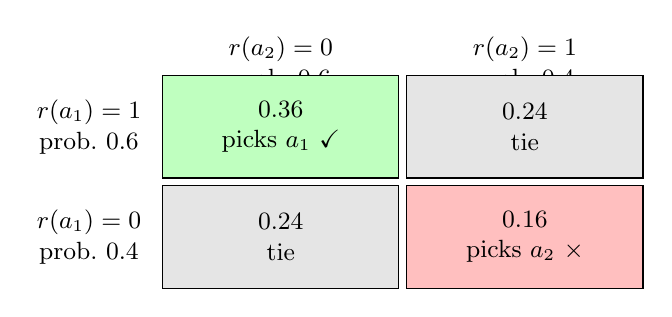
\begin{tikzpicture}[font=\small,every node/.style={align=center}]
  \foreach \i/\l in {0/{$r(a_2)=0$\\ prob.\ $0.6$},1/{$r(a_2)=1$\\ prob.\ $0.4$}}
     \node at (3.1*\i+1.55,2.7) {\l};
  \node[left] at (-0.1,1.9) {$r(a_1)=1$\\ prob.\ $0.6$};
  \node[left] at (-0.1,0.5) {$r(a_1)=0$\\ prob.\ $0.4$};
  \node[draw,fill=green!25,minimum width=3cm,minimum height=1.3cm] at (1.55,1.9) {$0.36$\\ picks $a_1$ \checkmark};
  \node[draw,fill=black!10,minimum width=3cm,minimum height=1.3cm] at (4.65,1.9) {$0.24$\\ tie};
  \node[draw,fill=black!10,minimum width=3cm,minimum height=1.3cm] at (1.55,0.5) {$0.24$\\ tie};
  \node[draw,fill=red!25,minimum width=3cm,minimum height=1.3cm] at (4.65,0.5) {$0.16$\\ picks $a_2$ $\times$};
\end{tikzpicture}
\caption{Outcomes of the first two pulls in the greedy example (probabilities multiply because the arms are independent).}
\end{figure}

\begin{intuition}
Greedy treats one noisy sample as the truth. If ties are broken uniformly, the probability of locking onto
the worse arm is $0.16+0.24=0.40$ (not just the $16\%$ highlighted on the slide), and once committed it loses
$0.2$ per round forever, so the expected regret is about $0.4\times0.2\,T=0.08\,T$: \emph{linear} in $T$.
Any sensible algorithm must keep sampling long enough to be confident.
\end{intuition}

\subsection{Explore \& Commit Algorithm \slides{8}}

\begin{algorithm}[Explore-then-commit, MAB]
Choose an exploration length $N$ per arm (the slide writes $N=T/K$ as a placeholder; it must satisfy $NK\ll T$, and
the optimised value is derived on slide~12).
\begin{enumerate}
  \item \textbf{Explore.} For $k=1,\dots,K$: pull arm $k$ exactly $N$ times and compute the empirical mean
        $\hat\mu_k=\frac1N\sum_{i=1}^N r_i$.
  \item \textbf{Commit.} For $t=NK,\dots,T-1$: pull $\hat I=\argmax_{i\in[K]}\hat\mu_i$.
\end{enumerate}
\end{algorithm}

\subsection{Hoeffding Inequality \slides{9--10}}

To say how wrong $\hat\mu$ can be, we need a confidence interval.

\begin{theorem}[Hoeffding inequality (Lecture~1, Thm.~5)]\label{thm:hoeffding}
Let $X_1,\dots,X_N\in[0,1]$ be i.i.d.\ with mean $\mu$. For every $\delta\in(0,1)$, with probability at least $1-\delta$,
\[
 \Bigl|\tfrac1N\textstyle\sum_{i=1}^N X_i-\mu\Bigr|\;\le\;\sqrt{\frac{\ln(2/\delta)}{2N}} \;=\;O\!\Bigl(\sqrt{\tfrac{\ln(1/\delta)}{N}}\Bigr).
\]
Applying it to all $K$ arms at once with a union bound (replace $\delta$ by $\delta/K$) gives, with probability at least $1-\delta$,
$|\hat\mu_i-\mu_i|\le\sqrt{\ln(2K/\delta)/(2N)}$ \emph{simultaneously} for every arm $i$.
\end{theorem}

\begin{figure}[ht]
\centering
\begin{tikzpicture}[font=\small]
  \begin{scope}
    \civ{0}{2}{1.55}{2}
    \node[left] at (-0.15,4) {$\hat\mu+\sqrt{\ln(1/\delta)/N}$};
    \node[left] at (-0.15,2) {$\hat\mu$};
    \node[left] at (-0.15,0) {$\hat\mu-\sqrt{\ln(1/\delta)/N}$};
    \node[right,green!50!black] at (0.15,1.55) {$\mu$ (unknown, inside the interval w.p.\ $1-\delta$)};
  \end{scope}
  \begin{scope}[xshift=8.2cm]
    \draw[->] (-0.3,-0.6) -- (-0.3,4.4) node[above] {reward};
    \civ{1}{2.1}{1.75}{0.9}  \civ{2.5}{2.7}{2.5}{0.9}  \civ{4}{1.5}{1.8}{0.9}
    \foreach \x/\a in {1/1,2.5/2,4/3} \node[below] at (\x,-0.1) {arm $\a$};
    \draw[dotted] (0.6,3.0) -- (4.4,3.0) (0.6,1.2) -- (4.4,1.2);
    \node[font=\scriptsize,align=center] at (2.5,4.3) {same width $\sqrt{\ln(K/\delta)/N}$ for all arms};
  \end{scope}
\end{tikzpicture}
\caption{Left (slide 9): the confidence interval around one empirical mean; the true mean (green) lies inside with
probability $1-\delta$. Right (slide 10): during commitment, all $K$ intervals hold simultaneously, so the width
contains $\ln(K/\delta)$. Black dots: $\hat\mu_i$ and interval ends.}
\end{figure}

\begin{intuition}
The interval shrinks like $1/\sqrt N$: to halve the uncertainty you need four times the data. With $\delta=0.01$
(``the bound holds with probability 99\%'') and $N=100$ samples, the half-width is
$\sqrt{\ln(200)/200}\approx0.163$; with $N=1000$ it is $\approx0.051$. For $K=10$ arms and $N=100$, the union bound
makes it $\sqrt{\ln(2000)/200}\approx0.195$: the price of ``all arms at once'' is only logarithmic in $K$.
\end{intuition}

\subsection{Regret Calculation \slides{11--12}}

Let $\hat I=\argmax_i\hat\mu_i$ (empirical best arm) and $I^\star=\argmax_i\mu_i$ (best arm).

\begin{theorem}[Regret of explore-then-commit, MAB]\label{thm:ec-mab}
Let $L=\ln(2K/\delta)$ (the slides write $\ln(K/\delta)$, absorbing constants into the $O(\cdot)$) and $1\le NK\le T$. With probability at least $1-\delta$,
\[
 \Reg_T=\Reg_{\mathrm{explore}}+\Reg_{\mathrm{exploit}}\;\le\; NK+2T\sqrt{\frac{L}{N}} .
\]
Choosing $N^\star=\bigl(T\sqrt{L}/K\bigr)^{2/3}$ gives
$\Reg_T\le 3\,T^{2/3}K^{1/3}L^{1/3}=O\bigl(T^{2/3}K^{1/3}\ln^{1/3}(K/\delta)\bigr)$.
\end{theorem}
\begin{proof}
Let $\varepsilon=\sqrt{L/(2N)}$. By Theorem~\ref{thm:hoeffding} all $|\hat\mu_i-\mu_i|\le\varepsilon$ on an event of probability $\ge1-\delta$. On it,
\[
 \mu_{I^\star}\le\hat\mu_{I^\star}+\varepsilon\le\hat\mu_{\hat I}+\varepsilon\le\mu_{\hat I}+2\varepsilon ,
\]
so every committed round costs at most $2\varepsilon$. Exploration lasts $NK$ rounds with per-round regret $\le1$, so
$\Reg_{\mathrm{explore}}\le NK$, and $\Reg_{\mathrm{exploit}}\le(T-NK)\,2\varepsilon\le 2T\sqrt{L/N}$.
For the second claim let $f(N)=NK+2T\sqrt L\,N^{-1/2}$. Then $f'(N)=K-T\sqrt L\,N^{-3/2}$ vanishes at $N^\star=(T\sqrt L/K)^{2/3}$
and $f$ is convex, so this is the minimiser. From $N^{\star3/2}=T\sqrt L/K$ we get $2T\sqrt L\,N^{\star-1/2}=2KN^\star$, hence
$f(N^\star)=3KN^\star=3K^{1/3}T^{2/3}L^{1/3}$ (ignoring rounding of $N^\star$).
\end{proof}

\begin{figure}[ht]
\centering
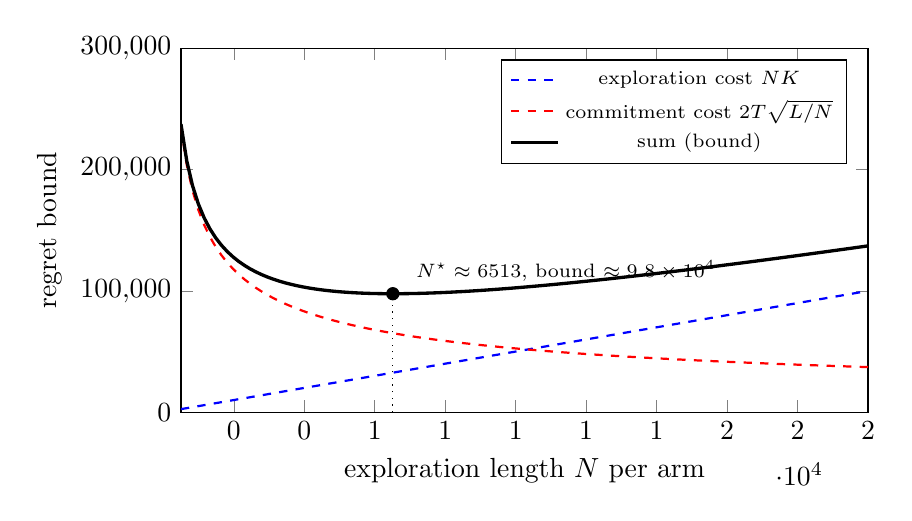
\begin{tikzpicture}
\begin{axis}[width=0.85\linewidth,height=6.2cm,xlabel={exploration length $N$ per arm},ylabel={regret bound},
  xmin=500,xmax=20000,ymin=0,ymax=300000,domain=500:20000,samples=120,no markers,
  legend style={font=\scriptsize,at={(0.97,0.97)},anchor=north east},scaled y ticks=false,
  yticklabel style={/pgf/number format/fixed,/pgf/number format/precision=0},
  xticklabel style={/pgf/number format/fixed,/pgf/number format/precision=0}]
 \addplot[blue,dashed,thick]{5*x};
 \addplot[red,dashed,thick]{2*1000000*sqrt(6.9078/x)};
 \addplot[black,very thick]{5*x+2*1000000*sqrt(6.9078/x)};
 \addlegendentry{exploration cost $NK$}
 \addlegendentry{commitment cost $2T\sqrt{L/N}$}
 \addlegendentry{sum (bound)}
 \addplot[only marks,mark=*,mark size=2.2pt,black,forget plot] coordinates {(6513,97700)};
 \draw[dotted] (axis cs:6513,0) -- (axis cs:6513,97700);
 \node[anchor=south west,font=\scriptsize] at (axis cs:6900,100000) {$N^\star\approx 6513$, bound $\approx 9.8\times10^4$};
\end{axis}
\end{tikzpicture}
\caption{The explore/exploit trade-off inside Theorem~\ref{thm:ec-mab} for $T=10^6$, $K=5$, $\delta=0.01$ ($L\approx6.91$):
more exploration costs linearly, but shrinks the commitment error like $1/\sqrt N$.}
\end{figure}

\begin{intuition}
Too little exploration makes you commit to the wrong arm; too much wastes rounds on bad arms. The optimum balances the
two curves (at $N^\star$ the commitment term is exactly twice the exploration term). Numerically, for $T=10^6$,
$K=5$, $\delta=0.01$: $N^\star\approx6{,}513$ pulls per arm, i.e.\ $\approx32{,}600$ exploration rounds (3.3\% of $T$), and
a regret bound of $\approx9.8\times10^4$, about $9.8\%$ of the maximum possible. Dividing by $T$, the \emph{average}
regret per round decays like $T^{-1/3}$, i.e.\ it ``approaches~0 as $T\to\infty$'' (slide~12), but slowly.
\end{intuition}

\subsection{Regret Decaying \slides{13}}

The $T^{2/3}$ rate of explore-then-commit is ``kind of slow''. The slide asks for something like $O(\sqrt T)$ and states that
$\sqrt T$ is the best possible: it is a \emph{lower bound}, no algorithm can do better in the worst case
(the standard minimax bound is $\Omega(\sqrt{KT})$; it is quoted, not proved, in the lecture). So we look for a new algorithm.

\begin{figure}[ht]
\centering
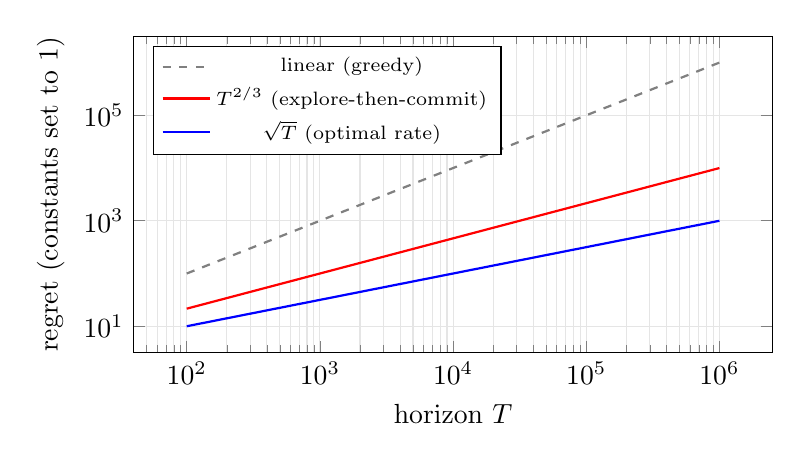
\begin{tikzpicture}
\begin{loglogaxis}[width=0.8\linewidth,height=5.6cm,xlabel={horizon $T$},ylabel={regret (constants set to 1)},
  domain=1e2:1e6,samples=40,no markers,legend style={font=\scriptsize,at={(0.03,0.97)},anchor=north west},grid=both,
  grid style={black!10}]
 \addplot[gray,dashed,thick]{x};
 \addplot[red,thick]{x^(2/3)};
 \addplot[blue,thick]{x^(1/2)};
 \addlegendentry{linear (greedy)}
 \addlegendentry{$T^{2/3}$ (explore-then-commit)}
 \addlegendentry{$\sqrt T$ (optimal rate)}
\end{loglogaxis}
\end{tikzpicture}
\caption{Growth rates compared (slide 13 describes them in words). On a log--log plot a rate $T^\alpha$ is a line of slope~$\alpha$.}
\end{figure}

\begin{intuition}
For $T=10^6$: $\sqrt T=10^3$ versus $T^{2/3}=10^4$. A tenfold gap, i.e.\ per-round regret $0.1\%$ versus $1\%$ (with all constants set to~1).
\end{intuition}

\subsection{Statistics to Maintain \& Confidence \slides{14}}

To compute confidence bounds \emph{while} learning we keep, for each arm $i$ at time $t$:
\[
 N_t(i)=\sum_{\tau=0}^{t-1}\ind\{I_\tau=i\},\qquad
 \hat\mu_t(i)=\frac{1}{N_t(i)}\sum_{\tau=0}^{t-1}\ind\{I_\tau=i\}\,r_\tau ,
\]
and, with probability $1-\delta$ (simultaneously for all arms and all times),
\[
 |\hat\mu_t(i)-\mu_i|\le\sqrt{\frac{\ln(KT/\delta)}{N_t(i)}} .
\]

\begin{intuition}
Unlike explore-then-commit, arms now have \emph{different} sample sizes, so each arm gets its \emph{own} interval width.
The $KT$ inside the logarithm is a union bound over every (arm, time) pair, because the algorithm will consult these bounds at every round.
\end{intuition}

\subsection{Optimism in the Face of Uncertainty \slides{15}}

Pick the arm with the highest \emph{upper} confidence bound (the top of its interval).

\begin{figure}[ht]
\centering
\begin{tikzpicture}[font=\small,y=3.4cm]
  \civ{1}{0.55}{0.5}{0.2}  \civ{3.2}{0.5}{0.6}{0.35}  \civ{5.4}{0.6}{0.58}{0.1}
  \foreach \x/\a in {1/1,3.2/2,5.4/3} \node[below=3pt] at (\x,0.15) {arm $\a$};
  \draw[red!70!black,thick,rounded corners=2pt] (2.7,0.78) rectangle (3.7,0.92);
  \draw[dotted,red!70!black] (0.6,0.85) -- (6.0,0.85);
  \node[red!70!black,right,font=\footnotesize] at (6.0,0.85) {highest UCB $\Rightarrow$ play arm 2};
  \node[font=\footnotesize,align=center] at (1,1.15) {tried often\\(medium)};
  \node[font=\footnotesize,align=center] at (3.2,1.35) {tried rarely\\(wide)};
  \node[font=\footnotesize,align=center] at (5.4,0.98) {tried a lot\\(narrow)};
  \draw[->] (-0.5,0.0) -- (-0.5,1.2) node[above] {reward};
\end{tikzpicture}
\caption{Optimism (slide 15). Arm~2 has a \emph{lower} empirical mean than arm~3, but its wide interval (few pulls) gives the highest upper bound, so UCB explores it.
Green dots: true means.}
\end{figure}

\subsection{UCB Algorithm \slides{16}}

\begin{algorithm}[UCB]\label{alg:ucb}
Pull each arm once (first $K$ rounds). For $t=K,\dots,T-1$:
\begin{enumerate}
  \item pick $\displaystyle I_t=\argmax_{i\in[K]}\Bigl(\hat\mu_t(i)+\sqrt{\tfrac{\ln(KT/\delta)}{N_t(i)}}\Bigr)$;
  \item observe the reward and update $N_t,\hat\mu_t$.
\end{enumerate}
The square-root \emph{reward bonus} is large for arms not tried many times, which drives exploration.
\end{algorithm}

\begin{intuition}
UCB acts as if each arm were as good as it \emph{could plausibly be}. Under-sampled arms get an inflated score and are tried;
if the optimism was unjustified, the empirical mean drops and $N_t(i)$ grows, so the bonus shrinks and the arm is abandoned.
Nothing is hard-coded about \emph{when} to stop exploring: the schedule emerges from the data. Exploration and exploitation are fused into one rule.
\end{intuition}

\subsection{UCB Algorithm: Regret \slides{17}}

\begin{theorem}[Regret of UCB (Lecture~1)]\label{thm:ucb}
Let $L'=\ln(2KT/\delta)$. With probability at least $1-\delta$, UCB satisfies
$\Reg_T\le K+4\sqrt{KT\,L'}=\widetilde O(\sqrt{KT})$.
\end{theorem}
\begin{proof}
On the event that all intervals hold, write $w_t=\sqrt{L'/N_t(I_t)}$. Then
\[
 \mu^\star\le \hat\mu_t(I^\star)+\sqrt{\tfrac{L'}{N_t(I^\star)}}\le \hat\mu_t(I_t)+w_t\le\mu_{I_t}+2w_t,
\]
so the per-round regret is $\mu^\star-\mu_{I_t}\le 2w_t$ (the first inequality is validity of the interval for $I^\star$, the second is the UCB rule, the third is validity for $I_t$). Summing over $t\ge K$,
\[
 \sum_{t=K}^{T-1}\frac1{\sqrt{N_t(I_t)}}=\sum_{i}\sum_{n=1}^{N_T(i)-1}\frac1{\sqrt n}\le\sum_i 2\sqrt{N_T(i)}\le 2\sqrt{K\textstyle\sum_iN_T(i)}\le2\sqrt{KT},
\]
by $\sum_{n\le m}n^{-1/2}\le2\sqrt m$ and Cauchy--Schwarz. The first $K$ rounds cost at most $K$. Hence $\Reg_T\le K+2\sqrt{L'}\cdot2\sqrt{KT}$.
\end{proof}

\begin{intuition}
Each arm contributes $\sum_{n\le N}1/\sqrt n\approx2\sqrt N$ to the regret sum, and the total number of pulls is capped at $T$; the worst case is spreading
pulls evenly, which yields $\sqrt{KT}$. For $K=5$, $T=10^6$ the \emph{rate} is $\approx\sqrt{5\cdot10^6}\approx2.2\times10^3$ (times $\sqrt{\ln}$ and a constant),
versus the $T^{2/3}$ rate of explore-then-commit which is of order $10^4$. (The slide cites an external note for details, \url{https://wensun.github.io/CS4789_data/UCB_note_new.pdf}.)
\end{intuition}
% =====================================================================
\section{From Multi-Armed to Contextual Bandits \slides{19--24}}

\subsection{From Multi-Armed to Contextual Bandits \slides{19--20}}

A multi-armed bandit is \emph{stateless}: an action leads to a reward. A \textbf{contextual bandit} adds a context (state)
that is observed before acting and that influences which action is best.

\begin{figure}[ht]
\centering
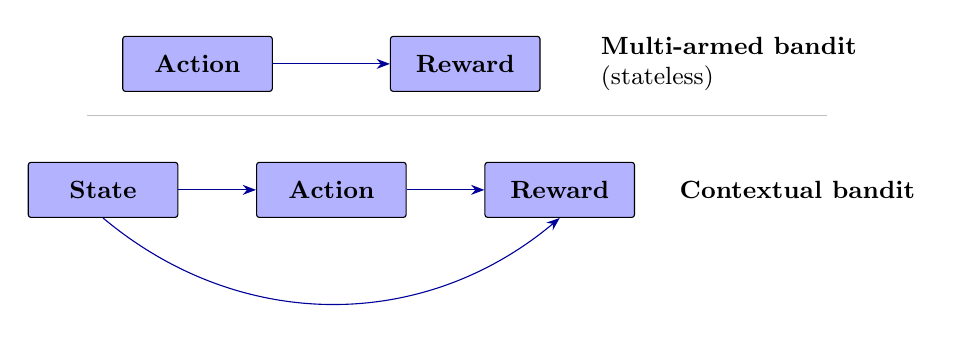
\begin{tikzpicture}[>=Stealth,font=\small,
  blk/.style={draw,fill=blue!30,rounded corners=1pt,minimum width=1.9cm,minimum height=0.7cm,font=\small\bfseries}]
  \node[blk] (a1) at (0,1.6) {Action};  \node[blk] (r1) at (3.4,1.6) {Reward};
  \draw[->,blue!60!black] (a1) -- (r1);
  \node[align=left,anchor=west] at (5.0,1.6) {\textbf{Multi-armed bandit}\\ (stateless)};
  \draw[black!25] (-1.4,0.95) -- (8,0.95);
  \node[blk] (s2) at (-1.2,0) {State};  \node[blk] (a2) at (1.7,0) {Action};  \node[blk] (r2) at (4.6,0) {Reward};
  \draw[->,blue!60!black] (s2) -- (a2);  \draw[->,blue!60!black] (a2) -- (r2);
  \draw[->,blue!60!black] (s2.south) to[bend right=40] (r2.south);
  \node[align=left,anchor=west] at (6.0,0) {\textbf{Contextual bandit}};
\end{tikzpicture}
\caption{Slides 19--20 redrawn. In a contextual bandit the reward depends on the \emph{state/context and the action}
(the curved arrow).}
\end{figure}

\subsection{Contextual Bandits: Interaction \slides{21--23}}

\begin{definition}[Contextual bandit]\label{def:cb}
A contextual bandit is a distribution $\rho$ over a context set $\calX$ together with a mean-reward function
$r:\calX\times\calA\to[0,1]$, where $|\calA|=K$. For $t=0,1,\dots,T-1$:
\begin{enumerate}
 \item a context $x_t\sim\rho$ is drawn i.i.d.\ and \emph{revealed};
 \item the learner picks $a_t\in\calA$, possibly at random, using $x_t$ and the history;
 \item a reward $r_t$ with $\E[r_t\mid x_t,a_t]=r(x_t,a_t)$ is revealed, and nothing is revealed about the other $K-1$ actions.
\end{enumerate}
\end{definition}

\begin{remark}
For simplicity the slides (slide~22) assume \emph{deterministic} rewards $r_t=r(x_t,a_t)$, ``as the context is the challenge here'';
the companion note stresses that every result below holds with noisy rewards too (the proof of Lemma~\ref{lem:ips}
conditions on the noise).
\end{remark}

\begin{figure}[ht]
\centering
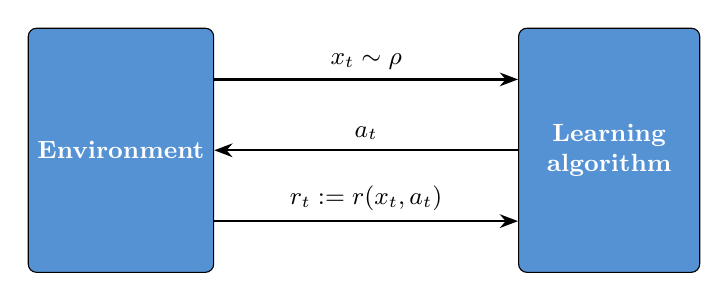
\begin{tikzpicture}[>=Stealth,font=\small,
  box/.style={draw,fill=cyan!55!blue!70,rounded corners=3pt,minimum width=2.3cm,minimum height=3.1cm,text=white,align=center,font=\small\bfseries}]
  \node[box] (env) at (0,0) {Environment};
  \node[box] (alg) at (6.2,0) {Learning\\algorithm};
  \draw[->,thick] ($(env.east)+(0,0.9)$) -- node[above] {$x_t\sim\rho$} ($(alg.west)+(0,0.9)$);
  \draw[->,thick] ($(alg.west)+(0,0)$) -- node[above] {$a_t$} ($(env.east)+(0,0)$);
  \draw[->,thick] ($(env.east)+(0,-0.9)$) -- node[above] {$r_t:=r(x_t,a_t)$} ($(alg.west)+(0,-0.9)$);
\end{tikzpicture}
\caption{The interaction protocol (slide 23). After the reward, a new round starts: contexts are \emph{not} influenced by past actions, they are sampled i.i.d.}
\end{figure}

\begin{intuition}
The i.i.d.\ context is what separates a contextual bandit from a full MDP: your action affects your \emph{reward} today but not the \emph{state}
you will see tomorrow, so there are no long-term consequences to plan around. It is a bandit with side information. The difficulty that remains is that
the best action depends on the context, and you only see the reward of the action you actually took.
\end{intuition}

\subsection{Contextual Bandits: Example \slides{24}}

A major application is \textbf{recommendation systems}: the \emph{context} is user information (age, height, weight, job, \dots), the \emph{arms} are items to recommend
(news, movies, \dots), and each arm has a click-through rate (0/1 reward) that we want to maximise. The question: how do we decide which item to propose next \emph{in a personalised way}?

\begin{example}\label{ex:reco}
Two equally frequent user types and two items, with click-through rates

\smallskip
\begin{center}
\begin{tabular}{lcc}\toprule
 & news & movies\\\midrule
 younger users & $0.10$ & $0.30$\\ older users & $0.35$ & $0.15$\\\bottomrule
\end{tabular}
\end{center}
A context-blind bandit sees an average CTR of $0.225$ for both items and earns $0.225$ per round at best, whereas the personalised rule
(movies for younger, news for older) earns $\tfrac12(0.30+0.35)=0.325$.
\end{example}

\begin{intuition}
Ignoring context averages away exactly the structure that matters. But learning one separate bandit per context is hopeless when contexts are
many or continuous (every user is unique). The remedy, developed next, is to learn a \emph{policy} from a restricted class $\Pi$ that generalises across contexts.
\end{intuition}

% =====================================================================
\section{Policy \slides{25}}

\begin{definition}[Policy]\label{def:policy}
A policy $\pi$ is a mapping from (all) states/contexts to actions that determines how the agent selects actions. It can be
\emph{deterministic}, $a=\pi(x)$, or \emph{stochastic}, $\pi(a\mid x)$ (equivalently $a\sim\pi(\cdot\mid x)$). Given a class $\Pi$ of policies, the
\emph{value} of $\pi$ is its expected reward, $V(\pi)=\E_{x\sim\rho}\bigl[r(x,\pi(x))\bigr]$.
\end{definition}

\begin{intuition}
A policy is a rulebook: ``if the user looks like this, show that''. For a finite context set $\calX$ with $K$ actions there are $K^{|\calX|}$ deterministic policies:
with $|\calX|=10$ and $K=3$ that is $3^{10}=59{,}049$, huge, but its \emph{logarithm} is only $10\ln3\approx10.99$. It is this logarithm, $\ln|\Pi|$, that will govern the regret.
\end{intuition}

% =====================================================================
\section{Contextual Bandits: Regret \slides{26}}

The optimal policy in the class is $\pi^\star=\argmax_{\pi\in\Pi}\E_{x\sim\rho}\,r(x,\pi(x))=\argmax_{\pi\in\Pi}V(\pi)$.
At every round $a_t=\pi_t(x_t)$ is selected and a reward received.

\begin{definition}[Contextual regret]\label{def:reg}
\[
 \mathrm{Reg}(T)\;=\;T\,V(\pi^\star)-\sum_{t=0}^{T-1}V(\pi_t)
 \;=\;T\,\E_{x\sim\rho}\bigl[r(x,\pi^\star(x))\bigr]-\sum_{t=0}^{T-1}\E_{x\sim\rho}\bigl[r(x,\pi_t(x))\bigr],
\]
where $\pi_t$ is the policy the learner is using at round $t$ (note: \emph{it changes at every iteration}).
\end{definition}

\begin{intuition}
The first term is the total expected reward if we always used the best policy; the second is what our sequence of learned policies earns.
If $\calX$ is a single context, $V(\pi)=r(a)$ and this is exactly the multi-armed regret of Section~1. In the recommendation example the
best policy earns $0.325$ per round, so a context-blind learner has regret at least $(0.325-0.225)T=0.1\,T$, linear in $T$.
\end{intuition}

% =====================================================================
\section{Explore \& Commit Algorithm \slides{27--31}}

\subsection{The algorithm \slides{27}}

\begin{algorithm}[Explore-then-commit for contextual bandits]\label{alg:ec}
Input: horizon $T$, policy class $\Pi$, exploration budget $N$.
\begin{enumerate}
 \item \textbf{Explore.} For $t=0,\dots,N-1$: observe $x_t\sim\rho$, draw $a_t\sim\Unif(\calA)$, observe $r_t=r(x_t,a_t)$, and build for $x_t$ an
       \emph{unbiased estimate} $\rh_t$ of the reward vector $\bigl(r(x_t,a)\bigr)_{a\in\calA}$.
 \item \textbf{Fit.} Compute the policy $\displaystyle\hat\pi\in\argmax_{\pi\in\Pi}\sum_{t=0}^{N-1}\rh_t[\pi(x_t)]$.
 \item \textbf{Commit.} For $t=N,\dots,T-1$: observe $x_t\sim\rho$ and play $a_t=\hat\pi(x_t)$.
\end{enumerate}
\end{algorithm}

The missing ingredient is the unbiased estimate $\rh_t$: we only observe the reward of \emph{one} action.

\subsection{Unbiased estimates: inverse propensity scoring \slides{27--29}}

An estimator $\hat\theta$ is \emph{unbiased} if $\E[\hat\theta]=\theta$, i.e.\ $\mathrm{bias}(\hat\theta)=\E[\hat\theta]-\theta=0$ (it is centred on the true value).
The goal here: $\E_{a_t\sim p}\bigl[\rh_t[a]\bigr]=r(x_t,a)$ for all $a$.

\begin{definition}[Inverse propensity scoring (IPS)]\label{def:ips}
Suppose that at round $t$ the action was drawn from a \emph{known} distribution $p_t$ with $p_t(a)>0$ for all $a$. The IPS reward vector is
\[
 \rh_t[a]=\frac{r_t\,\ind[a_t=a]}{p_t(a)},\qquad a\in\calA,
\]
i.e.\ the vector with a single non-zero entry $r_t/p_t(a_t)$ at the played action. Under uniform exploration, $p_t(a)=1/K$ and
$\rh_t[a]=\bigl\{K r_t$ if $a=a_t$, $0$ otherwise$\bigr\}$ (slide 29: ``$r_t/(1/|\calA|)$'').
\end{definition}

\begin{lemma}[IPS is unbiased]\label{lem:ips}
For every context $x_t$ and every action $a$, $\E_{a_t\sim p_t}\bigl[\rh_t[a]\mid x_t\bigr]=r(x_t,a)$. Consequently
$\E\bigl[\rh_t[\pi(x_t)]\bigr]=V(\pi)$ for every policy $\pi$.
\end{lemma}
\begin{proof}
Condition on $x_t$ and take the expectation over $a_t\sim p_t$ and the reward noise:
\[
 \E\!\left[\frac{r_t\,\ind[a_t=a]}{p_t(a)}\right]=\sum_{a'\in\calA}p_t(a')\,\frac{\E[r_t\mid x_t,a']\,\ind[a'=a]}{p_t(a)}
 =p_t(a)\,\frac{r(x_t,a)}{p_t(a)}=r(x_t,a).
\]
Averaging over $x_t\sim\rho$ gives $\E[\rh_t[\pi(x_t)]]=V(\pi)$.
\end{proof}

\begin{intuition}
The division by $p_t(a)$ ``removes the asymmetry due to sampling'' (slide 28): an action played half as often has its rewards counted twice as heavily,
exactly like survey weights that up-weight under-sampled groups. A concrete check with $K=2$, uniform exploration and $r(x,2)=0.8$: whenever arm~2 is played
(half the time) we record $\rh=(0,\,1.6)$, otherwise $(\cdot,\,0)$, so the average is $\tfrac12\cdot1.6+\tfrac12\cdot0=0.8$. The estimator is unbiased
but \emph{noisy}: a single observation is either $0$ or $Kr_t$, far from the true mean (made precise in Lemma~\ref{lem:range}, Appendix~\ref{app:supp}).
Importantly, $\rh_t$ is defined for \emph{all} actions even though only one is observed, which is what lets us evaluate policies that would have acted differently.
\end{intuition}

\subsection{Fitting a policy \slides{27}}

Step~2 of Algorithm~\ref{alg:ec} maximises the \emph{counterfactual value estimate}
$\hat V(\pi)=\frac1N\sum_{t<N}\rh_t[\pi(x_t)]$ over $\Pi$. By Lemma~\ref{lem:ips} each summand has mean $V(\pi)$, so $\hat V(\pi)$ estimates $V(\pi)$ for \emph{every} $\pi\in\Pi$ from the \emph{same} exploration data.

\begin{intuition}
Under uniform exploration, a round only ``counts'' for policy $\pi$ if $\pi(x_t)$ happens to equal the randomly played $a_t$ (probability $1/K$), and then it counts with weight $K r_t$.
In the toy problem below (two contexts, two arms) the four deterministic policies have values
$V(a_1,a_1)=0.525$, $V(a_1,a_2)=0.675$, $V(a_2,a_1)=0.425$, $V(a_2,a_2)=0.575$ (red~$\to$~first entry, blue~$\to$~second), so $\pi^\star=(a_1,a_2)$.
Because $\Pi$ here contains \emph{all} context-to-action maps, the maximisation splits into one independent argmax per context; for a restricted class (e.g.\ linear policies) it does not.
\end{intuition}

\subsection{Simulation \slides{30}}

Slide~30 shows an animation of the explore phase: a timeline of contexts (red/blue) and, per context, the running estimates of each arm's reward. Here is an original static version.

\begin{figure}[ht]
\centering
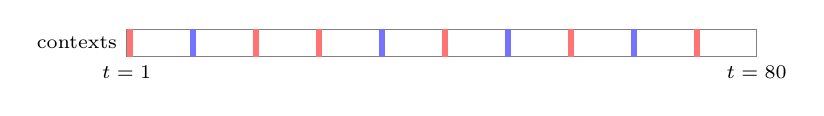
\begin{tikzpicture}
  \draw[black!50] (0,0) rectangle (8,0.35);
  \foreach \x/\c in {0/red!55,0.1/blue!55,0.2/red!55,0.3/red!55,0.4/blue!55,0.5/red!55,0.6/blue!55,0.7/red!55,0.8/blue!55,0.9/red!55} {
    \fill[\c] (8*\x,0) rectangle (8*\x+0.08,0.35);
  }
  \node[left,font=\scriptsize] at (0,0.175) {contexts};
  \node[below,font=\scriptsize] at (0,0) {$t=1$}; \node[below,font=\scriptsize] at (8,0) {$t=80$};
\end{tikzpicture}\\[4pt]
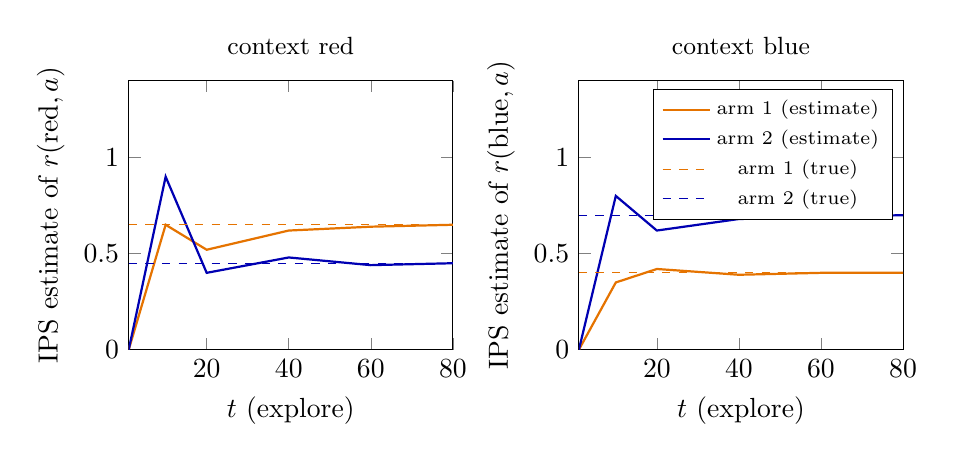
\begin{tikzpicture}
\begin{groupplot}[group style={group size=2 by 1,horizontal sep=1.6cm},width=0.47\linewidth,height=5cm,
  xmin=1,xmax=80,ymin=0,ymax=1.4,xlabel={$t$ (explore)},no markers,title style={font=\small}]
 \nextgroupplot[title={context red},ylabel={IPS estimate of $r(\text{red},a)$}]
  \addplot[orange!90!black,thick] coordinates {(1,0.00) (10,0.65) (20,0.52) (40,0.62) (60,0.64) (80,0.65)};
  \addplot[blue!70!black,thick] coordinates {(1,0.00) (10,0.90) (20,0.40) (40,0.48) (60,0.44) (80,0.45)};
  \addplot[orange!90!black,dashed] coordinates {(1,0.65) (80,0.65)};
  \addplot[blue!70!black,dashed] coordinates {(1,0.45) (80,0.45)};
 \nextgroupplot[title={context blue},ylabel={IPS estimate of $r(\text{blue},a)$},legend style={font=\scriptsize,at={(0.97,0.97)},anchor=north east}]
  \addplot[orange!90!black,thick] coordinates {(1,0.00) (10,0.35) (20,0.42) (40,0.39) (60,0.40) (80,0.40)};
  \addplot[blue!70!black,thick] coordinates {(1,0.00) (10,0.80) (20,0.62) (40,0.68) (60,0.69) (80,0.70)};
  \addplot[orange!90!black,dashed] coordinates {(1,0.40) (80,0.40)};
  \addplot[blue!70!black,dashed] coordinates {(1,0.70) (80,0.70)};
  \addlegendentry{arm 1 (estimate)}
 \addlegendentry{arm 2 (estimate)}
 \addlegendentry{arm 1 (true)}
 \addlegendentry{arm 2 (true)}
\end{groupplot}
\end{tikzpicture}
\caption{Toy simulation of the explore phase (seeded; $N=80$, uniform exploration, two equally likely contexts, deterministic rewards
$r(\text{red},\cdot)=(0.65,0.45)$, $r(\text{blue},\cdot)=(0.40,0.70)$). Solid: per-context IPS averages; dashed: true values. They are noisy at first but
settle on the correct ordering, so $\hat\pi=\pi^\star$ in this run (about $81\%$ of 2000 seeds at $N=80$).}
\end{figure}

\subsection{Explore \& Commit Algorithm: Regret \slides{31}}

The slide states that the regret ``also depends on the size of the class of policies''. Here is the precise statement.

\begin{theorem}[Regret of contextual explore-then-commit]\label{thm:cec}
Let $\Pi$ be finite and run Algorithm~\ref{alg:ec} with $1\le N\le T$. With probability at least $1-\delta$,
\[
 \mathrm{Reg}(T)\;\le\;N+TK\sqrt{\frac{2\ln(2|\Pi|/\delta)}{N}},
\]
and choosing $N$ to minimise the right-hand side gives
\[
 \mathrm{Reg}(T)\;\le\;3\cdot2^{-1/3}\,T^{2/3}K^{2/3}\ln^{1/3}\!\Bigl(\frac{2|\Pi|}{\delta}\Bigr).
\]
\end{theorem}
\begin{proof}
Write $\hat V(\pi)=\frac1N\sum_{t<N}\rh_t[\pi(x_t)]$. By Lemma~\ref{lem:ips} the summands are i.i.d.\ with mean $V(\pi)$ and by Lemma~\ref{lem:range} (Appendix~\ref{app:supp})
they lie in $[0,K]$. Hoeffding's inequality (Theorem~\ref{thm:hoeffding}, rescaled by $K$) gives, for one fixed $\pi$ and any $\delta'\in(0,1)$,
\[
 \Prob\Bigl(|\hat V(\pi)-V(\pi)|>K\sqrt{\ln(2/\delta')/(2N)}\Bigr)\le\delta'.
\]
Take $\delta'=\delta/|\Pi|$ and a union bound over the $|\Pi|$ policies: with probability at least $1-\delta$, every $\pi\in\Pi$ satisfies
$|\hat V(\pi)-V(\pi)|\le\varepsilon$ with $\varepsilon=K\sqrt{\ln(2|\Pi|/\delta)/(2N)}$.
On that event, the same three-step chain as in Theorem~\ref{thm:ec-mab} applies to $\hat\pi$, which maximises $\hat V$:
\[
 V(\pi^\star)\le\hat V(\pi^\star)+\varepsilon\le\hat V(\hat\pi)+\varepsilon\le V(\hat\pi)+2\varepsilon .
\]
Exploration contributes at most $N$ (each round's regret is at most $1$); commitment contributes at most $(T-N)\cdot2\varepsilon\le2T\varepsilon$. Adding them gives the first display.

For the second, set $c=\sqrt{2\ln(2|\Pi|/\delta)}$, so the bound reads $f(N)=N+TKc\,N^{-1/2}$. As in the MAB case, $f$ is convex and
$f'(N)=1-\tfrac12TKc\,N^{-3/2}$ vanishes at $N^\star=(TKc/2)^{2/3}$. Writing $u=(TKc/2)^{1/3}$ gives $f(N^\star)=u^2+2u^2=3(TKc/2)^{2/3}$, and substituting
$c^{2/3}=2^{1/3}\ln^{1/3}(2|\Pi|/\delta)$ gives the claim.
\end{proof}

\begin{intuition}
It is the same trade-off as in the MAB: exploring costs $N$ in regret; each extra sample sharpens \emph{all} policy estimates simultaneously, and the union bound over policies only
costs a $\ln|\Pi|$ factor inside the square root. Numerically, for $|\Pi|=10^6$, $K=3$, $\delta=0.05$, $T=10^6$: $\ln(2|\Pi|/\delta)\approx17.5$,
the optimal exploration length is $N^\star\approx4.3\times10^4$ rounds ($4.3\%$ of $T$) and the bound is $\approx1.29\times10^5$ ($12.9\%$ of $T$).
Making the class a million times richer, from $|\Pi|=10^6$ to $10^{12}$, multiplies the bound only by $(3.15/2.60)\approx1.21$ (the factor $\ln^{1/3}(2|\Pi|/\delta)$ goes $2.02\to2.60\to3.15$ for $|\Pi|=10^2,10^6,10^{12}$).
The price of context is thus \emph{logarithmic in the number of policies} but, because uniform exploration wastes a factor $K$ per observation, it grows with $K$.
\end{intuition}

\begin{remark}[On the exponent of $K$]
Slide~31 prints the bound as $O\bigl(T^{2/3}K^{1/3}\ln^{1/3}(|\Pi|)\bigr)$, while the proof above (which only uses the \emph{range} $[0,K]$ of the IPS terms) yields $K^{2/3}$.
The $K^{1/3}$ form is the known sharper rate: using the \emph{variance} bound of Lemma~\ref{lem:range} with Bernstein's inequality instead of Hoeffding's gives
deviations of order $\sqrt{K\ln(|\Pi|/\delta)/N}$ and hence $T^{2/3}K^{1/3}\ln^{1/3}(|\Pi|/\delta)$ plus a lower-order term. This refinement is a standard fact but is
\emph{not} proved in the companion note, so the theorem is stated with the exponent that is actually proved.
\end{remark}
% =====================================================================
\section{\texorpdfstring{$\epsilon$}{epsilon}-Greedy \slides{32--35}}

Instead of fixing a threshold for exploring and then committing, we can \emph{interleave} exploration and exploitation.

\begin{algorithm}[$\epsilon$-greedy for contextual bandits]\label{alg:eg}
For $t=0,1,\dots,T-1$:
\begin{enumerate}
 \item observe $x_t\sim\rho$;
 \item draw $a_t\sim p_t=(1-\epsilon_t)\,\delta\bigl(\pi^t(x_t)\bigr)+\epsilon_t\,\Unif(\calA)$;
 \item observe $r_t$ and form the IPS vector $\rh_t$ using the propensity $p_t(a_t)$ \emph{actually used};
 \item update the policy: $\pi^{t+1}\in\argmax_{\pi\in\Pi}\sum_{i\le t}\rh_i[\pi(x_i)]$.
\end{enumerate}
Gradually \textbf{decay} $\epsilon_t$ towards zero (slide 34, ``Step 3'').
\end{algorithm}

Here $\delta(\pi^t(x_t))$ is the Dirac delta placing all the mass on the action $\pi^t(x_t)$, so explicitly
$p_t(a)=(1-\epsilon_t)\ind[a=\pi^t(x_t)]+\epsilon_t/K$. The two extremes are $\epsilon=0$ (pure exploitation) and $\epsilon=1$ (uniform exploration).
Since $p_t(a)\ge\epsilon_t/K>0$, IPS is well defined, and Lemma~\ref{lem:ips} applies at every round (it only needs $p_t$ to be known, and $p_t$ may change with $t$).

\begin{figure}[ht]
\centering
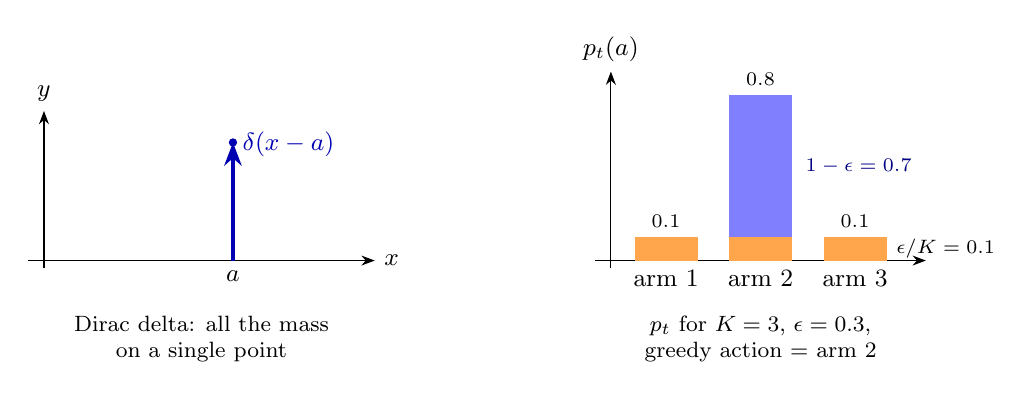
\begin{tikzpicture}[>=Stealth,font=\small]
 \begin{scope}
  \draw[->] (-0.2,0) -- (4.2,0) node[right] {$x$}; \draw[->] (0,-0.1) -- (0,1.9) node[above] {$y$};
  \draw[->,very thick,blue!70!black] (2.4,0) -- (2.4,1.5); \fill[blue!70!black] (2.4,1.5) circle (1.5pt);
  \node[blue!70!black,above right] at (2.4,1.2) {$\delta(x-a)$}; \node[below] at (2.4,0) {$a$};
  \node[align=center,font=\footnotesize] at (2,-1.0) {Dirac delta: all the mass\\on a single point};
 \end{scope}
 \begin{scope}[xshift=7.2cm]
  \draw[->] (-0.2,0) -- (4.0,0); \draw[->] (0,-0.1) -- (0,2.4) node[above] {$p_t(a)$};
  \foreach \x/\n in {0.7/1,1.9/2,3.1/3}{\node[below] at (\x,0) {arm \n};}
  \foreach \x in {0.7,1.9,3.1}{\fill[orange!70] (\x-0.4,0) rectangle (\x+0.4,0.3);}
  \fill[blue!50] (1.9-0.4,0.3) rectangle (1.9+0.4,2.1);
  \node[right,font=\scriptsize] at (3.5,0.15) {$\epsilon/K=0.1$};
  \node[right,font=\scriptsize,blue!50!black] at (2.35,1.2) {$1-\epsilon=0.7$};
  \node[above,font=\scriptsize] at (1.9,2.1) {$0.8$};
  \node[above,font=\scriptsize] at (0.7,0.3) {$0.1$}; \node[above,font=\scriptsize] at (3.1,0.3) {$0.1$};
  \node[align=center,font=\footnotesize] at (1.9,-1.0) {$p_t$ for $K=3$, $\epsilon=0.3$,\\greedy action $=$ arm 2};
 \end{scope}
\end{tikzpicture}
\caption{Left (slide 33): the Dirac delta used in $p_t$. Right: the resulting mixture: every arm gets a floor $\epsilon/K$ of exploration probability and the greedy arm additionally gets $1-\epsilon$.}
\end{figure}

\begin{intuition}
$\epsilon_t$ is a dial between ``trust what I have learned'' and ``roll a die''. The floor $\epsilon_t/K$ is what guarantees every action keeps being sampled so
that IPS stays valid. The dial must be turned down \emph{gradually}: from $r_t\le1$ and $p_t(a)\ge\epsilon_t/K$ we get $0\le\rh_t[a]\le K/\epsilon_t$, so if $\epsilon_t$
collapses, the estimates of rarely played actions become extremely noisy (e.g.\ $\epsilon_t=0.01$, $K=3$ allows values up to $300$). Note that, unlike
explore-then-commit, learning never stops, so the policy keeps adapting. (Neither the slides nor the companion note state a regret bound for $\epsilon$-greedy;
slide 35 only shows a simulation.)
\end{intuition}

\begin{figure}[H]
	\centering
	\includegraphics[width=1.0\linewidth]{1790925011807.png}
	\caption{Toy simulation of $\epsilon$-greedy (seeded, $T=90$): early on most rounds are exploratory (open red circles); as $\epsilon_t$ decays the learner mostly exploits its current policy, which here becomes
$\pi=(\text{red}\to\text{arm 1},\ \text{blue}\to\text{arm 2})=\pi^\star$ (27 of the 90 rounds were exploratory). This ends optimal in about $71\%$ of 1000 seeds at $t=90$, so individual runs vary; same colours and dashed true values as the earlier figure.}\label{fig:1790925011807}
\end{figure}




\section{Real World Example \slides{36}}

Slide 36 points to a production use of contextual-bandit algorithms: Microsoft's \emph{Azure Personalizer}
(\url{https://azure.microsoft.com/en-us/products/cognitive-services/personalizer/}), which the slide notes is \emph{going out of service in October 2026}
(the slide shows a screenshot of the product page, not reproduced here).

\begin{intuition}
Personalising content maps one-to-one onto the model of this lecture: the context is the user/page features, the actions are the candidate items, and the reward is a click or
other feedback. Each shown item produces feedback for \emph{that} item only, which is why IPS-style estimates and exploration are needed in practice. Whether a particular product is still available is a
separate matter from the algorithms, which remain standard.
\end{intuition}

% =====================================================================
\section{Bayes Theorem Recall \slides{37}}

\begin{theorem}[Bayes' theorem]\label{thm:bayes}
For a hypothesis $H$ and data $D$ with $p(D)>0$,
\[
 p(H\mid D)=\frac{p(H)\,p(D\mid H)}{p(D)} .
\]
\end{theorem}

\begin{figure}[ht]
\centering
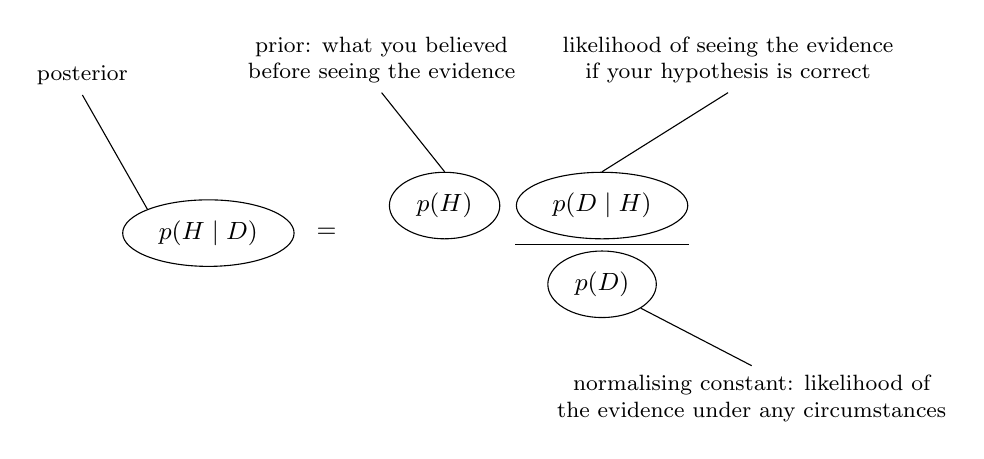
\begin{tikzpicture}[font=\small,>=Stealth]
  \node[draw,ellipse,inner sep=4pt] (post) at (0,0) {$p(H\mid D)$};
  \node at (1.5,0) {$=$};
  \node[draw,ellipse,inner sep=4pt] (prior) at (3.0,0.35) {$p(H)$};
  \node[draw,ellipse,inner sep=4pt] (lik) at (5.0,0.35) {$p(D\mid H)$};
  \draw (3.9,-0.15) -- (6.1,-0.15);
  \node[draw,ellipse,inner sep=4pt] (ev) at (5.0,-0.65) {$p(D)$};
  \node[align=center,font=\footnotesize] (t1) at (-1.6,2.0) {posterior};
  \node[align=center,font=\footnotesize] (t2) at (2.2,2.2) {prior: what you believed\\before seeing the evidence};
  \node[align=center,font=\footnotesize] (t3) at (6.6,2.2) {likelihood of seeing the evidence\\if your hypothesis is correct};
  \node[align=center,font=\footnotesize] (t4) at (6.9,-2.1) {normalising constant: likelihood of\\the evidence under any circumstances};
  \draw (t1.south) -- (post.north west);  \draw (t2.south) -- (prior.north);
  \draw (t3.south) -- (lik.north);        \draw (t4.north) -- (ev.south east);
\end{tikzpicture}
\caption{The annotated Bayes formula of slide 37.}
\end{figure}

\begin{intuition}
Posterior $\propto$ prior $\times$ likelihood; $p(D)$ only renormalises. Example: an ad is either \emph{good} (CTR $0.6$) or \emph{bad} (CTR $0.4$), prior $50/50$. After observing one click,
$p(\text{good}\mid\text{click})=\frac{0.5\cdot0.6}{0.5\cdot0.6+0.5\cdot0.4}=0.6$; after two clicks the odds multiply by $0.6/0.4$ again, giving odds $2.25$, i.e.\ $p\approx0.69$.
Each observation nudges belief towards the hypotheses that explain it best. This is the engine of Bayesian bandits.
\end{intuition}

% =====================================================================
\section{Bayesian Bandits \slides{38}}

So far we made \emph{no assumption} about the reward distributions $\nu_i$; we only derived bounds that hold for any bounded rewards. In \textbf{Bayesian bandits}:
\begin{itemize}
 \item we exploit \emph{prior} knowledge of the rewards;
 \item we update a \emph{posterior} distribution of rewards from the history;
 \item we use the posterior to guide exploration, via \textbf{upper confidence bounds} (Bayesian UCB) or \textbf{probability matching} (Thompson sampling).
\end{itemize}

\begin{intuition}
A frequentist guarantee protects you against \emph{any} reward distribution but is therefore conservative; a Bayesian method gets a head start when the prior is sensible (e.g.\ CTRs are mostly small) and the posterior directly
tells you ``how sure am I about each arm''. The price is that the guarantee is only as good as the modelling assumptions.
\end{intuition}

% =====================================================================
\section{Gaussian Bayesian Bandits Example \slides{39--40}}

\subsection{Setting \slides{39}}

Assume each reward distribution is Gaussian, $\nu_i=\Norm(\mu(i),\sigma^2(i))$. After some pulls the learner holds, for each arm, a belief (a Gaussian) about that arm's quality: the centre is the best guess
$\mu(i)$ and the width reflects remaining uncertainty.

\begin{figure}[ht]
\centering
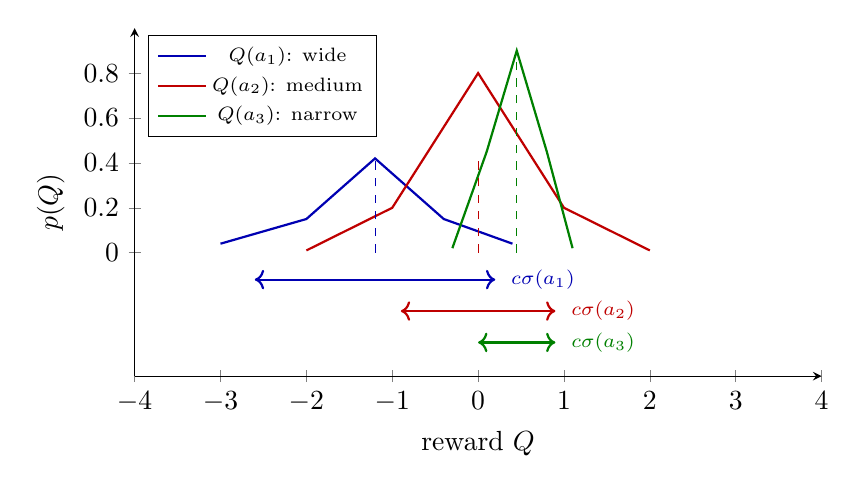
\begin{tikzpicture}
\begin{axis}[width=0.85\linewidth,height=6cm,xmin=-4,xmax=4,ymin=-0.55,ymax=1.0,xlabel={reward $Q$},ylabel={$p(Q)$},
  ytick={0,0.2,0.4,0.6,0.8},no markers,legend style={font=\scriptsize,at={(0.02,0.98)},anchor=north west},axis lines=left,clip=false]
 \addplot[blue!70!black,thick] coordinates {(-3,0.04) (-2,0.15) (-1.2,0.42) (-0.4,0.15) (0.4,0.04)};
 \addplot[red!75!black,thick] coordinates {(-2,0.01) (-1,0.20) (0,0.80) (1,0.20) (2,0.01)};
 \addplot[green!50!black,thick] coordinates {(-0.3,0.02) (0.1,0.45) (0.45,0.90) (0.8,0.45) (1.1,0.02)};
 \addlegendentry{$Q(a_1)$: wide}
 \addlegendentry{$Q(a_2)$: medium}
 \addlegendentry{$Q(a_3)$: narrow}
 \draw[dashed,blue!70!black] (axis cs:-1.2,0) -- (axis cs:-1.2,0.42);
 \draw[dashed,red!75!black] (axis cs:0,0) -- (axis cs:0,0.42);
 \draw[dashed,green!50!black] (axis cs:0.45,0) -- (axis cs:0.45,0.9);
 \draw[<->,blue!70!black,thick] (axis cs:-2.6,-0.12) -- (axis cs:0.2,-0.12) node[right,font=\scriptsize,xshift=2pt] {$c\sigma(a_1)$};
 \draw[<->,red!75!black,thick]  (axis cs:-0.9,-0.26) -- (axis cs:0.9,-0.26) node[right,font=\scriptsize,xshift=2pt] {$c\sigma(a_2)$};
 \draw[<->,green!50!black,thick](axis cs:0.0,-0.40) -- (axis cs:0.9,-0.40) node[right,font=\scriptsize,xshift=2pt] {$c\sigma(a_3)$};
\end{axis}
\end{tikzpicture}
\caption{Beliefs over the quality of three arms (slide 39 redrawn; dashed lines mark the means $\mu(a_i)$; the double arrows are confidence widths $\pm c\sigma$ around each mean). Arm~1 is very uncertain, arm~3 is well known.}
\end{figure}

\subsection{Posterior update \slides{40}}

The prior is often $\Norm(0,1)$. The posterior after history $h_t$ is proportional to the prior times the product of the likelihoods of all the rewards observed when this arm was selected (slide 40: ``product over all time-steps $t$ that select action $i$''). For a Gaussian prior and Gaussian noise this has a closed form.

\begin{proposition}[Gaussian conjugacy]\label{prop:gauss}
Let the unknown mean of an arm have prior $\mu\sim\Norm(m_0,s_0^2)$, and let $r_1,\dots,r_n$ be i.i.d.\ $\Norm(\mu,\sigma^2)$ with $\sigma^2$ known. Then the posterior is $\Norm(m_n,s_n^2)$ with
\[
 \frac1{s_n^2}=\frac1{s_0^2}+\frac n{\sigma^2},\qquad m_n=s_n^2\Bigl(\frac{m_0}{s_0^2}+\frac1{\sigma^2}\sum_{i=1}^nr_i\Bigr).
\]
\end{proposition}
\begin{proof}
By Bayes' rule (Theorem~\ref{thm:bayes}) the posterior density is proportional to prior times likelihood,
\[
 p(\mu\mid r_{1:n})\propto\exp\Bigl(-\frac{(\mu-m_0)^2}{2s_0^2}\Bigr)\prod_{i=1}^n\exp\Bigl(-\frac{(r_i-\mu)^2}{2\sigma^2}\Bigr).
\]
The exponent is a quadratic in $\mu$; collecting terms,
\[
 -\frac12\Bigl[\mu^2\Bigl(\frac1{s_0^2}+\frac n{\sigma^2}\Bigr)-2\mu\Bigl(\frac{m_0}{s_0^2}+\frac{\sum_ir_i}{\sigma^2}\Bigr)\Bigr]+\text{const},
\]
which is $-\frac1{2s_n^2}(\mu-m_n)^2+\text{const}$ for exactly the $s_n^2$ and $m_n$ of the statement. A density proportional to a Gaussian kernel is that Gaussian.
\end{proof}

\begin{corollary}[One-step update]\label{cor:gauss-step}
If arm $i$ has the posterior $\Norm(\mu_{t-1}(i),\sigma_{t-1}^2(i))$ and is pulled, yielding $r_t$, its new posterior is $\Norm(\mu_t(i),\sigma_t^2(i))$ with
\[
 \frac1{\sigma_t^2(i)}=\frac1{\sigma_{t-1}^2(i)}+\frac1{\sigma^2},\qquad
 \mu_t(i)=\sigma_t^2(i)\Bigl(\frac{\mu_{t-1}(i)}{\sigma_{t-1}^2(i)}+\frac{r_t}{\sigma^2}\Bigr);
\]
the posteriors of the other arms are unchanged.
\end{corollary}
\begin{proof}
Posterior updating can be done one observation at a time: the old posterior plays the role of the prior and Proposition~\ref{prop:gauss} is applied with $n=1$. Arms not pulled provide no data about their own mean, so their posteriors stay the same.
\end{proof}

This is the compact update shown on slide 40, $p(\mu_t(i),\sigma_t^2(i)\mid r_t)\propto p(\mu,\sigma^2)\,\Norm(r_t\mid\cdot)$: the slide writes the Gaussian likelihood of the new reward with the current posterior parameters as shorthand; the closed form above is what is actually computed.

\begin{figure}[ht]
\centering
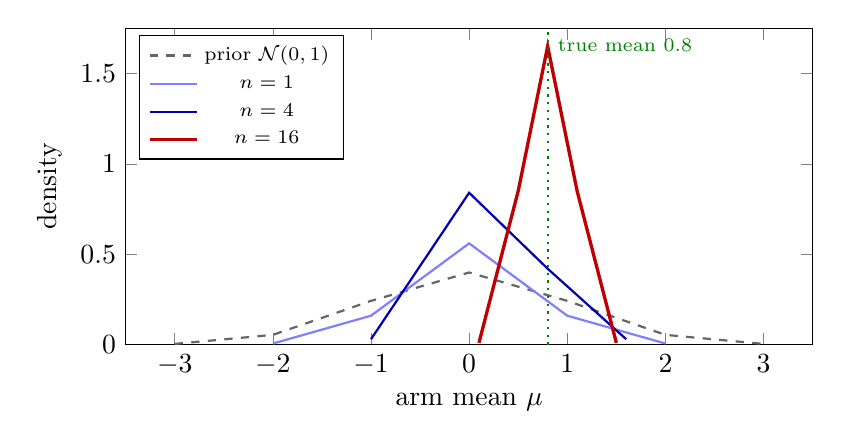
\begin{tikzpicture}
\begin{axis}[width=0.85\linewidth,height=5.6cm,xmin=-3.5,xmax=3.5,ymin=0,ymax=1.75,xlabel={arm mean $\mu$},ylabel={density},
 no markers,legend style={font=\scriptsize,at={(0.02,0.98)},anchor=north west}]
 \addplot[black!60,thick,dashed] coordinates {(-3,0.004) (-2,0.054) (-1,0.242) (0,0.399) (1,0.242) (2,0.054) (3,0.004)};
 \addplot[blue!50,thick] coordinates {(-2,0.006) (-1,0.16) (0,0.56) (1,0.16) (2,0.006)};
 \addplot[blue!70!black,thick] coordinates {(-1,0.03) (0,0.84) (0.8,0.42) (1.6,0.03)};
 \addplot[red!75!black,very thick] coordinates {(0.1,0.01) (0.5,0.85) (0.8,1.65) (1.1,0.85) (1.5,0.01)};
 \draw[dotted,thick,green!50!black] (axis cs:0.8,0) -- (axis cs:0.8,1.75) node[below right,font=\scriptsize] {true mean $0.8$};
 \addlegendentry{prior $\Norm(0,1)$}
 \addlegendentry{$n=1$}
 \addlegendentry{$n=4$}
 \addlegendentry{$n=16$}
\end{axis}
\end{tikzpicture}
\caption{Toy simulation of Proposition~\ref{prop:gauss} ($\sigma=1$, true mean $0.8$, seeded data): the posterior narrows like $1/\sqrt n$ (standard deviations $1,\ 0.71,\ 0.45,\ 0.24$ for $n=0,1,4,16$) and its centre drifts from the prior mean $0$ towards the truth
(posterior means $0.00$, $0.25$, $0.66$ for $n=1,4,16$ in this run).}
\end{figure}

\begin{intuition}
Precisions (inverse variances) \emph{add}: prior precision $1/s_0^2$ plus $1/\sigma^2$ per observation, and the posterior mean is a precision-weighted average of the prior mean and the data.
Worked example: prior $\Norm(0,1)$, $\sigma^2=1$, and $n=4$ observations summing to $3$. Then $s_4^2=1/(1+4)=0.2$ and $m_4=0.2\cdot(0+3)=0.6$: the sample mean $0.75$ is pulled slightly toward the prior mean~$0$ (like having one extra ``virtual'' observation equal to $0$).
The more data an arm has, the less the prior matters, and a rarely tried arm keeps a wide posterior, which is exactly what the exploration rules below exploit.
\end{intuition}

% =====================================================================
\section{Gaussian Bayesian Bandits: UCB \slides{41--43}}

Since we are modelling a distribution, we already have a measure of confidence. What is confidence for a Gaussian? Its \emph{standard deviation}. The slide proposes a UCB rule built from it:

\begin{algorithm}[Bayesian UCB (Gaussian)]\label{alg:bucb}
At round $t$ play
\[
 a_t=\argmax_{i\in[K]}\ \Bigl(\mu_t(i)+\frac{c\,\sigma_t(i)}{\sqrt{N_t(i)}}\Bigr),
\]
where $\mu_t(i)$ is the posterior mean, $N_t(i)$ the number of pulls of arm $i$, $\sigma_t(i)$ the Gaussian's standard deviation parameter and $c>0$ a constant that sets how optimistic we are.
\end{algorithm}

The slide's wording ``select the action with highest standard deviation'' is shorthand: the score is the mean plus $c$ times the uncertainty of the mean, $\sigma_t(i)/\sqrt{N_t(i)}$, which is the standard error of the arm's mean
(with a weak prior it coincides with the posterior standard deviation from Proposition~\ref{prop:gauss}).

\begin{figure}[ht]
\centering
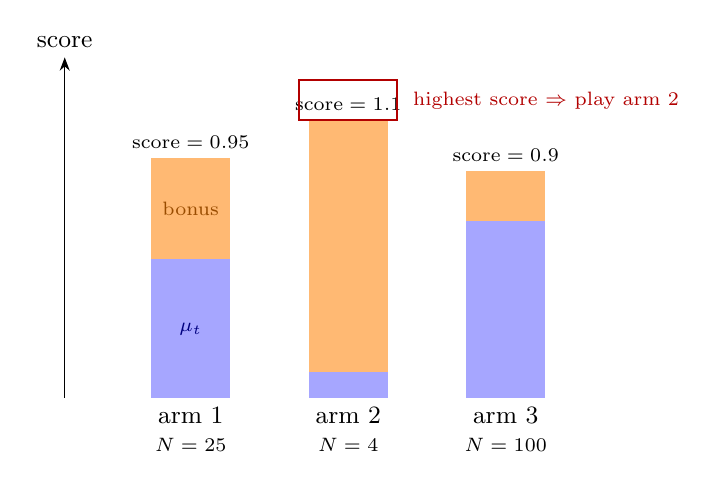
\begin{tikzpicture}[font=\small,>=Stealth,y=3.2cm]
  \draw[->] (-0.6,0) -- (-0.6,1.35) node[above] {score};
  \foreach \x/\mmu/\bon/\nn/\lab in {1/0.55/0.40/25/{$N=25$},3/0.10/1.00/4/{$N=4$},5/0.70/0.20/100/{$N=100$}}{
    \fill[blue!35] (\x-0.5,0) rectangle (\x+0.5,\mmu);
    \fill[orange!55] (\x-0.5,\mmu) rectangle (\x+0.5,\mmu+\bon);
    \node[below] at (\x,0) {arm \the\numexpr(\x+1)/2\relax};
    \node[below=11pt,font=\scriptsize] at (\x,0) {\lab};
    \pgfmathparse{\mmu+\bon}\let\score\pgfmathresult
    \node[above,font=\scriptsize] at (\x,\mmu+\bon) {$\mathrm{score}=\pgfmathprintnumber[fixed,precision=2]{\score}$};
  }
  \draw[red!70!black,thick] (3-0.62,1.10) rectangle (3+0.62,1.26);
  \node[blue!50!black,font=\scriptsize] at (1,0.27) {$\mu_t$};  \node[orange!60!black,font=\scriptsize] at (1,0.75) {bonus};
  \node[red!70!black,font=\scriptsize,right] at (3.7,1.18) {highest score $\Rightarrow$ play arm 2};
\end{tikzpicture}
\caption{Snapshot of Algorithm~\ref{alg:bucb} with $c=2$, $\sigma=1$ (illustrative numbers). Blue: posterior mean; orange: bonus $c\sigma/\sqrt{N}$. Arm~2 has the \emph{lowest} mean but is almost unexplored, so its bonus ($1.0$) lifts it to the top.}
\end{figure}

\begin{intuition}
Compare with Algorithm~\ref{alg:ucb}: the distribution-free width $\sqrt{\ln(KT/\delta)/N}$ is replaced by $c\sigma/\sqrt N$, with $c$ playing the role of $\sqrt{\ln(KT/\delta)}$. Under a Gaussian belief, $c=2$ means that the true mean lies below the score with probability
$\Phi(2)\approx97.7\%$. In the snapshot (means $0.55,0.10,0.70$; counts $25,4,100$; $c=2$) the scores are $0.95,\ 1.10,\ 0.90$: the well-explored best-looking arm is passed over in favour of the least-explored one, as optimism demands.
Slide 43 shows an animation of the rule: as an arm is pulled its bonus shrinks, so the scores converge towards the true means and the choice settles on the best arm.
\end{intuition}
% =====================================================================
\section{Gaussian Bayesian Bandits: Thompson Sampling \slides{44--48}}

\subsection{Probability matching \slides{44--45}}

Thompson sampling (TS) is a way to do \emph{probability matching}: it selects an action with probability equal (or proportional) to the probability that the action is optimal given what we know, i.e.\ its \emph{posterior probability of being optimal}.
It is optimistic in the face of uncertainty, because uncertain actions have a higher probability of attaining the maximum, and it \emph{uses sampling to avoid the complications of actual probability matching}.

\emph{Slide example.} You are choosing between two ads. Each step you draw a plausible click-through rate for A and for B from your current beliefs, show the ad with the higher draw, observe the result and update your beliefs; the truly better ad is picked more and more over time.

\begin{algorithm}[Thompson sampling (posterior sampling)]\label{alg:ts}
For $t=0,1,\dots,T-1$:
\begin{enumerate}
 \item for each arm $a$, draw $\tilde\mu_t(a)$ \emph{independently} from the current posterior of $\mu(a)$;
 \item play $A_t\in\argmax_a\tilde\mu_t(a)$;
 \item observe $r_t$ and update the posterior of arm $A_t$ only.
\end{enumerate}
In the contextual case the posterior is over the parameters of the \emph{reward model}: step~1 draws one model, and step~2 acts greedily with respect to that draw.
\end{algorithm}

\begin{proposition}[Thompson sampling is probability matching]\label{prop:pm}
Assume the arms' means are independent under the posterior given the history $h_t$. Then for every arm $a$ (ties broken by the same rule on both sides)
\[
 \Prob(A_t=a\mid h_t)=\Prob\bigl(a\in\argmax_{a'}\mu(a')\bigm|h_t\bigr),
\]
i.e.\ the algorithm plays each arm exactly as often as it believes that arm is optimal.
\end{proposition}
\begin{proof}
By independence, drawing $\tilde\mu_t(a)$ from each arm's marginal posterior independently is a draw of the whole vector $\tilde\mu_t$ from the joint posterior of $(\mu(1),\dots,\mu(K))$ given $h_t$.
The event $\{A_t=a\}$ is the event $\{a\in\argmax_{a'}\tilde\mu_t(a')\}$, whose probability under the joint posterior is by definition the posterior probability that $a$ is an optimal arm.
\end{proof}

\begin{figure}[ht]
\centering
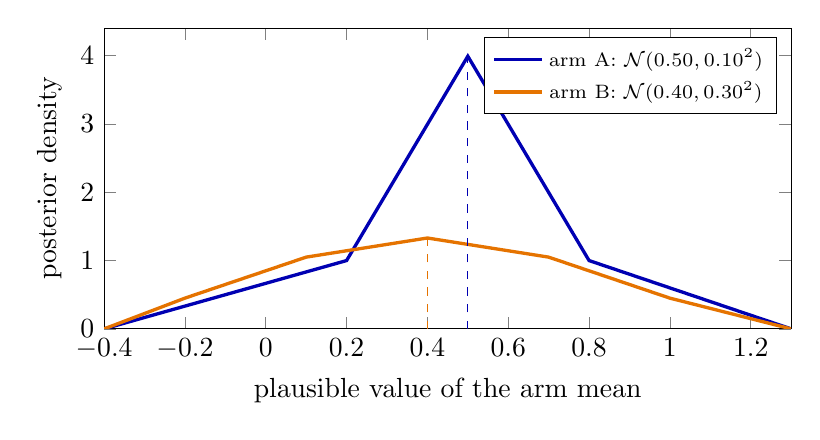
\begin{tikzpicture}
\begin{axis}[width=0.85\linewidth,height=5.4cm,xmin=-0.4,xmax=1.3,ymin=0,ymax=4.4,xlabel={plausible value of the arm mean},ylabel={posterior density},
  no markers,legend style={font=\scriptsize,at={(0.98,0.97)},anchor=north east}]
 \addplot[blue!70!black,very thick] coordinates {(-0.4,0.00) (0.2,1.0) (0.5,3.99) (0.8,1.0) (1.3,0.00)};
 \addplot[orange!90!black,very thick] coordinates {(-0.4,0.00) (-0.2,0.45) (0.1,1.05) (0.4,1.33) (0.7,1.05) (1.0,0.45) (1.3,0.00)};
 \addlegendentry{arm A: $\Norm(0.50,0.10^2)$}
 \addlegendentry{arm B: $\Norm(0.40,0.30^2)$}
 \draw[dashed,blue!70!black] (axis cs:0.5,0) -- (axis cs:0.5,3.99);
 \draw[dashed,orange!90!black] (axis cs:0.4,0) -- (axis cs:0.4,1.33);
\end{axis}
\end{tikzpicture}
\caption{Two posteriors with independent arms. A has the higher mean but B is much more uncertain; B's posterior probability of being the better arm is $\Phi\bigl(-0.1/\sqrt{0.1^2+0.3^2}\bigr)\approx0.376$, so TS plays B about 37.6\% of the time.}
\end{figure}

\begin{intuition}
Why ``sample, then argmax'' (slide 45) is enough: you never compute $\Prob(\text{arm }a\text{ is best})$ explicitly; you just \emph{simulate one possible world} consistent with your beliefs and act optimally in it. Over many rounds the frequency with which each arm wins its
simulated world is precisely its probability of being optimal. In the figure, for independent Gaussians $\Prob(\mu_B>\mu_A)=\Phi\bigl((m_B-m_A)/\sqrt{s_A^2+s_B^2}\bigr)=\Phi(-0.316)\approx0.376$ (a Monte Carlo check with $10^6$ pairs of draws gives $0.375$). The less-known arm keeps getting tried
\emph{in proportion to how plausibly it might be best}; once its posterior narrows below the other arm's, that probability collapses to zero and exploration stops by itself.
\end{intuition}

\subsection{The Gaussian algorithm \slides{46--47}}

\begin{algorithm}[Thompson sampling, Gaussian arms]\label{alg:tsg}
For $t=0,\dots,T$:
\begin{enumerate}
 \item for each arm $i=1,\dots,K$ sample a value $\tilde\mu_t(i)$ \emph{independently} from $\Norm\bigl(\mu_{t-1}(i),\sigma^2_{t-1}(i)\bigr)$ (the slides denote this sampled value by $\hat{\mathbf r}_i$; it is \emph{not} the IPS vector of Section~5);
 \item pull the arm $I_t=\argmax_{i\in[K]}\tilde\mu_t(i)$;
 \item observe the reward $r_t$;
 \item update the posterior of the pulled arm via Corollary~\ref{cor:gauss-step}.
\end{enumerate}
\end{algorithm}

Slide 47 adds two remarks. First, the sampled value is an estimate of the \emph{reward}; in a general MDP it can be replaced by the $Q$-function, i.e.\ we estimate a \emph{distribution over $Q$} and sample from it.
Second, ``this can be done with different distributions as well'' (see Section~\ref{sec:beta}).

\begin{intuition}
Compared with Bayesian UCB, nothing is added to the mean: uncertainty enters \emph{through the randomness of the sample}. A wide posterior occasionally produces a very high draw and so gets tried; a narrow posterior almost always draws close to its mean. This ``randomised optimism''
needs no tuning constant $c$, only a sensible prior.
\end{intuition}

\subsection{Simulation \slides{48}}

\begin{figure}[ht]
\centering
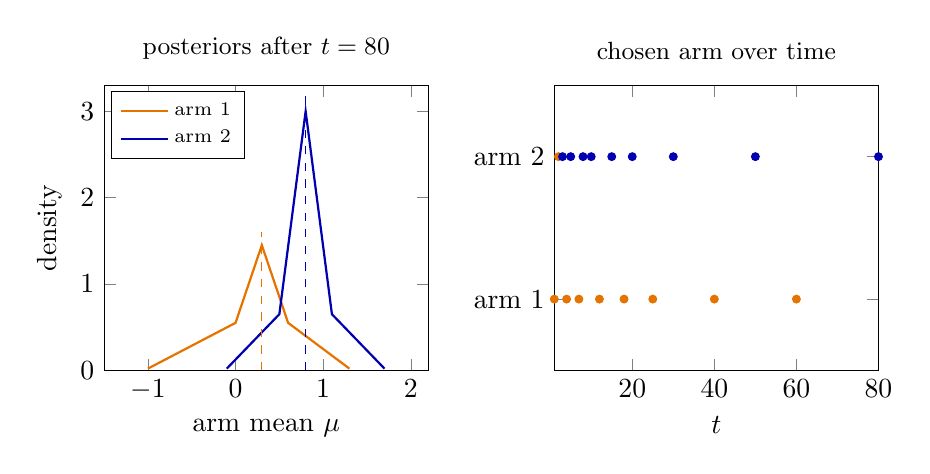
\begin{tikzpicture}
\begin{groupplot}[group style={group size=2 by 1,horizontal sep=1.6cm},width=0.47\linewidth,height=5.2cm,no markers,title style={font=\small}]
 \nextgroupplot[title={posteriors after $t=80$},xlabel={arm mean $\mu$},ylabel={density},xmin=-1.5,xmax=2.2,ymin=0,
   legend style={font=\scriptsize,at={(0.02,0.98)},anchor=north west}]
  \addplot[orange!90!black,thick] coordinates {(-1.0,0.02) (0.0,0.55) (0.3,1.45) (0.6,0.55) (1.3,0.02)};
  \addplot[blue!70!black,thick] coordinates {(-0.1,0.02) (0.5,0.65) (0.8,3.0) (1.1,0.65) (1.7,0.02)};
  \draw[dashed,orange!90!black] (axis cs:0.3,0) -- (axis cs:0.3,1.6);
  \draw[dashed,blue!70!black] (axis cs:0.8,0) -- (axis cs:0.8,3.2);
  \addlegendentry{arm 1}
 \addlegendentry{arm 2}
 \nextgroupplot[title={chosen arm over time},xlabel={$t$},xmin=1,xmax=80,ymin=0.5,ymax=2.5,ytick={1,2},yticklabels={arm 1,arm 2}]
  \addplot[only marks,mark=*,mark size=1.4pt,orange!90!black] coordinates {(1,1) (2,2) (4,1) (7,1) (12,1) (18,1) (25,1) (40,1) (60,1)};
  \addplot[only marks,mark=*,mark size=1.4pt,blue!70!black] coordinates {(3,2) (5,2) (8,2) (10,2) (15,2) (20,2) (30,2) (50,2) (80,2)};
\end{groupplot}
\end{tikzpicture}
\caption{Toy simulation of Algorithm~\ref{alg:tsg} (seeded): two Gaussian arms with true means $0.3$ and $0.8$ (dashed), noise $\sigma=1$, prior $\Norm(0,1)$, $T=80$. Arm~1 is tried 13 times and then largely abandoned; arm~2 is played in 67 rounds.
Final posteriors: arm~1 $\Norm(0.22,0.27^2)$ (still wide, as it was rarely sampled), arm~2 $\Norm(0.69,0.12^2)$ (narrow).}
\end{figure}

% =====================================================================
\section{Bayesian Bandits: Thompson Sampling \slides{49}}\label{sec:beta}

Slide 49 repeats the algorithm with \emph{Beta posteriors} for an A/B ad test (click-through rates in $[0,1]$). Each step: sample $\tilde\theta_A,\tilde\theta_B$ from the Beta posteriors, pick the argmax, observe a click, and update that arm only.

\begin{proposition}[Beta--Bernoulli conjugacy]\label{prop:beta}
If $\mu\sim\mathrm{Beta}(\alpha,\beta)$ and $r\sim\mathrm{Bernoulli}(\mu)$, then $\mu\mid r\sim\mathrm{Beta}(\alpha+r,\ \beta+1-r)$. After $k$ successes in $n$ trials from the uniform prior $\mathrm{Beta}(1,1)$, the posterior is $\mathrm{Beta}(1+k,\,1+n-k)$, with mean $\frac{k+1}{n+2}$ and variance $\frac{\alpha\beta}{(\alpha+\beta)^2(\alpha+\beta+1)}$ (with $\alpha=1+k$, $\beta=1+n-k$).
\end{proposition}
\begin{proof}
The Beta density is proportional to $\mu^{\alpha-1}(1-\mu)^{\beta-1}$ and the Bernoulli likelihood is $\mu^r(1-\mu)^{1-r}$. Their product is proportional to $\mu^{\alpha+r-1}(1-\mu)^{\beta+(1-r)-1}$, the kernel of $\mathrm{Beta}(\alpha+r,\beta+1-r)$.
Iterating $n$ times adds the successes to $\alpha$ and the failures to $\beta$; the moments are those of the Beta distribution.
\end{proof}

\begin{algorithm}[Thompson sampling, Bernoulli rewards]
Keep $(\alpha_i,\beta_i)=(1,1)$ for each arm $i$. At each round: draw $\tilde\theta_i\sim\mathrm{Beta}(\alpha_i,\beta_i)$ for all $i$, play $I_t=\argmax_i\tilde\theta_i$, observe the click $c_t\in\{0,1\}$, and set $\alpha_{I_t}\leftarrow\alpha_{I_t}+c_t$, $\beta_{I_t}\leftarrow\beta_{I_t}+1-c_t$.
\end{algorithm}

\begin{figure}[ht]
\centering
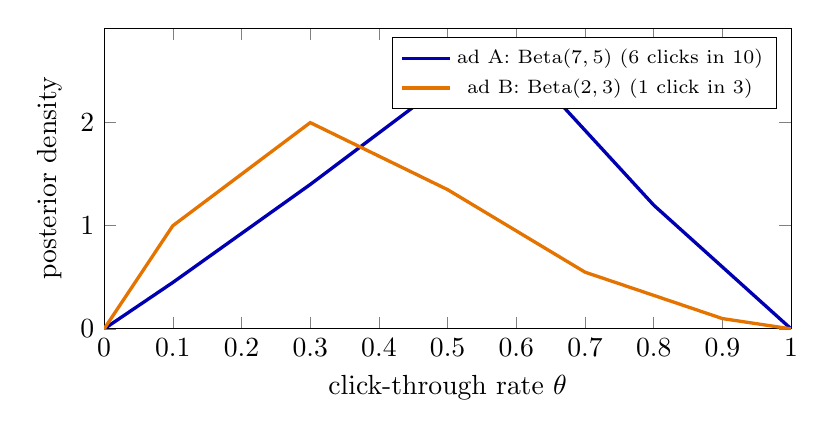
\begin{tikzpicture}
\begin{axis}[width=0.85\linewidth,height=5.4cm,xmin=0,xmax=1,ymin=0,xlabel={click-through rate $\theta$},ylabel={posterior density},no markers,
  legend style={font=\scriptsize,at={(0.98,0.97)},anchor=north east}]
 \addplot[blue!70!black,very thick] coordinates {(0,0) (0.1,0.45) (0.3,1.4) (0.5,2.4) (0.6,2.65) (0.8,1.2) (1,0)};
 \addplot[orange!90!black,very thick] coordinates {(0,0) (0.1,1.0) (0.3,2.0) (0.5,1.35) (0.7,0.55) (0.9,0.1) (1,0)};
 \addlegendentry{ad A: $\mathrm{Beta}(7,5)$ (6 clicks in 10)}
 \addlegendentry{ad B: $\mathrm{Beta}(2,3)$ (1 click in 3)}
\end{axis}
\end{tikzpicture}
\caption{Beta posteriors for an A/B test from the uniform prior (illustrative counts). Ad B has little data, so its posterior is broad.}
\end{figure}

\begin{intuition}
Beta--Bernoulli is the Bernoulli analogue of Proposition~\ref{prop:gauss}: ``pseudo-counts'' of successes and failures. For ad A ($k=6$, $n=10$): mean $7/12\approx0.583$, variance $\approx0.0187$. For ad B ($k=1$, $n=3$): mean $2/5=0.4$, variance $0.04$.
The probability that a draw for A beats a draw for B is $\approx0.77$ (Monte Carlo, $10^6$ draws), so Thompson sampling would show A about 77\% of the time and still B about 23\% of the time, because B's few observations leave
real doubt. Each click or non-click then moves the corresponding posterior and the shares drift towards the truly better ad. This is the ``different distributions'' remark of slides 47 and 49: the algorithm only needs a posterior one can \emph{sample} from.
\end{intuition}

% =====================================================================
\section{Summary}

\begin{table}[ht]
\centering\small
\renewcommand{\arraystretch}{1.25}
\begin{tabular}{>{\raggedright\arraybackslash}p{2.2cm}>{\raggedright\arraybackslash}p{1.35cm}>{\raggedright\arraybackslash}p{3.9cm}>{\raggedright\arraybackslash}p{2.4cm}>{\raggedright\arraybackslash}p{4.05cm}}
\toprule
\textbf{Method} & \textbf{Setting} & \textbf{How it explores} & \textbf{Assumes} & \textbf{Result in this lecture}\\\midrule
Greedy & MAB & try each arm once, commit to the best sample & nothing & linear regret (about $0.08T$ in the Bernoulli example)\\
Explore-then-commit & MAB & $N$ pulls per arm, then commit & rewards in $[0,1]$; needs $T,K,\delta$ to set $N$ & $O(T^{2/3}K^{1/3}\ln^{1/3}(K/\delta))$ (Thm.~\ref{thm:ec-mab})\\
UCB & MAB & optimism: mean $+\sqrt{\ln(KT/\delta)/N_t}$ & rewards in $[0,1]$ & $\widetilde O(\sqrt{KT})$, optimal up to logs (Thm.~\ref{thm:ucb})\\
Explore-then-commit & CB & uniform actions $+$ IPS for $N$ rounds, then $\hat\pi$ & finite $\Pi$ & $O\bigl(T^{2/3}K^{2/3}\ln^{1/3}(|\Pi|/\delta)\bigr)$ as proved (Thm.~\ref{thm:cec}); slide: $K^{1/3}$\\
$\epsilon$-greedy & CB & mixture $(1-\epsilon_t)\delta_{\pi^t}+\epsilon_t\Unif$ $+$ IPS, $\epsilon_t\downarrow0$ & finite/given $\Pi$ & no bound stated (simulation only)\\
Bayesian UCB & MAB (Gaussian) & posterior mean $+\,c\,\sigma_t/\sqrt{N_t}$ & Gaussian prior and noise & none stated (rule and snapshot)\\
Thompson sampling & MAB / CB & sample from posterior, act greedily on the sample & sampleable posterior (Gaussian, Beta, \dots) & plays arm $a$ with prob.\ $\Prob(a\text{ optimal})$ (Prop.~\ref{prop:pm}); no regret bound stated\\\bottomrule
\end{tabular}
\caption{Comparison of the methods covered. ``CB'' = contextual bandit, ``MAB'' = multi-armed bandit. ``None stated'' means neither the slides nor the companion note give a bound.}
\end{table}

\begin{figure}[ht]
\centering
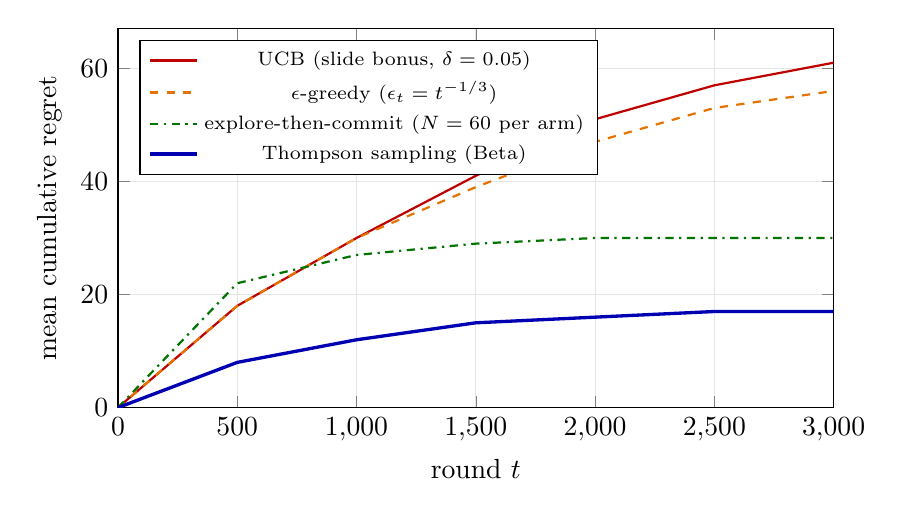
\begin{tikzpicture}
\begin{axis}[width=0.88\linewidth,height=6.4cm,xlabel={round $t$},ylabel={mean cumulative regret},xmin=0,xmax=3000,ymin=0,no markers,
  legend style={font=\scriptsize,at={(0.03,0.97)},anchor=north west},grid=both,grid style={black!10}]
 \addplot[red!75!black,thick] coordinates {(0,0) (500,18) (1000,30) (1500,41) (2000,51) (2500,57) (3000,61)};
 \addplot[orange!90!black,thick,dashed] coordinates {(0,0) (500,18) (1000,30) (1500,39) (2000,47) (2500,53) (3000,56)};
 \addplot[green!45!black,thick,dash dot] coordinates {(0,0) (500,22) (1000,27) (1500,29) (2000,30) (2500,30) (3000,30)};
 \addplot[blue!70!black,very thick] coordinates {(0,0) (500,8) (1000,12) (1500,15) (2000,16) (2500,17) (3000,17)};
 \addlegendentry{UCB (slide bonus, $\delta=0.05$)}
 \addlegendentry{$\epsilon$-greedy ($\epsilon_t=t^{-1/3}$)}
 \addlegendentry{explore-then-commit ($N=60$ per arm)}
 \addlegendentry{Thompson sampling (Beta)}
\end{axis}
\end{tikzpicture}
\caption{Toy simulation (qualitative): Bernoulli bandit with $K=3$ arms of means $0.7,0.5,0.4$, $T=3000$, regret averaged over 300 seeded runs. At $T=3000$ the average regrets are about $17$ (Thompson), $30$ (explore-then-commit), $56$ ($\epsilon$-greedy) and $61$ (UCB).
Constants matter in a short horizon: UCB with the conservative slide bonus $\sqrt{\ln(KT/\delta)/N}$ explores a lot, and explore-then-commit works well here only because $N=60$ was hand-picked (the theory needs the gaps, or $T,K,\delta$ and a bound, to choose it).
Asymptotically the ordering of \emph{rates} (linear $\gg T^{2/3}\gg\sqrt T$) is what the theorems describe.}
\end{figure}

\subsection*{Key take-aways}
\begin{itemize}
 \item \textbf{Exploration is unavoidable, and regret measures its price.} Greedy suffers linear regret; explore-then-commit balances exploration against commitment to get $T^{2/3}$; optimism (UCB) gets the optimal $\sqrt T$ rate up to logs, with no schedule to tune.
 \item \textbf{Context changes the object being learned, not the logic.} A contextual bandit asks for a \emph{policy}, with i.i.d.\ contexts and bandit feedback; regret is measured against the best policy in $\Pi$, and the cost of a rich class is only $\ln|\Pi|$ (inside a cube root).
 \item \textbf{IPS makes learning from partial feedback possible.} Dividing by the known propensity gives an unbiased estimate of every action's reward (Lemma~\ref{lem:ips}), at the price of variance up to $K$ (uniform exploration) or $K/\epsilon_t$ ($\epsilon$-greedy), which is why exploration probabilities must stay positive.
 \item \textbf{Explore-then-commit separates the phases, $\epsilon$-greedy interleaves them.} The first is easy to analyse (Theorem~\ref{thm:cec}); the second keeps learning and adapting but needs a decay schedule for $\epsilon_t$.
 \item \textbf{Bayesian bandits turn uncertainty into a distribution you can use.} Conjugate updates (Gaussian, Beta--Bernoulli) are one-line formulas; Bayesian UCB adds a multiple of the posterior width, while Thompson sampling samples from the posterior and thereby plays each arm with its probability of being optimal (Proposition~\ref{prop:pm}).
\end{itemize}

% =====================================================================
\appendix
\section{Supplementary material (in the companion note, not on the slides)}\label{app:supp}

The following result is in the companion note but has no corresponding slide; it supplies the technical ingredient (range of the IPS terms) used in the proof of Theorem~\ref{thm:cec}.

\begin{lemma}[What unbiasedness costs]\label{lem:range}
Under uniform exploration, $0\le\rh_t[a]\le K$ and $\Var\bigl(\rh_t[a]\mid x_t\bigr)\le K$.
\end{lemma}
\begin{proof}
The estimator is $Kr_t\le K$ on one action and $0$ elsewhere, which gives the range. For the variance,
$\E[\rh_t[a]^2\mid x_t]=\frac1K\,K^2\,\E[r_t^2\mid x_t,a]\le K$, since rewards lie in $[0,1]$, and the variance is at most the second moment.
\end{proof}

\begin{intuition}
Unbiasedness is bought with noise: each observation is $0$ with probability $1-1/K$ and $Kr_t$ with probability $1/K$. With $K=10$ actions and reward $0.5$, a single IPS observation is either $0$ or $5$ although the target is $0.5$; its variance is $10\cdot0.25-0.25=2.25$, versus at most $0.25$ for a $[0,1]$-valued observation.
The \emph{range} bound $K$ is what Hoeffding's inequality uses in Theorem~\ref{thm:cec}; the \emph{variance} bound $K$ is what Bernstein's inequality would use to sharpen the dependence on $K$ (see the remark after that theorem).
\end{intuition}

\section{Notation map and slide/note discrepancies}\label{app:notes}

\begin{table}[ht]
\centering\small
\renewcommand{\arraystretch}{1.2}
\begin{tabular}{lll}\toprule
\textbf{Concept} & \textbf{Slides} & \textbf{Companion note / these notes}\\\midrule
context, context set & $x_t$, $\mathcal X$ & $z_t$, $\mathcal Z$ $\;/\;$ $x_t$, $\calX$\\
context distribution & $\mu$ & $\rho$\\
action at round $t$ & $a_t$ (CB), $I_t$ (MAB) & $A_t$ $\;/\;$ $a_t$, $I_t$\\
policy at round $t$ & $\pi^t$ & $\pi_t$\\
regret & $\mathrm{Regret}_T$ & $\mathrm{Reg}(T)$\\
IPS vector & $\hat{\mathbf r}_t[a]$ & $\hat r_t[a]$ $\;/\;$ $\rh_t[a]$\\\bottomrule
\end{tabular}
\end{table}

Small inconsistencies noticed while merging the two sources, and how these notes treat them:
\begin{itemize}
 \item \textbf{Slide 8:} ``Set $N=T/K$'' would use all $T$ rounds for exploration; read it as a placeholder with $NK\ll T$. The optimised $N^\star$ is on slide 12 and in Theorem~\ref{thm:ec-mab}.
 \item \textbf{Slide 12:} ``approaches 0 as $T$ goes to infinity'' refers to the \emph{average} regret $\Reg_T/T\sim T^{-1/3}$; the regret itself grows (sub-linearly).
 \item \textbf{Slides 11--12 and 14:} confidence widths are written with $\ln(K/\delta)$ or $\ln(KT/\delta)$, hiding the constant $2$ and Hoeffding's factor $\tfrac12$ inside $O(\cdot)$; the proofs here keep $\ln(2K/\delta)$ and $\ln(2KT/\delta)$.
 \item \textbf{Slide 31 vs.\ Theorem~\ref{thm:cec}:} slide $K^{1/3}$, proved bound $K^{2/3}$; see the remark after the theorem.
 \item \textbf{Slide 42:} ``highest standard deviation'' should read ``highest mean plus $c$ standard errors'', as the displayed formula says.
 \item \textbf{Slides 46--47:} the hat-bold-$r$ symbol there denotes a \emph{sample from the posterior}, unrelated to the IPS vector of slides 27--35.
 \item \textbf{Slide 40:} the recursive update is written with the likelihood evaluated at the current posterior parameters; the closed form is Corollary~\ref{cor:gauss-step}.
\end{itemize}

\newpage

% ======================================================================
% Lecture 2 -- Part 2
% ======================================================================
\part{Lecture 2 -- Part 2}

\begin{center}\small
Structure follows the slide deck (slides 1--55); formal statements and proofs are merged in from the
companion PDF at the point where the slides introduce the topic. Material that appears only in the PDF is
collected in the Appendix.
\end{center}

\bigskip

%=====================================================================
\section{Recap \slr{2--11}}
%=====================================================================
The lecture opens by recalling the bandit material of the previous lectures (slide 2 opens the recap, slide 11 closes it). The point of the recap is to set up the jump from \emph{one-step} decision making to \emph{sequential} decision making.

\subsection{From Multi-Armed to Contextual Bandits \slr{3}}
A multi-armed bandit (MAB) is stateless: the agent picks an action and receives a reward. A \emph{contextual bandit} (CB) adds back some context (a state): before acting, the agent sees a context $x_t$, and the reward depends on both the context and the arm.

\begin{figure}[htbp]
\centering
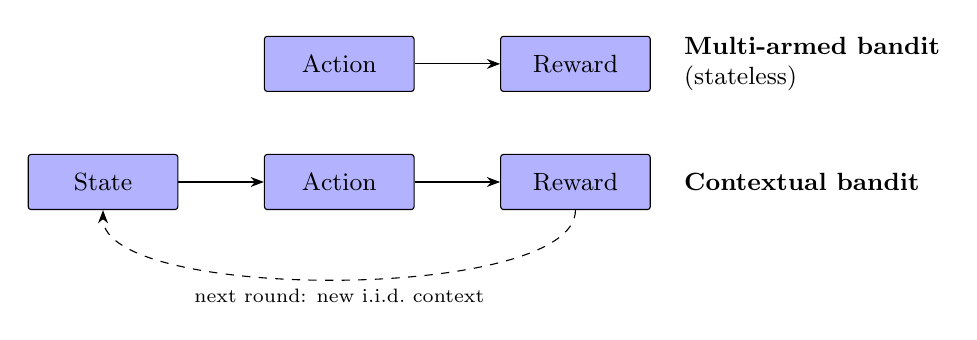
\begin{tikzpicture}[>=Stealth,
  box/.style={draw,fill=blue!30,rounded corners=1pt,minimum width=1.9cm,minimum height=0.7cm,font=\small}]
  \node[box] (a1) at (0,1.5) {Action};
  \node[box] (r1) at (3,1.5) {Reward};
  \draw[->] (a1)--(r1);
  \node[anchor=west,align=left,font=\small] at ([xshift=3mm]r1.east) {\textbf{Multi-armed bandit}\\(stateless)};
  \node[box] (s2) at (-3,0) {State};
  \node[box] (a2) at (0,0) {Action};
  \node[box] (r2) at (3,0) {Reward};
  \draw[->] (s2)--(a2); \draw[->] (a2)--(r2);
  \node[anchor=west,align=left,font=\small] at ([xshift=3mm]r2.east) {\textbf{Contextual bandit}};
  \draw[->,dashed] (r2.south) to[out=-90,in=-90,looseness=0.5]
     node[below,font=\scriptsize]{next round: new i.i.d.\ context} (s2.south);
\end{tikzpicture}
\caption{MAB versus contextual bandit (redrawn from slide 3).}
\end{figure}

\begin{intuition}
Think of a MAB as a single slot machine room with no information about who walks in; a CB is the same room where each customer has a profile $x_t$ and the best machine depends on the profile. The crucial point for what follows: in a CB the context is drawn i.i.d., so \emph{my action does not change the next context}. MDPs remove exactly this restriction.
\end{intuition}

\subsection{Contextual Bandits: Interaction \slr{4}}
For $t=0,\dots,T-1$:
\begin{enumerate}[nosep]
  \item a new i.i.d.\ context $x_t\in\mathcal X$ appears;
  \item select an action $a_t\in\cA$ based on historical information and the context;
  \item observe the reward $r(x_t,a_t)$ (context- and arm-dependent).
\end{enumerate}
For simplicity the rewards are assumed deterministic, ``as the context is the challenge here''.

\subsection{Contextual Bandits: Regret \slr{5}}
The optimal policy is $\pi^\star=\argmax_{\pi\in\Pi}\E_{x\sim\mu}[r(x,\pi(x))]$. At every iteration $a_t=\pi^t(x_t)$ is chosen, and the regret compares the total expected reward of always using $\pi^\star$ with that of our learned sequence of policies:
\[
  \mathrm{Regret}_T \;=\; T\,\E_{x\sim\mu}\!\left[r(x,\pi^\star(x))\right]\;-\;\sum_{t=0}^{T-1}\E_{x\sim\mu}\!\left[r(x,\pi^t(x))\right].
\]
Note that the policies $\pi^t$ are different at every iteration $t$.

\begin{intuition}
Regret is ``how much reward I left on the table by not knowing $\pi^\star$ from day one''. If $\mathrm{Regret}_T$ grows sublinearly in $T$, the \emph{average} regret per round goes to $0$: eventually the learner behaves like the optimal policy.
\end{intuition}

\subsection{Explore \& Commit Algorithm \slr{6}}
\begin{algorithm}[Explore \& Commit for contextual bandits]
\begin{enumerate}[nosep]
  \item For $t=0,\dots,N-1$ (\emph{explore}): observe $x_t\sim\mu$; sample $a_t\sim\mathrm{Unif}(\cA)$; observe $r_t=r(x_t,a_t)$; build, for $x_t$, an unbiased estimate $\hat r_t$ of the reward vector, with $\E_{a_t\sim\mathrm{Unif}(\cA)}\hat r_t[a]=r(x_t,a)\ \forall a$:
  \[
   \hat r_t[a]=\begin{cases}0 & a\neq a_t\\[2pt] \dfrac{r_t}{1/|\cA|} & a=a_t.\end{cases}
  \]
  \item Compute the policy $\hat\pi=\argmax_{\pi\in\Pi}\sum_{t=0}^{N-1}\hat r_t[\pi(x_t)]$.
  \item For $t=N,\dots,T-1$ (\emph{commit}): observe $x_t\sim\mu$ and play $a_t=\hat\pi(x_t)$.
\end{enumerate}
\end{algorithm}
With a suitable $N$ the regret is
\[
  \mathrm{Regret}_T=O\!\left(T^{2/3}K^{1/3}\ln(|\Pi|)^{1/3}\right),\qquad K=|\cA|.
\]

\begin{intuition}
The division by $1/|\cA|$ is \emph{importance weighting}: we only see the reward of the arm we actually played, which happens with probability $1/|\cA|$, so we inflate it by $|\cA|$ to be right on average. A numerical feel for the rate: doubling the horizon multiplies the regret bound by only $2^{2/3}\approx1.59$, so the per-round regret decays like $T^{-1/3}$.
\end{intuition}

\subsection{\texorpdfstring{$\epsilon$}{epsilon}-Greedy \slr{7}}
Instead of fixing a threshold for exploring and then committing, interleave exploration and exploitation. For $t=0,\dots,T$: observe $x_t\sim\mu$; draw
\[
  a_t\sim p_t=(1-\epsilon)\,\delta\big(\pi^t(x_t)\big)+\epsilon\,\mathrm{Unif}(\cA);
\]
observe $r_t=r(x_t,a_t)$; build an unbiased estimate $\hat r_t$ for $x_t$ (so that $\E_{a\sim p_t}\hat r_t[a]=r(x_t,a)$); update the policy $\pi^{t+1}=\argmax_{\pi\in\Pi}\sum_{\tau\le t}\hat r_\tau[\pi(x_\tau)]$. Here $\epsilon=0$ means pure exploitation and $\epsilon=1$ uniform exploration. (The slide only asserts unbiasedness; the usual choice is the importance-weighted estimator $\hat r_t[a]=\mathbb 1[a=a_t]\,r_t/p_t(a_t)$.)

\begin{intuition}
Explore \& Commit explores first, then stops learning. $\epsilon$-greedy never stops: with $\epsilon=0.1$, about one round in ten is a random experiment, and the other nine use the current best guess. It is robust to the case where the early estimates were wrong.
\end{intuition}

\subsection{Bayesian Bandits \slr{8}}
So far no assumption was made about the reward distributions $\nu_i$; only bounds on rewards were derived. In Bayesian bandits we (i) exploit \emph{prior} knowledge of rewards, (ii) update a \emph{posterior} distribution from historical information, and (iii) use the posterior to guide exploration, either through upper confidence bounds (Bayesian UCB) or probability matching (Thompson sampling).

\subsection{Gaussian Bayesian Bandits: UCB \slr{9}}
Now that a distribution is modelled, a notion of confidence comes for free: for Gaussians it is the standard deviation. The UCB rule picks
\[
  a_t=\argmax_{i\in K}\;\mu_t(i)+\frac{c\,\sigma_t(i)}{\sqrt{N_t(i)}},
\]
where $N_t(i)$ is the number of pulls of arm $i$ and $c$ a constant.

\subsection{Gaussian Bayesian Bandits: Thompson Sampling \slr{10}}
For $t=0,\dots,T$: for each arm $i=1,\dots,K$ sample $\tilde r_t(i)$ independently from $\mathcal N(\mu_{t-1}(i),\sigma^2_{t-1}(i))$; pull $I_t=\argmax_i\tilde r_t(i)$; observe $r_t$; update the posterior $p(\mu_t(i),\sigma_t^2(i)\mid r_t)$. This can be done with other distributions as well. The slide stresses that this is an estimate of the \emph{reward}: in more general MDPs it is replaced by the $Q$ function, i.e.\ we estimate a distribution over $Q$.

\begin{figure}[htbp]
\centering
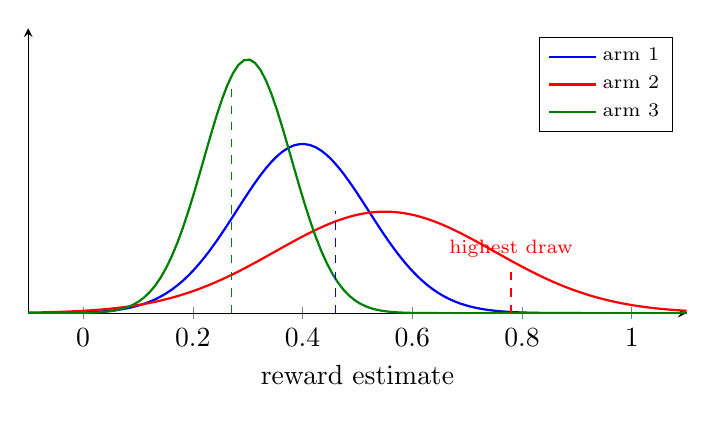
\begin{tikzpicture}
\begin{axis}[width=0.82\linewidth,height=5.2cm,xlabel={reward estimate},ytick=\empty,
  axis lines=left,legend style={font=\scriptsize,at={(0.98,0.97)},anchor=north east},
  domain=-0.1:1.1,samples=120,ymin=0,ymax=5.6]
 \addplot[blue,thick]{exp(-0.5*((x-0.40)/0.12)^2)/(0.12*2.5066)};
 \addplot[red,thick]{exp(-0.5*((x-0.55)/0.20)^2)/(0.20*2.5066)};
 \addplot[green!50!black,thick]{exp(-0.5*((x-0.30)/0.08)^2)/(0.08*2.5066)};
 \legend{arm 1,arm 2,arm 3}
 \addplot[blue,dashed] coordinates{(0.46,0)(0.46,2.0)};
 \addplot[red,dashed] coordinates{(0.78,0)(0.78,0.8)};
 \addplot[green!50!black,dashed] coordinates{(0.27,0)(0.27,4.5)};
 \node[red,font=\scriptsize,anchor=south] at (axis cs:0.78,0.9) {highest draw};
\end{axis}
\end{tikzpicture}
\caption{Thompson sampling with Gaussian posteriors (original illustration of the idea on slide 10; the numbers are illustrative). Dashed lines are the independent draws $\tilde r(i)$; the uncertain arm~2 gets the highest draw and is pulled.}
\end{figure}

\begin{intuition}
Thompson sampling explores in proportion to uncertainty without any explicit exploration parameter: an arm with a wide posterior occasionally produces a high draw and gets tried; once its posterior narrows and its mean is low, the draws stop beating the others. This is the ``probability matching'' idea: pull each arm with the probability that it is the best.
\end{intuition}

%=====================================================================
\section{Sequential Decision Making \slr{12--14}}
%=====================================================================
The agent interacts with the environment at discrete time steps, by receiving an observation $o_t$ and a reward $r_t$ from the environment and by taking actions $a_t$ (slide 12).

\begin{figure}[htbp]
\centering
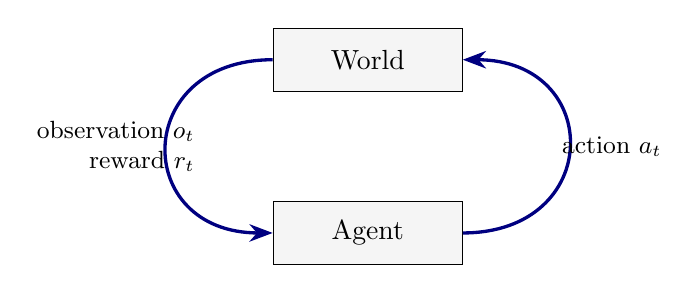
\begin{tikzpicture}[>=Stealth,
  box/.style={draw,minimum width=2.4cm,minimum height=0.8cm,fill=gray!8}]
  \node[box] (w) at (0,2.2) {World};
  \node[box] (ag) at (0,0) {Agent};
  \draw[->,very thick,blue!50!black] (w.west) .. controls (-3,2.2) and (-3,0) .. (ag.west);
  \draw[->,very thick,blue!50!black] (ag.east) .. controls (3,0) and (3,2.2) .. (w.east);
  \node[align=right,font=\small] at (-3.2,1.1) {observation $o_t$\\ reward $r_t$};
  \node[font=\small] at (3.1,1.1) {action $a_t$};
\end{tikzpicture}
\caption{The agent--world loop (slides 12--14, redrawn).}
\end{figure}

Such a discrete interaction generates a trajectory, or \emph{history}, at each time step $t$, which the agent uses to choose its action (slide 13):
\[
  h_t=(o_0,a_0,r_1,o_1,a_1,\dots,r_t,o_t,a_t)\quad\text{(indexing convention as on the slide)}.
\]
The \emph{state} is a function of the history, $s_t=f(h_t)$, and it is typically hidden or unknown (slide 14).

\begin{intuition}
The history grows without bound; no practical agent can condition on all of it. The state is a \emph{summary} of the history that is supposed to keep what matters for the future. Which summary is a good one is exactly the question the Markov assumption answers.
\end{intuition}

%=====================================================================
\section{Markov Assumption \slr{15--17}}
%=====================================================================
\begin{definition}[Markov state]\label{def:markov}
A state representation is Markov if for every $t$, every history $h_t$ and every action $a_t$,
\[
  p(s_{t+1}\mid s_t,a_t)=p(s_{t+1}\mid h_t,a_t).
\]
The future is conditionally independent of the past given the present.
\end{definition}

\begin{intuition}
If I tell you the current state and my action, nothing in the earlier history can sharpen your prediction of the next state. A chess position is Markov (how we reached it is irrelevant for what can happen next). The position of a moving ball alone is \emph{not}: without its velocity, the past positions carry extra information.
\end{intuition}

\begin{figure}[H]
	\centering
	\includegraphics[width=1.0\linewidth]{1790936412217.png}
	\caption{Is this problem Markovian?}\label{fig:1790936412217}
\end{figure}
Slide 16 asks, over a picture of a robot in a corridor with two pillars, ``Is this problem Markovian?'' The answer depends on what we put in the state: if the state is only the robot's position but the dynamics depend on, e.g., its velocity or an unobserved internal variable, past observations help predict the future and the state is \emph{not} Markov; adding the missing variables restores the property.


Slide 17 gives the two extremes:
\begin{itemize}[nosep]
  \item a state can \emph{always} be made Markov by taking it equal to the whole history, $s_t=h_t$;
  \item the best case, used in practice, is that the state is (a sufficient statistic of) the latest observation, $s_t=o_t$. The state is then said to be \emph{fully observable}.
\end{itemize}

\begin{figure}[htbp]
\centering
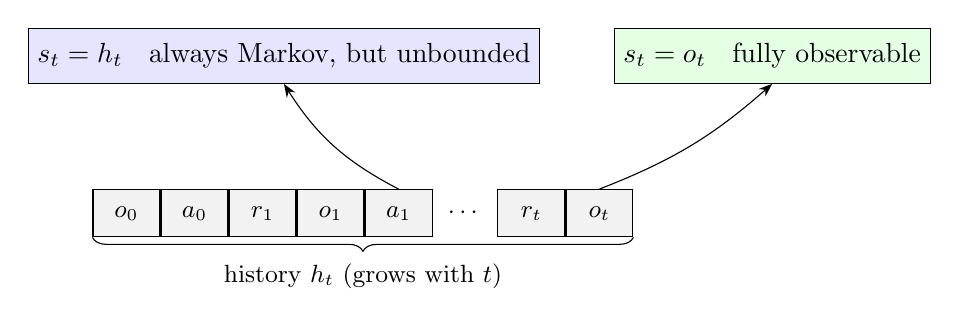
\begin{tikzpicture}[>=Stealth,
  it/.style={draw,minimum width=0.85cm,minimum height=0.6cm,font=\small,fill=gray!10}]
  \node[it](o0)at(0,0){$o_0$};\node[it,right=0pt of o0](a0){$a_0$};
  \node[it,right=0pt of a0](r1){$r_1$};\node[it,right=0pt of r1](o1){$o_1$};
  \node[it,right=0pt of o1](a1){$a_1$};\node[right=2pt of a1,font=\small](dd){$\cdots$};
  \node[it,right=2pt of dd](rt){$r_t$};\node[it,right=0pt of rt](ot){$o_t$};
  \draw[decorate,decoration={brace,mirror,amplitude=5pt}] (o0.south west)--(ot.south east)
     node[midway,below=6pt,font=\small]{history $h_t$ (grows with $t$)};
  \node[draw,fill=blue!10,minimum height=0.7cm] (s1) at (2,2) {$s_t=h_t$ \; always Markov, but unbounded};
  \node[draw,fill=green!10,minimum height=0.7cm] (s2) at (8.2,2) {$s_t=o_t$ \; fully observable};
  \draw[->] (a1.north) to[bend left=15] (s1.south);
  \draw[->] (ot.north) to[bend right=10] (s2.south);
\end{tikzpicture}
\caption{Two extreme choices of state as a function of the history (original illustration of slide 17).}
\end{figure}

\begin{intuition}
Choosing $s_t=h_t$ is a cheat: it is trivially Markov, but the state space explodes with time. Practical RL wants a small state that is still Markov. Fully observable means the observation already contains everything relevant; this is the setting of the rest of the lecture.
\end{intuition}

%=====================================================================
\section{Markov Decision Process (MDP) \slr{18--19}}
%=====================================================================
An MDP is sequential decision making under the Markov assumption: Markovian transition dynamics, full observability, and a (generally) stochastic transition kernel $p(s_{t+1}\mid s_t,a_t)$. Alternative notation: $s_{t+1}\sim p(\cdot\mid s_t,a_t)$ or $s'\sim p(\cdot\mid s,a)$ (slide 19).

\begin{definition}[Markov decision process]\label{def:mdp}
A discounted infinite-horizon MDP is a tuple $(\cS,\cA,p,r,\gamma)$: a set of states, a set of actions, transition dynamics $p(s'\mid s,a)$ satisfying Definition~\ref{def:markov}, a reward function $r:\cS\times\cA\to[0,\Rmax]$, and a discount factor $\gamma\in[0,1)$. Unless stated otherwise $\cS$ and $\cA$ are finite.
\end{definition}
(The slides introduce $\gamma$ later, in the ``Infinite Horizon Discounted Setting'' part; the tuple is stated here in full for reference.)

\begin{figure}[htbp]
\centering
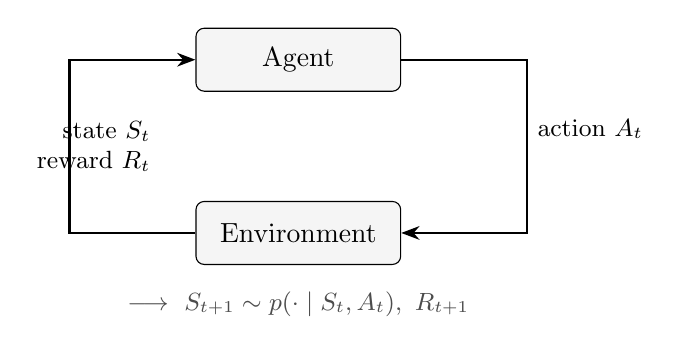
\begin{tikzpicture}[>=Stealth,
  box/.style={draw,rounded corners=3pt,minimum width=2.6cm,minimum height=0.8cm,fill=gray!8}]
  \node[box](ag) at (0,2.2){Agent};
  \node[box](en) at (0,0){Environment};
  \draw[->,thick] (ag.east) -- ++(1.6,0) |- node[pos=0.2,right,font=\small]{action $A_t$} (en.east);
  \draw[->,thick] (en.west) -- ++(-1.6,0.0) |- (ag.west);
  \node[align=right,font=\small] at (-2.6,1.1){state $S_t$\\ reward $R_t$};
  \node[font=\small,gray!60!black] at (0,-0.9){$\longrightarrow\ S_{t+1}\sim p(\cdot\mid S_t,A_t),\ R_{t+1}$};
\end{tikzpicture}
\caption{The MDP interaction loop (slides 18--19, redrawn).}
\end{figure}

\begin{intuition}
An MDP is the contextual bandit \emph{with consequences}: the next ``context'' is the next state $s'$, and it is drawn from a distribution that depends on the action just taken. Every action therefore has two effects: the reward now, and the situation in which the next decision is made.
\end{intuition}

%=====================================================================
\section{Reward \slr{20}}
%=====================================================================
A reward $r_t$ is a scalar signal representing feedback and indicating how well the agent is doing at step $t$. It is a function of state and action, written $r(s,a)$ (sometimes $r(s',a,s)$). A \emph{cost} is the negative of a reward.

\emph{Reward hypothesis} (slide 20, flagged as an open question): can all goals be achieved through the maximisation of a numerical reward?

\begin{intuition}
The reward is the only way we tell the agent what we want; everything else (what is a good state, a good action) must be \emph{derived} from it. That is why designing rewards is delicate: the agent maximises what we write, not what we meant.
\end{intuition}

%=====================================================================
\section{Deterministic MDP Example \slr{21}}
%=====================================================================
The slide shows a small deterministic MDP of a developer's day: states \emph{Wake Up} ($r=0$), \emph{Netflix} ($r=-2$, with a self-loop), \emph{Code \& Debug} ($r=-3$), \emph{Nap} ($r=1$), \emph{Deploy} ($r=10$) and \emph{Sleep} ($r=3$, terminal).

\begin{figure}[htbp]
\centering
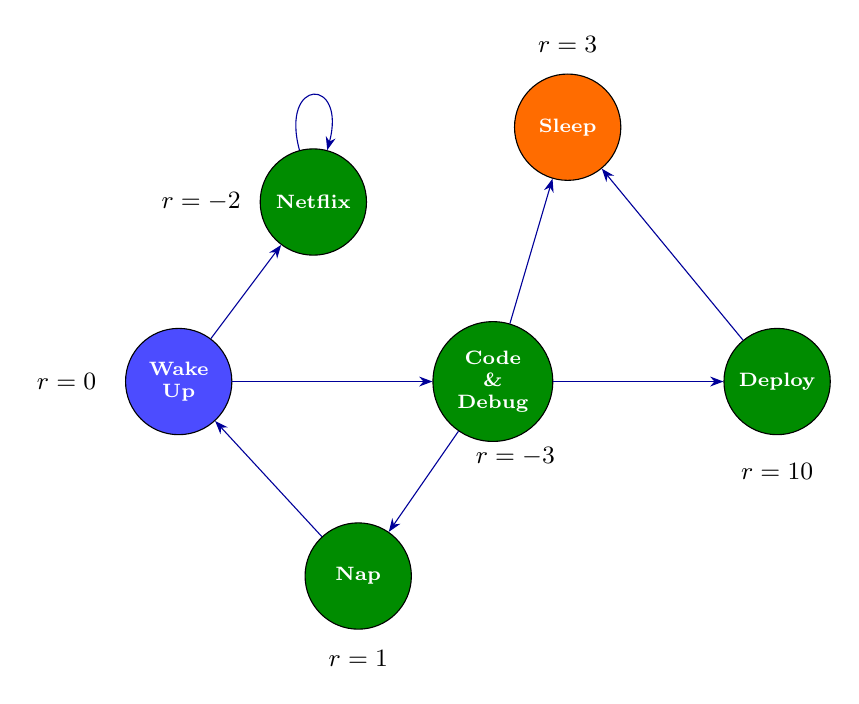
\begin{tikzpicture}[>=Stealth,scale=0.95,
  st/.style={circle,draw,minimum size=1.35cm,font=\scriptsize\bfseries,align=center,text=white,fill=green!55!black}]
  \node[st,fill=blue!70](wk) at (0,0){Wake\\Up};
  \node[st](nf) at (1.8,2.4){Netflix};
  \node[st](cd) at (4.2,0){Code\\\&\\Debug};
  \node[st,fill=orange!85!red](sl) at (5.2,3.4){Sleep};
  \node[st](dp) at (8,0){Deploy};
  \node[st](np) at (2.4,-2.6){Nap};
  \draw[->,blue!60!black] (wk)--(nf);
  \draw[->,blue!60!black] (wk)--(cd);
  \draw[->,blue!60!black] (nf) to[loop above,looseness=7] (nf);
  \draw[->,blue!60!black] (cd)--(sl);
  \draw[->,blue!60!black] (cd)--(dp);
  \draw[->,blue!60!black] (cd)--(np);
  \draw[->,blue!60!black] (np)--(wk);
  \draw[->,blue!60!black] (dp)--(sl);
  \node[font=\small] at (-1.5,0){$r=0$};
  \node[font=\small] at (0.3,2.4){$r=-2$};
  \node[font=\small] at (4.5,-1.0){$r=-3$};
  \node[font=\small] at (5.2,4.5){$r=3$};
  \node[font=\small] at (8,-1.2){$r=10$};
  \node[font=\small] at (2.4,-3.7){$r=1$};
\end{tikzpicture}
\caption{The deterministic MDP of slide 21, redrawn. Rewards are attached to states.}
\end{figure}

\begin{example}[Worked numbers, not on the slide]
Take $\gamma=0.9$, collect the reward of a state when leaving it, and treat Sleep as terminal (its reward is collected once). Then:
\begin{itemize}[nosep]
 \item $V(\text{Sleep})=3$, $V(\text{Deploy})=10+0.9\cdot3=12.7$, $V(\text{Netflix})=-2/(1-0.9)=-20$ (it can only loop).
 \item From Code \& Debug: $Q(\text{Code},\text{Deploy})=-3+0.9\cdot12.7=8.43$, $Q(\text{Code},\text{Sleep})=-3+0.9\cdot3=-0.3$. The best choice is Deploy: a ``bad'' step (reward $-3$) pays off.
 \item Hence the path Wake$\to$Code$\to$Deploy$\to$Sleep has discounted return $0+0.9\cdot8.43=7.587$, while Wake$\to$Netflix forever has return $0+0.9\cdot(-20)=-18$.
 \item Going Code$\to$Nap$\to$Wake gives $V(\text{Nap})=1+0.9\cdot7.587\approx7.83$ and $Q(\text{Code},\text{Nap})\approx4.05<8.43$, so Nap loses.
\end{itemize}
\end{example}

\begin{intuition}
The immediate reward at Code \& Debug is negative ($-3$), yet it is the right place to go through: all the value sits behind it (Deploy $=10$). A myopic agent at Wake Up compares $-2$ (Netflix) with $-3$ (Code \& Debug) and picks Netflix, where it is stuck forever with value $-20$; maximising the \emph{return} sends it through Code \& Debug instead. This is the entire reason we define value functions.
\end{intuition}

%=====================================================================
\section{Stochastic MDP Example \slr{22}}
%=====================================================================
The slide (taken from Sutton \& Barto) shows the \emph{recycling robot}: states \texttt{high} and \texttt{low} battery; actions \texttt{search}, \texttt{wait}, \texttt{recharge}. The transition table of the slide is:
\begin{center}
\renewcommand{\arraystretch}{1.15}
\begin{tabular}{llllc}
\toprule
$s$ & $a$ & $s'$ & $p(s'\mid s,a)$ & $r(s,a,s')$\\
\midrule
high & search   & high & $\alpha$   & $r_{\text{search}}$\\
high & search   & low  & $1-\alpha$ & $r_{\text{search}}$\\
low  & search   & high & $1-\beta$  & $-3$\\
low  & search   & low  & $\beta$    & $r_{\text{search}}$\\
high & wait     & high & $1$        & $r_{\text{wait}}$\\
high & wait     & low  & $0$        & --\\
low  & wait     & high & $0$        & --\\
low  & wait     & low  & $1$        & $r_{\text{wait}}$\\
low  & recharge & high & $1$        & $0$\\
low  & recharge & low  & $0$        & --\\
\bottomrule
\end{tabular}
\end{center}

\begin{figure}[htbp]
\centering
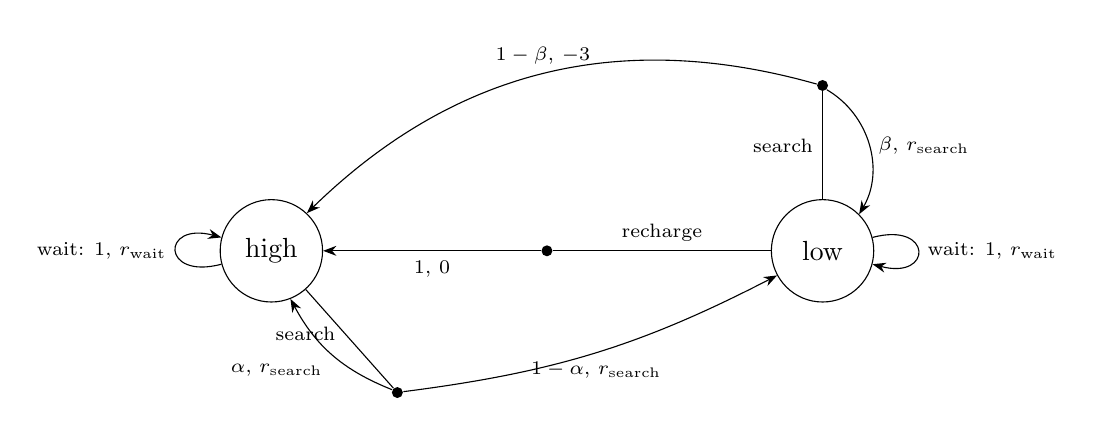
\begin{tikzpicture}[>=Stealth,
  st/.style={circle,draw,minimum size=1.3cm},
  ac/.style={circle,fill=black,inner sep=1.4pt}]
  \node[st](hi) at (0,0){high};
  \node[st](lo) at (7,0){low};
  \path (hi) edge[->,loop left,looseness=6] node[left,font=\scriptsize]{wait: $1,\,r_{\text{wait}}$} (hi);
  \path (lo) edge[->,loop right,looseness=6] node[right,font=\scriptsize]{wait: $1,\,r_{\text{wait}}$} (lo);
  % search from high
  \node[ac](sh) at (1.6,-1.8){};
  \draw (hi)--(sh) node[pos=0.45,left,font=\scriptsize]{search};
  \draw[->] (sh) to[bend left=20] node[pos=0.5,below left,font=\scriptsize]{$\alpha,\,r_{\text{search}}$} (hi);
  \draw[->] (sh) to[bend right=10] node[below,font=\scriptsize]{$1-\alpha,\,r_{\text{search}}$} (lo);
  % search from low
  \node[ac](sl) at (7,2.1){};
  \draw (lo)--(sl) node[pos=0.5,left,font=\scriptsize]{search};
  \draw[->] (sl) to[bend left=45] node[right,font=\scriptsize]{$\beta,\,r_{\text{search}}$} (lo);
  \draw[->] (sl) to[bend right=30] node[above,font=\scriptsize]{$1-\beta,\,-3$} (hi);
  % recharge
  \node[ac](rc) at (3.5,0){};
  \draw (lo)--(rc) node[pos=0.5,above,font=\scriptsize]{recharge};
  \draw[->] (rc)--(hi) node[pos=0.5,below,font=\scriptsize]{$1,\,0$};
\end{tikzpicture}
\caption{Transition graph of the recycling robot (slide 22, redrawn). Black dots are actions; edge labels are (probability, reward).}
\end{figure}

\begin{example}[Worked numbers, not on the slide]
Let $\alpha=0.7$, $\beta=0.4$, $r_{\text{search}}=2$, $r_{\text{wait}}=1$. At \texttt{low}, the expected \emph{immediate} reward of \texttt{search} is $0.4\cdot2+0.6\cdot(-3)=-1.0$, versus $+1$ for \texttt{wait}. Searching with a low battery is risky: with probability $0.6$ the robot runs flat, is rescued (reward $-3$) and ends up at \texttt{high}.
\end{example}

\begin{intuition}
Stochasticity means the same action from the same state can lead to different next states. Here a single decision (``search with a low battery'') is a gamble, and the right choice depends on the state: at \texttt{high} searching is cheap, at \texttt{low} it is not. A policy is precisely a rule for making this state-dependent choice.
\end{intuition}

%=====================================================================
\section{Policy \slr{23}}
%=====================================================================
A policy $\pi$ is a mapping from (all) states to actions that determines how the agent selects actions. It can be deterministic, $a=\pi(s)$, or stochastic, $\pi(a\mid s)$, $p(a\mid s)$ or $a\sim\pi(\cdot\mid s)$.

\begin{intuition}
A policy is a complete \emph{strategy}, not a plan: it says what to do in \emph{every} state, including the ones I might never reach. In the recycling robot there are $2\cdot3=6$ deterministic policies (two choices at \texttt{high}, three at \texttt{low}); in general there are $|\cA|^{|\cS|}$, which is why we will need structure (Bellman equations) rather than brute-force enumeration.
\end{intuition}

%=====================================================================
\section{Trajectory Probability \slr{24}}
%=====================================================================
What is the probability of seeing the trajectory $(s_0,a_0,s_1,a_1,\dots,s_t,a_t)$ at time $t$ when following $\pi$ from $s_0$? Using the Markov property and the fact that $\pi$ depends only on the current state:
\[
  \PP^\pi(s_0,a_0,\dots,s_t,a_t)=\pi(a_0\mid s_0)\,p(s_1\mid s_0,a_0)\,\pi(a_1\mid s_1)\cdots p(s_t\mid s_{t-1},a_{t-1})\,\pi(a_t\mid s_t).
\]

\begin{figure}[htbp]
\centering
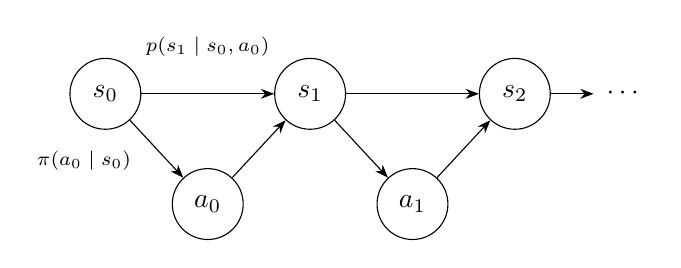
\begin{tikzpicture}[>=Stealth,
  n/.style={circle,draw,minimum size=0.9cm}]
  \node[n](s0)at(0,1.4){$s_0$};\node[n](s1)at(2.6,1.4){$s_1$};\node[n](s2)at(5.2,1.4){$s_2$};
  \node[n](a0)at(1.3,0){$a_0$};\node[n](a1)at(3.9,0){$a_1$};
  \node at (6.6,1.4){$\cdots$};
  \draw[->](s0)--(s1);\draw[->](s1)--(s2);\draw[->](s0)--(a0);\draw[->](a0)--(s1);
  \draw[->](s1)--(a1);\draw[->](a1)--(s2);\draw[->](s2)--(6.2,1.4);
  \node[font=\scriptsize] at (1.3,2.0){$p(s_1\mid s_0,a_0)$};
  \node[font=\scriptsize,anchor=east] at (0.45,0.55){$\pi(a_0\mid s_0)$};
\end{tikzpicture}
\caption{Graphical model of a trajectory (slide 24, redrawn).}
\end{figure}

\begin{intuition}
Each factor is one coin flip: the agent's flip ($\pi$) followed by the world's flip ($p$). Numbers: if $\pi(a_0|s_0)=0.5$, $p(s_1|s_0,a_0)=0.9$ and $\pi(a_1|s_1)=1$, then the probability of the length-2 trajectory $(s_0,a_0,s_1,a_1)$ is $0.5\cdot0.9\cdot1=0.45$.
\end{intuition}

%=====================================================================
\section{State Visitation Probability \slr{25--27}}
%=====================================================================
\subsection{Definition \slr{25}}
What is the probability of visiting $(s,a)$ at time $t$ when following $\pi$ from $s_0$? Marginalise the trajectory probability over everything except the last pair:
\[
  \PP^\pi_t(s,a;s_0)=\sum_{a_0,s_1,a_1,\dots,s_{t-1},a_{t-1}}\PP^\pi(s_0,a_0,\dots,s_t=s,a_t=a).
\]

\begin{intuition}
It answers ``if I run the policy many times, in what fraction of the runs am I in $(s,a)$ at time $t$?'' Plotting it for every state gives a heat map that moves and spreads with $t$.
\end{intuition}

\subsection{Examples \slr{26--27}}
Slide 26 shows, for a policy that goes to the goal in a gridworld with $10\%$ slip, the visitation probability estimated over $2000$ simulations, together with the probability mass in the (absorbing) goal as a function of $t$. Slide 27 shows the same for a \emph{random} policy, on a log scale: the mass at the goal stays essentially $0$.

\begin{figure}[htbp]
\centering
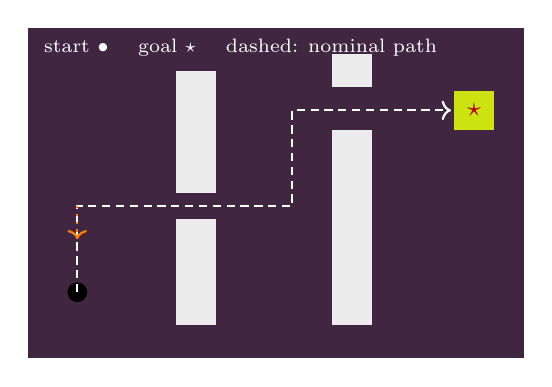
\begin{tikzpicture}[scale=0.42]
  \fill[violet!25!black!85] (0,0) rectangle (15,10);
  \fill[gray!15] (4.5,1) rectangle (5.7,4.2);
  \fill[gray!15] (4.5,5) rectangle (5.7,8.7);
  \fill[gray!15] (9.2,1) rectangle (10.4,6.9);
  \fill[gray!15] (9.2,8.2) rectangle (10.4,9.2);
  \fill[yellow!80!green] (12.9,6.9) rectangle (14.1,8.1);
  \node[red!70!black] at (13.5,7.5) {$\star$};
  \fill[black] (1.5,2) circle (0.3);
  \draw[->,thick,white,dash pattern=on 3pt off 2pt] (1.5,2)--(1.5,4.6)--(8,4.6)--(8,7.5)--(12.8,7.5);
  \draw[->,orange,dotted,thick] (1.5,4.6)--(1.5,3.6);
  \node[white,font=\scriptsize,anchor=west] at (0.2,9.4) {start $\bullet$ \quad goal $\star$ \quad dashed: nominal path};
\end{tikzpicture}
\hfill
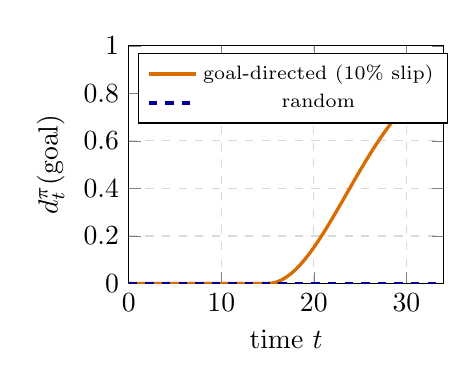
\begin{tikzpicture}
\begin{axis}[width=0.46\linewidth,height=4.6cm,xlabel={time $t$},ylabel={$d^\pi_t(\text{goal})$},
  xmin=0,xmax=34,ymin=0,ymax=1,grid=both,grid style={dashed,gray!30},domain=0:34,samples=69,
  legend style={font=\scriptsize,at={(0.03,0.97)},anchor=north west}]
 \addplot[orange!85!black,very thick]{(x>15)*0.95*(1-exp(-((x-15)/12)^2))};
 \addplot[blue!60!black,very thick,dashed]{0.0005};
 \legend{goal-directed ($10\%$ slip),random}
\end{axis}
\end{tikzpicture}
\caption{Schematic gridworld (left) and shape of the probability mass at the absorbing goal (right) for a goal-directed policy versus a random one. The curve is an original schematic read off slides 26--27, \emph{not} the data of the slide.}
\end{figure}

\begin{figure}[H]
	\centering
	\includegraphics[width=1.0\linewidth]{1790936537236.png}
	\caption{Heat map of $d^\pi_t(s)$ for the goal-directed policy (10\% slip, 2000 simulations) with the ``mass at the goal'' curve.}\label{fig:1790936537236}
\end{figure}

\begin{figure}[H]
	\centering
	\includegraphics[width=1.0\linewidth]{1790936575533.png}
	\caption{Same for the random policy, probability on log scale.}\label{fig:1790936575533}
\end{figure}
\begin{intuition}
Under the goal-directed policy nothing reaches the goal for the first ${\sim}15$ steps (that is the minimum distance), then the mass climbs towards $1$; the missing mass is runs that slipped and are still on the way. The random policy diffuses over the grid so thinly that its goal mass is almost $0$ at every time: the visitation distribution is a fingerprint of the policy's behaviour.
\end{intuition}

%=====================================================================
\section{Another Example MDP \slr{28}}
%=====================================================================
A robotic arm that must move a ball (slide 28):
\begin{itemize}[nosep]
  \item \textbf{state:} robot configuration (joint states) and ball position;
  \item \textbf{action:} torque on arm and finger joints;
  \item \textbf{transition:} stochastic, physics plus noise;
  \item \textbf{policy:} mapping from robot state and ball position to torque;
  \item \textbf{cost:} magnitude of the torque and distance to the goal.
\end{itemize}

\begin{figure}[H]
	\centering
	\includegraphics[width=1.0\linewidth]{1790936625953.png}
	\caption{Photo of a robotic arm manipulating a ball}\label{fig:1790936625953}
\end{figure}
\begin{intuition}
Same five ingredients, a very different world: continuous states and actions, physics instead of a table of probabilities, and a cost made of two competing terms (effort and distance to goal). The abstract tuple $(\cS,\cA,p,r)$ covers both the toy table above and a robot.
\end{intuition}

%=====================================================================
\section{Infinite Horizon Discounted Setting \slr{29}}
%=====================================================================
So far the MDP is $(\cS,\cA,p,r)$. We now add a discount factor $\gamma$ to reason about the long-term effects of a policy, with $\gamma$ in $[0,1]$ on the slide: $\gamma=0$ means ``I only care about immediate rewards'', while $\gamma=1$ means immediate and future rewards are equally important. The slide leaves ``How so?'' as a question; it is answered in ``Back to Discount Factor'' below, where we see that $\gamma=1$ is a bad idea for infinite tasks and the formal definition (Definition~\ref{def:mdp}) takes $\gamma<1$.

\begin{intuition}
$\gamma$ is a patience dial. At $\gamma=0.5$ a reward two steps away is worth $0.25$ of the same reward now; at $\gamma=0.99$ it is worth $0.98$.
\end{intuition}

%=====================================================================
\section{Value Function \slr{30--31}}
%=====================================================================
We estimate the \emph{goodness} of states and actions by their value, which is also a measure to compare policies. The state-value function of a policy $\pi$ is the expected discounted return from $s$ (slide 30):
\begin{align*}
  V^\pi(s_t)&=\E\!\left[r_t+\gamma r_{t+1}+\gamma^2r_{t+2}+\cdots\mid s_t\right]\\
  &=\E\!\left[\sum_{h=0}^{\infty}\gamma^hr_{t+h}\;\Big|\;s_t=s,\ a_h=\pi(s_h),\ s_{h+1}\sim p(\cdot\mid s_h,a_h)\right].
\end{align*}
Slide 31 adds the action-value function, where the first action is fixed and then $\pi$ is followed:
\begin{align*}
  Q^\pi(s_t,a_t)=\E\!\Big[\sum_{h=0}^{\infty}\gamma^hr_{t+h}\;\Big|\;&(s_t,a_t)=(s,a),\\
  &a_h=\pi(s_h),\ s_{h+1}\sim p(\cdot\mid s_h,a_h)\Big].
\end{align*}

\begin{intuition}
$V^\pi(s)$: ``how good is it to \emph{be} in $s$ if I then follow $\pi$?'' $Q^\pi(s,a)$: ``how good is it to take $a$ \emph{now} in $s$ and then follow $\pi$?'' The difference between the two is one free first decision. Comparing $Q^\pi(s,a)$ across $a$ is how an agent decides which action is better than the policy's current choice.
\end{intuition}

%=====================================================================
\section{Back to Discount Factor \slr{32}}
%=====================================================================
Setting $\gamma=1$ for infinite tasks is a bad idea. The quantity $\sum_{h=0}^\infty\gamma^h$ is a geometric series, equal to $1/(1-\gamma)$ for $\gamma\in[0,1)$, so the value of $\gamma$ approximately determines how many steps ahead we are looking: e.g.\ $\gamma=0.99$ corresponds to ${\sim}100$ time steps.

\begin{lemma}[Values are finite, and how finite]\label{lem:bound}
For every policy and every state, $0\le V^\pi(s)\le\dfrac{\Rmax}{1-\gamma}$.
\end{lemma}
\begin{proof}
Rewards lie in $[0,\Rmax]$, so $0\le\sum_h\gamma^hr_h\le\Rmax\sum_{h\ge0}\gamma^h=\Rmax/(1-\gamma)$, the geometric series converging because $\gamma<1$. Expectations preserve the bounds.
\end{proof}

\begin{figure}[htbp]
\centering
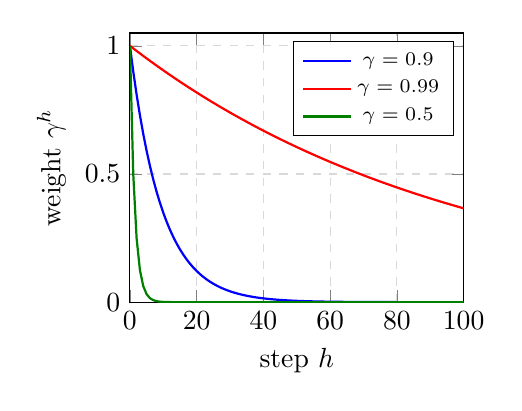
\begin{tikzpicture}
\begin{axis}[width=0.48\linewidth,height=5cm,xlabel={step $h$},ylabel={weight $\gamma^h$},xmin=0,xmax=100,ymin=0,ymax=1.05,
  legend style={font=\scriptsize,at={(0.97,0.97)},anchor=north east},domain=0:100,samples=101,grid=both,grid style={dashed,gray!30}]
 \addplot[blue,thick]{0.9^x};
 \addplot[red,thick]{0.99^x};
 \addplot[green!50!black,thick]{0.5^x};
 \legend{$\gamma=0.9$,$\gamma=0.99$,$\gamma=0.5$}
\end{axis}
\end{tikzpicture}
\hfill
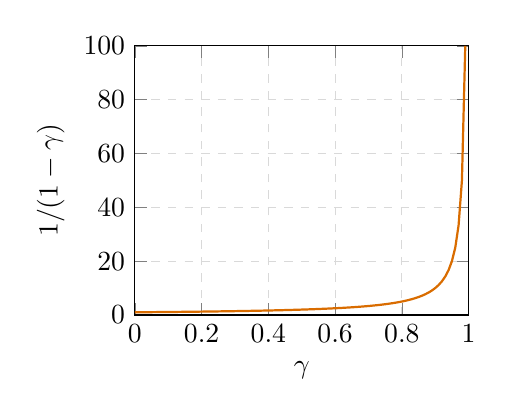
\begin{tikzpicture}
\begin{axis}[width=0.48\linewidth,height=5cm,xlabel={$\gamma$},ylabel={$1/(1-\gamma)$},xmin=0,xmax=1,ymin=0,ymax=100,
  domain=0:0.99,samples=100,grid=both,grid style={dashed,gray!30}]
 \addplot[orange!85!black,thick]{1/(1-x)};
\end{axis}
\end{tikzpicture}
\caption{Left: discount weights $\gamma^h$. Right: the effective horizon $1/(1-\gamma)$ diverges as $\gamma\to1$ (original figures for slide 32).}
\end{figure}

\begin{intuition}
With $\gamma=0.99$ the weight $\gamma^{h}$ falls to $\gamma^{100}\approx0.37\approx1/e$ after about $100$ steps; with $\gamma=0.9$ the same happens after about $10$ steps. If rewards are at most $\Rmax=1$, the value can never exceed $1/(1-0.99)=100$; at $\gamma=1$ the bound is infinite and the sum of rewards of an endless task need not exist at all. The discount is what makes ``the value of a state'' a well-defined finite number.
\end{intuition}

%=====================================================================
\section{Bellman Equation \slr{33--36}}
%=====================================================================
The value of a state is expanded in terms of the current reward and the value of the next states according to the policy (slide 33): for a deterministic $\pi$,
\[
  V^\pi(s_t)=\E_\pi\!\left[r_t+\gamma r_{t+1}+\gamma^2r_{t+2}+\cdots\mid s_t\right]=r_t+\gamma\,\E_{s'\sim p(\cdot\mid s_t,\pi(s_t))}\!\left[V^\pi(s')\right],
\]
and likewise for $Q$ (slides 34--36):
\[
  Q^\pi(s_t,a_t)=r_t+\gamma\,\E_{s'\sim p(\cdot\mid s_t,a_t)}\!\left[V^\pi(s')\right].
\]
In the first equation $r$ is a function of $s$ and $\pi(s)$; in the second, of $s$ and $a$. As a result $V^\pi(s)=Q^\pi(s,\pi(s))$ (slide 36).

\begin{theorem}[Bellman expectation equations]\label{thm:bellexp}
For every policy $\pi$ and all $s,a$:
\begin{align*}
 V^\pi(s)&=\E_{a\sim\pi(\cdot\mid s)}\Big[r(s,a)+\gamma\,\E_{s'\sim p(\cdot\mid s,a)}\big[V^\pi(s')\big]\Big],\\
 Q^\pi(s,a)&=r(s,a)+\gamma\,\E_{s'\sim p(\cdot\mid s,a)}\big[V^\pi(s')\big],\\
 V^\pi(s)&=\E_{a\sim\pi(\cdot\mid s)}\big[Q^\pi(s,a)\big].
\end{align*}
For a deterministic policy the first reads $V^\pi(s)=r(s,\pi(s))+\gamma\E_{s'\sim p(\cdot\mid s,\pi(s))}[V^\pi(s')]$ and the last $V^\pi(s)=Q^\pi(s,\pi(s))$.
\end{theorem}
\begin{proof}
Split the return after the first step using $G_0=r(s_0,a_0)+\gamma G_1$:
$V^\pi(s)=\E^\pi[G_0\mid s_0=s]=\E^\pi[r(s_0,a_0)\mid s_0=s]+\gamma\E^\pi[G_1\mid s_0=s]$.
Condition the second term on $(a_0,s_1)$ and use the tower rule. By Definition~\ref{def:markov} and the fact that $\pi$ depends only on the current state, the conditional distribution of the trajectory from $s_1$ onwards given $(s_0,a_0,s_1)$ is the same as that of a trajectory started at $s_1$; hence $\E^\pi[G_1\mid s_0=s,a_0=a,s_1=s']=V^\pi(s')$. Averaging over $s'\sim p(\cdot\mid s,a)$ and then over $a\sim\pi(\cdot\mid s)$ gives the first identity; the argument for $Q^\pi$ is the same with $a_0$ fixed.
\end{proof}

\begin{figure}[htbp]
\centering
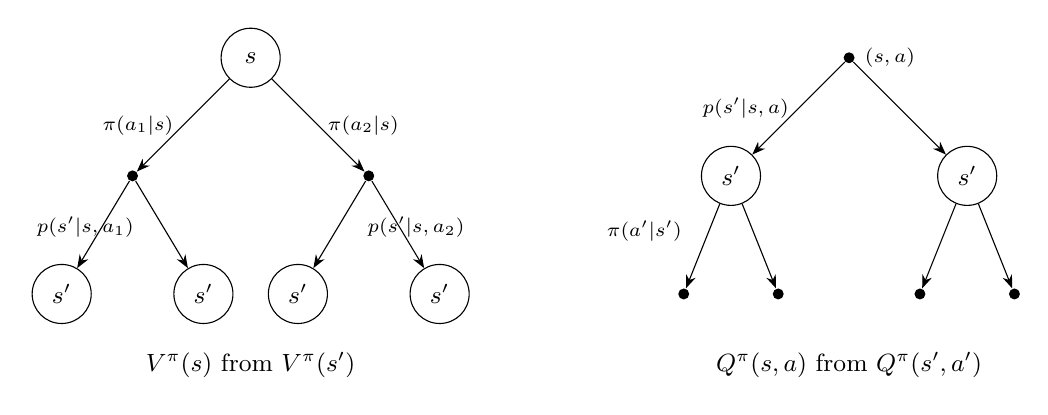
\begin{tikzpicture}[>=Stealth,
  s/.style={circle,draw,minimum size=0.75cm,font=\small},
  a/.style={circle,fill=black,inner sep=1.4pt}]
  % V backup
  \begin{scope}
   \node[s](v) at (0,3){$s$};
   \node[a](a1) at (-1.5,1.5){};\node[a](a2) at (1.5,1.5){};
   \draw[->](v)--(a1) node[pos=0.5,left,font=\scriptsize]{$\pi(a_1|s)$};
   \draw[->](v)--(a2) node[pos=0.5,right,font=\scriptsize]{$\pi(a_2|s)$};
   \node[s](na) at (-2.4,0){$s'$};\node[s](nb) at (-0.6,0){$s'$};
   \node[s](nc) at (0.6,0){$s'$};\node[s](nd) at (2.4,0){$s'$};
   \draw[->](a1)--(na);\draw[->](a1)--(nb);\draw[->](a2)--(nc);\draw[->](a2)--(nd);
   \node[font=\scriptsize] at (-2.1,0.85){$p(s'|s,a_1)$};
   \node[font=\scriptsize] at (2.1,0.85){$p(s'|s,a_2)$};
   \node[font=\small] at (0,-0.9){$V^\pi(s)$ from $V^\pi(s')$};
  \end{scope}
  % Q backup
  \begin{scope}[xshift=7.6cm]
   \node[a,label=right:{\scriptsize $(s,a)$}](q) at (0,3){};
   \node[s](ml) at (-1.5,1.5){$s'$};\node[s](mr) at (1.5,1.5){$s'$};
   \draw[->](q)--(ml) node[pos=0.5,left,font=\scriptsize]{$p(s'|s,a)$};\draw[->](q)--(mr);
   \node[a](b1) at (-2.1,0){};\node[a](b2) at (-0.9,0){};\node[a](b3) at (0.9,0){};\node[a](b4) at (2.1,0){};
   \draw[->](ml)--(b1);\draw[->](ml)--(b2);\draw[->](mr)--(b3);\draw[->](mr)--(b4);
   \node[font=\scriptsize] at (-2.6,0.8){$\pi(a'|s')$};
   \node[font=\small] at (0,-0.9){$Q^\pi(s,a)$ from $Q^\pi(s',a')$};
  \end{scope}
\end{tikzpicture}
\caption{Backup diagrams for the Bellman expectation equations (original figure for slides 33--36).}
\end{figure}

\begin{intuition}
The equation says: \emph{value now = reward now + discounted value of where I land}. It turns an infinite sum into a one-step consistency condition. Example (deterministic): if $r(s,\pi(s))=1$, $\gamma=0.9$ and the next state always has value $V^\pi(s')=10$, then $V^\pi(s)=1+0.9\cdot10=10$. The two lines of the theorem differ only in what is averaged: $V$ averages over my action choice (policy), $Q$ has the first action already fixed and averages only over the environment's randomness.
\end{intuition}

%=====================================================================
\section{Discounted State-Action Distribution \slr{37--38}}
%=====================================================================
\begin{definition}[Discounted state-action distribution]\label{def:dsa}
\[
  d^\pi_{s_0}(s,a)=(1-\gamma)\sum_{h=0}^{\infty}\gamma^h\,\PP^\pi_h(s,a;s_0).
\]
For an initial distribution $\mu$ write $d^\pi_\mu(s,a)=\E_{s_0\sim\mu}[d^\pi_{s_0}(s,a)]$.
\end{definition}

\begin{lemma}[It is a distribution, and that is the point of the $(1-\gamma)$]\label{lem:dist}
$d^\pi_{s_0}$ is a probability distribution over $\cS\times\cA$.
\end{lemma}
\begin{proof}
Non-negativity is clear. Summing over $(s,a)$ and exchanging the (absolutely convergent) sums,
$\sum_{s,a}d^\pi_{s_0}(s,a)=(1-\gamma)\sum_h\gamma^h\sum_{s,a}\PP^\pi_h(s,a;s_0)=(1-\gamma)\sum_h\gamma^h=1$, since $\PP^\pi_h(\cdot;s_0)$ is a distribution for each $h$.
\end{proof}
This matches the slide's remark: ``this gives us a probability distribution (remember $\sum_h\gamma^h=1/(1-\gamma)$)''. The companion identity expressing discounted sums as expectations under $d^\pi_{s_0}$ is not on the slides and is given in Appendix~\ref{app:identity}.

\begin{intuition}
Take the visitation probabilities of the previous section, weight time step $h$ by $\gamma^h$ and sum them: this is ``how much total (discounted) time I spend in $(s,a)$''. Without the factor $(1-\gamma)$ the total mass would be $1/(1-\gamma)$ (e.g.\ $100$ for $\gamma=0.99$); multiplying by $(1-\gamma)$ rescales it to $1$ so it can be used as a genuine probability distribution. Early time steps get most of the weight, which is the same patience dial as before.
\end{intuition}

%=====================================================================
\section{Optimal Policy \slr{39--40}}
%=====================================================================
\begin{definition}[Optimal value and optimal policy]\label{def:opt}
$V^\star(s)=\sup_\pi V^\pi(s)$ and $Q^\star(s,a)=\sup_\pi Q^\pi(s,a)$. A policy $\pi^\star$ is optimal if $V^{\pi^\star}(s)=V^\star(s)$ for every $s$.
\end{definition}

Slides 39--40 state that for infinite-horizon MDPs there \emph{always} exists a deterministic policy $\pi^\star$ such that
\[
  V^{\pi^\star}(s)\ge V^\pi(s)\qquad\forall s,\pi,
\]
i.e.\ $\pi^\star$ dominates all other policies in each state; it returns optimal actions $a^\star$, and $V^{\pi^\star}=V^\star$, $Q^{\pi^\star}=Q^\star$. The existence statement is proved constructively by Theorem~\ref{thm:greedy} below.

\begin{intuition}
It is far from obvious that one policy can be best \emph{in all states simultaneously}; in many optimisation problems the best choice for one objective hurts another. Here it is true, and it is also true that we never need randomness: a table of ``best action in each state'' suffices. This is what makes the search for optimal behaviour tractable.
\end{intuition}

%=====================================================================
\section{Bellman Optimality \slr{41--42}}
%=====================================================================
\begin{theorem}[Bellman optimality equation]\label{thm:bellopt}
\begin{align*}
 V^\star(s)&=\max_a\Big[r(s,a)+\gamma\,\E_{s'\sim p(\cdot\mid s,a)}V^\star(s')\Big],\\
 Q^\star(s,a)&=r(s,a)+\gamma\,\E_{s'\sim p(\cdot\mid s,a)}\Big[\max_{a'}Q^\star(s',a')\Big].
\end{align*}
\end{theorem}
On slide 42 the bracket $r(s,a)+\gamma\E_{s'}V^\star(s')$ is annotated as $Q^\star(s,a)$, so that $V^\star(s)=\max_aQ^\star(s,a)$.

\begin{intuition}
The Bellman \emph{expectation} equation averages over the policy's action; the Bellman \emph{optimality} equation replaces that average by a $\max$: the optimal agent simply takes the best action. All the difficulty of looking arbitrarily far into the future is hidden in $V^\star(s')$: if I knew the optimal value of every neighbour, choosing the best action would be a one-step problem.
\end{intuition}

%=====================================================================
\section{Bellman Optimality Example \slr{43--45}}
%=====================================================================
Assume we know $V^\star$ at $s'$ and $s''$, the two successors of $s$ reached by actions $a'$ and $a''$ (slide 43). Try $a'$, get $r(s,a')$ and compute $Q^\star(s,a')=r(s,a')+\gamma V^\star(s')$; try $a''$ and compute $Q^\star(s,a'')=r(s,a'')+\gamma V^\star(s'')$ (slide 44). Then (slide 45)
\[
  V^\star(s)=\max_{a',a''}\{Q^\star(s,a'),\,Q^\star(s,a'')\}.
\]

\begin{figure}[htbp]
\centering
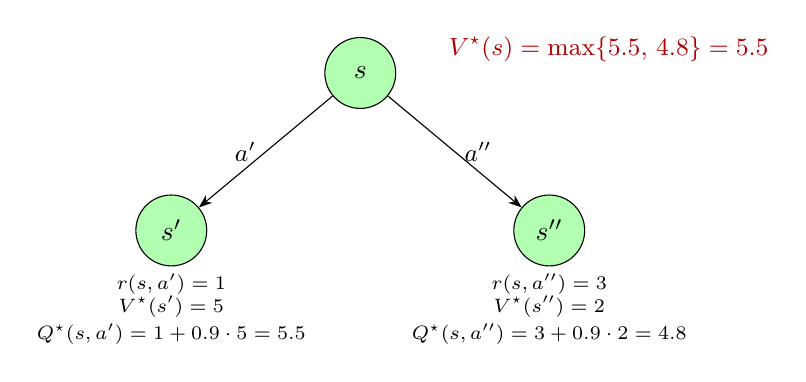
\begin{tikzpicture}[>=Stealth,
  n/.style={circle,draw,fill=green!30,minimum size=0.9cm}]
  \node[n](s) at (0,2){$s$};
  \node[n](s1) at (-2.4,0){$s'$};
  \node[n](s2) at (2.4,0){$s''$};
  \draw[->](s)--(s1) node[midway,left,font=\small]{$a'$};
  \draw[->](s)--(s2) node[midway,right,font=\small]{$a''$};
  \node[font=\scriptsize,align=center] at (-2.4,-1.0){$r(s,a')=1$\\$V^\star(s')=5$\\[2pt]$Q^\star(s,a')=1+0.9\cdot5=5.5$};
  \node[font=\scriptsize,align=center] at (2.4,-1.0){$r(s,a'')=3$\\$V^\star(s'')=2$\\[2pt]$Q^\star(s,a'')=3+0.9\cdot2=4.8$};
  \node[red!70!black,font=\small,anchor=west] at (1.0,2.3){$V^\star(s)=\max\{5.5,\,4.8\}=5.5$};
\end{tikzpicture}
\caption{The one-step lookahead of slides 43--45 with illustrative numbers ($\gamma=0.9$; the numbers are mine, not the slide's).}
\end{figure}

\begin{intuition}
With the numbers above the action with the \emph{larger immediate reward} ($a''$, reward $3$) is \emph{not} the best: $a'$ leads to a state worth $5$, and $1+4.5>3+1.8$. This is the one-step trick that everything else in the course rests on: evaluate each action as ``reward + discounted value of where it leads'' and take the best.
\end{intuition}

%=====================================================================
\section{Bellman Optimality (Theorem 1) \slr{46--49}}
%=====================================================================
\begin{theorem}[Theorem 1 --- greedy with respect to $Q^\star$ is optimal]\label{thm:greedy}
Let $\hat\pi(s)\in\argmax_aQ^\star(s,a)$. Then $V^{\hat\pi}=V^\star$, and therefore $\pi^\star=\hat\pi$ is an optimal policy.
\end{theorem}

\subsection*{Proof as shown on the slides (slides 46--48)}
Starting from $V^\star(s)=\max_a[r(s,a)+\gamma\E_{s'}V^\star(s')]$ and unrolling the equation along $\hat\pi$:
\begin{align*}
V^\star(s)&=r(s,\pi^\star(s))+\gamma\E_{s'}V^\star(s')\\
&\le\max_a\Big[r(s,a)+\gamma\E_{s'}V^\star(s')\Big]=r(s,\hat\pi(s))+\gamma\E_{s'}V^\star(s')\\
&\le r(s,\hat\pi(s))+\gamma\E_{s'\sim p(\cdot|s,\hat\pi(s))}\Big[r(s',\hat\pi(s'))+\gamma\E_{s''}V^\star(s'')\Big]\\
&\le\cdots\le\E\Big[r(s,\hat\pi(s))+\gamma r(s',\hat\pi(s'))+\cdots\Big]=V^{\hat\pi}(s),
\end{align*}
so $V^{\hat\pi}\ge V^\star$ (the leftover term $\gamma^k\E V^\star(s_k)\to0$ since $V^\star$ is bounded, Lemma~\ref{lem:bound}); and $V^\star\ge V^{\hat\pi}$ holds by definition of $V^\star$ as a supremum. Hence $V^{\hat\pi}=V^\star$ and, by slide 49, $\pi^\star=\argmax_aQ^\star(s,a)$ is an optimal policy.

\subsection*{Proof in the companion text (fixed-point argument)}
\begin{proof}
By Theorem~\ref{thm:bellopt}, $V^\star=\mathcal BV^\star$ and $Q^\star(s,a)=r(s,a)+\gamma\E_{s'}[V^\star(s')]$ (the operators $\mathcal B,\mathcal B^{\hat\pi}$ are recalled in Appendix~\ref{app:ops}). Since $\hat\pi(s)$ maximises $Q^\star(s,\cdot)$,
\[
(\mathcal BV^\star)(s)=\max_aQ^\star(s,a)=Q^\star\big(s,\hat\pi(s)\big)=r\big(s,\hat\pi(s)\big)+\gamma\E_{s'\sim p(\cdot|s,\hat\pi(s))}\big[V^\star(s')\big]=(\mathcal B^{\hat\pi}V^\star)(s),
\]
so $V^\star$ is a fixed point of $\mathcal B^{\hat\pi}$. By Theorem~\ref{thm:bellexp} so is $V^{\hat\pi}$, and both are bounded by Lemma~\ref{lem:bound}.

A bounded fixed point of $\mathcal B^{\hat\pi}$ is unique. If $u$ and $v$ are two, then for every $s$
\[
|u(s)-v(s)|=\gamma\Big|\E_{s'}\big[u(s')-v(s')\big]\Big|\le\gamma\|u-v\|_\infty,
\]
because the rewards cancel, so $\|u-v\|_\infty\le\gamma\|u-v\|_\infty$. The norm is finite and $\gamma<1$, hence $u=v$. Therefore $V^{\hat\pi}=V^\star$, and $\hat\pi$ attains the supremum of Definition~\ref{def:opt} at every state.
\end{proof}

\begin{intuition}
Theorem~1 is the license to \emph{act}: once someone hands me $Q^\star$, I do not need to plan any more; the single-step rule ``pick the action with the largest $Q^\star(s,\cdot)$'' is already globally optimal. The slide proof says it as a sandwich: following $\hat\pi$ can't be better than optimal ($V^{\hat\pi}\le V^\star$), and by unrolling the optimality equation it can't be worse either ($V^{\hat\pi}\ge V^\star$). The book proof says the same thing differently: $V^\star$ and $V^{\hat\pi}$ solve the same one-policy equation, and that equation has only one bounded solution because each application shrinks distances by $\gamma<1$.
\end{intuition}

%=====================================================================
\section{Bellman Optimality (Theorem 2) \slr{50--55}}
%=====================================================================
\begin{theorem}[Theorem 2 --- the optimality equation has one solution]\label{thm:unique}
If $V:\cS\to\mathbb R$ satisfies $V(s)=\max_a\big[r(s,a)+\gamma\E_{s'\sim p(\cdot|s,a)}V(s')\big]$ for every $s$, then $V=V^\star$.
\end{theorem}
The slides (51--53) ask us to check that $\|V-V^\star\|_\infty=0$ and then unroll the difference.
\begin{proof}
Both $V$ and $V^\star$ satisfy the same equation, so for every $s$,
\begin{align*}
|V(s)-V^\star(s)|&=\Big|\max_a\big[r(s,a)+\gamma\E_{s'}V(s')\big]-\max_a\big[r(s,a)+\gamma\E_{s'}V^\star(s')\big]\Big|\\
&\le\max_a\Big|\big[r(s,a)+\gamma\E_{s'}V(s')\big]-\big[r(s,a)+\gamma\E_{s'}V^\star(s')\big]\Big|\\
&=\max_a\gamma\Big|\E_{s'\sim p(\cdot|s,a)}\big[V(s')-V^\star(s')\big]\Big|\\
&\le\gamma\max_a\E_{s'\sim p(\cdot|s,a)}\big|V(s')-V^\star(s')\big|.
\end{align*}
The first inequality is $|\max_af(a)-\max_ag(a)|\le\max_a|f(a)-g(a)|$; the last is Jensen. Applying the same bound to $|V(s')-V^\star(s')|$ and iterating $k$ times,
\[
|V(s)-V^\star(s)|\le\gamma^k\max_{a_0,\dots,a_{k-1}}\E_{s_k}\big|V(s_k)-V^\star(s_k)\big|\le\gamma^k\|V-V^\star\|_\infty,
\]
and since $\gamma<1$ and $\|V-V^\star\|_\infty$ is finite, the right-hand side tends to $0$. Hence $|V(s)-V^\star(s)|=0$ for every $s$.
\end{proof}

Slide 54 illustrates the shrinking bound $\gamma^h\|V-V^\star\|_\infty$ as the number of future steps $h$ grows (its example uses $\gamma=0.92$ and a baseline $\|V-V^\star\|_\infty=1$).

\begin{figure}[htbp]
\centering
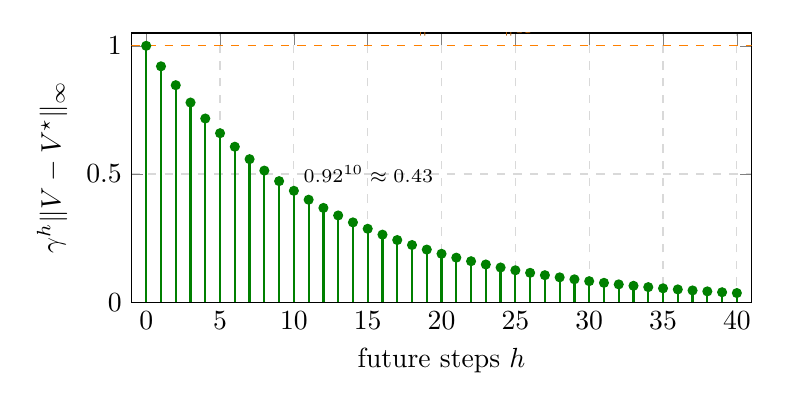
\begin{tikzpicture}
\begin{axis}[width=0.78\linewidth,height=5cm,xlabel={future steps $h$},ylabel={$\gamma^h\|V-V^\star\|_\infty$},
  xmin=-1,xmax=41,ymin=0,ymax=1.05,grid=both,grid style={dashed,gray!30}]
 \addplot[ycomb,green!50!black,thick,mark=*,mark size=1.4pt,domain=0:40,samples=41]{0.92^x};
 \draw[dashed,orange] (axis cs:-1,1)--(axis cs:41,1);
 \node[orange!70!black,font=\scriptsize,anchor=south west] at (axis cs:12,1.0){baseline $\|V-V^\star\|_\infty=1$};
 \node[font=\scriptsize,anchor=west] at (axis cs:10,0.5){$0.92^{10}\approx0.43$};
\end{axis}
\end{tikzpicture}
\caption{The bound $\gamma^h\|V-V^\star\|_\infty$ for $\gamma=0.92$, redrawn from the idea of slide 54 (values computed here).}
\end{figure}

\begin{figure}[H]
	\centering
	\includegraphics[width=1.0\linewidth]{1790936669032.png}
	\caption{Shrinking bound}\label{fig:1790936669032}
\end{figure}
\begin{intuition}
Imagine a ``fake'' value function $V$ that satisfies the optimality equation and is not $V^\star$. Each time we expand the equation one step, the gap can be at most $\gamma$ times what it was; after $k$ steps it is at most $\gamma^k$ times the original gap, which melts away (with $\gamma=0.92$, $0.92^{56}<0.01$). The only way for the gap to survive all expansions is to be $0$. Slide 55 states the consequence: \emph{we can focus on one step at a time}, leaving the rest of the problem to $V(s')$, and any $V$ satisfying that one-step formula is in fact $V^\star$.
\end{intuition}

%=====================================================================
\section{Summary}
%=====================================================================
\begin{center}
\small
\renewcommand{\arraystretch}{1.35}
\begin{tabular}{@{}>{\raggedright\arraybackslash}p{2.9cm}>{\raggedright\arraybackslash}p{6.3cm}>{\raggedright\arraybackslash}p{4.5cm}c@{}}
\toprule
\textbf{Object / result} & \textbf{Formula} & \textbf{What it tells us} & \textbf{Slides}\\
\midrule
Markov state & $p(s_{t+1}|s_t,a_t)=p(s_{t+1}|h_t,a_t)$ & the present summarises the past & 15--17\\
MDP & $(\cS,\cA,p,r,\gamma)$ & sequential decisions with consequences & 18--29\\
$V^\pi$, $Q^\pi$ & $\E[\sum_h\gamma^hr_{t+h}\mid\cdot]$ & how good a state / action is under $\pi$ & 30--31\\
Finite values & $0\le V^\pi\le\Rmax/(1-\gamma)$ & why $\gamma<1$ & 32\\
Bellman expectation & $V^\pi(s)=\E_a[r+\gamma\E_{s'}V^\pi(s')]$ & one-step consistency of a given policy & 33--36\\
$d^\pi_{s_0}$ & $(1-\gamma)\sum_h\gamma^h\PP^\pi_h$ & discounted occupancy, a true distribution & 37--38\\
Optimal $V^\star,Q^\star$ & $\sup_\pi V^\pi$, $\sup_\pi Q^\pi$ & a deterministic policy dominates all others & 39--40\\
Bellman optimality & $V^\star(s)=\max_a[r+\gamma\E_{s'}V^\star(s')]$ & one-step lookahead with a $\max$ & 41--45\\
Theorem 1 & $\hat\pi\in\argmax_aQ^\star\Rightarrow V^{\hat\pi}=V^\star$ & greedy w.r.t.\ $Q^\star$ is optimal & 46--49\\
Theorem 2 & $V=\max_a[r+\gamma\E V]\Rightarrow V=V^\star$ & $V^\star$ is the unique solution & 50--55\\
\bottomrule
\end{tabular}
\end{center}

\begin{figure}[htbp]
\centering
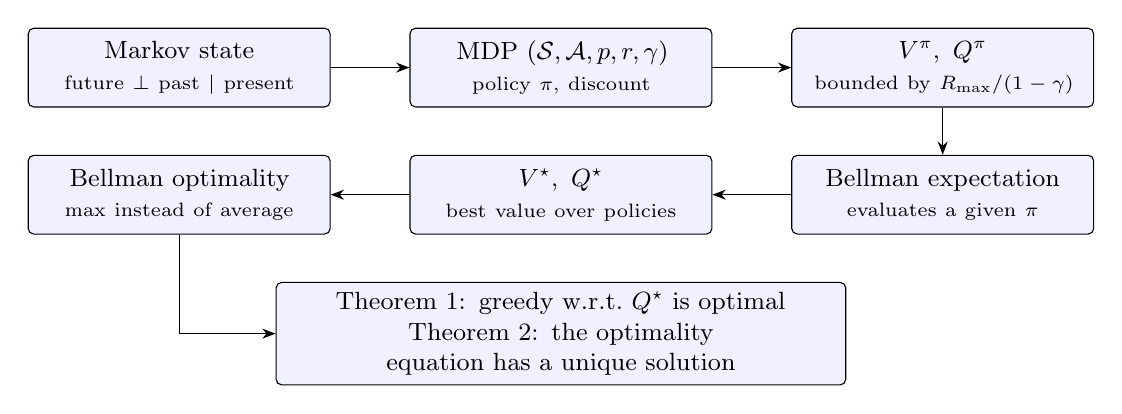
\begin{tikzpicture}[>=Stealth,node distance=6mm and 10mm,
  b/.style={draw,rounded corners=2pt,fill=blue!6,align=center,minimum height=1.0cm,text width=3.6cm,font=\small}]
  \node[b](m){Markov state\\{\scriptsize future $\perp$ past $\mid$ present}};
  \node[b,right=of m](d){MDP $(\cS,\cA,p,r,\gamma)$\\{\scriptsize policy $\pi$, discount}};
  \node[b,right=of d](v){$V^\pi,\ Q^\pi$\\{\scriptsize bounded by $\Rmax/(1-\gamma)$}};
  \node[b,below=of v](be){Bellman expectation\\{\scriptsize evaluates a given $\pi$}};
  \node[b,left=of be](vs){$V^\star,\ Q^\star$\\{\scriptsize best value over policies}};
  \node[b,left=of vs](bo){Bellman optimality\\{\scriptsize $\max$ instead of average}};
  \node[b,below=of vs,text width=7cm](th){Theorem 1: greedy w.r.t.\ $Q^\star$ is optimal\\Theorem 2: the optimality equation has a unique solution};
  \draw[->](m)--(d);\draw[->](d)--(v);\draw[->](v)--(be);\draw[->](be)--(vs);\draw[->](vs)--(bo);\draw[->](bo)|-(th);
\end{tikzpicture}
\caption{Roadmap of the lecture: from the Markov assumption to optimal policies.}
\end{figure}

\subsection*{Key take-aways}
\begin{itemize}
  \item An MDP is a contextual bandit whose next context depends on the action taken; the Markov property means the current state is all the agent needs to know.
  \item The discount factor $\gamma<1$ keeps the value finite, with $0\le V^\pi\le\Rmax/(1-\gamma)$, and $1/(1-\gamma)$ is the effective horizon ($\gamma=0.99\Rightarrow{\sim}100$ steps).
  \item Bellman equations turn an infinite-horizon sum into a one-step relation: value now $=$ reward $+$ discounted value of the next state (average for a policy, $\max$ for optimality).
  \item Theorem 1: acting greedily with respect to $Q^\star$ is optimal, so a deterministic stationary policy always suffices.
  \item Theorem 2: $V^\star$ is the \emph{only} solution of the Bellman optimality equation, thanks to the $\gamma$-contraction; any $V$ that satisfies the one-step formula is $V^\star$.
\end{itemize}

%=====================================================================
\appendix
\section{Appendix: supplementary material (in the companion PDF, not on the slides)}
%=====================================================================
The following results appear in the companion PDF but have no corresponding slide; they are \emph{not} part of the slide flow above.

\subsection{Discounted sums as expectations under \texorpdfstring{$d^\pi_{s_0}$}{d}}\label{app:identity}
\begin{lemma}[Second part of Lemma 5 of the PDF]
For every bounded $f$,
\[
  \E^\pi\!\left[\sum_{h=0}^\infty\gamma^hf(s_h,a_h)\;\Big|\;s_0\right]=\frac1{1-\gamma}\,\E_{(s,a)\sim d^\pi_{s_0}}\big[f(s,a)\big].
\]
\end{lemma}
\begin{proof}
It is the same exchange of (absolutely convergent) sums used in the proof of Lemma~\ref{lem:dist}, applied to $f$: $\E^\pi[\sum_h\gamma^hf(s_h,a_h)\mid s_0]=\sum_h\gamma^h\sum_{s,a}\PP^\pi_h(s,a;s_0)f(s,a)=\frac1{1-\gamma}\sum_{s,a}d^\pi_{s_0}(s,a)f(s,a)$.
\end{proof}
\begin{intuition}
Choosing $f=r$ gives $V^\pi(s_0)=\frac1{1-\gamma}\E_{(s,a)\sim d^\pi_{s_0}}[r(s,a)]$: the value is the average reward under the discounted occupancy, scaled by the effective horizon $1/(1-\gamma)$. For $\gamma=0.9$, if the average reward under $d^\pi$ is $0.5$, the value is $0.5/0.1=5$.
\end{intuition}

\subsection{Bellman operators (notation used in the PDF's proofs)}\label{app:ops}
The proof of Theorem~\ref{thm:greedy} in the companion text uses two operators acting on bounded functions $V:\cS\to\mathbb R$:
\begin{align*}
  (\mathcal BV)(s)&=\max_a\Big[r(s,a)+\gamma\E_{s'\sim p(\cdot|s,a)}V(s')\Big],\\
  (\mathcal B^{\pi}V)(s)&=r(s,\pi(s))+\gamma\E_{s'\sim p(\cdot|s,\pi(s))}V(s')\quad(\pi\text{ deterministic}).
\end{align*}
With this notation Theorem~\ref{thm:bellopt} reads $V^\star=\mathcal BV^\star$, Theorem~\ref{thm:bellexp} reads $V^\pi=\mathcal B^\pi V^\pi$, and Theorem~\ref{thm:unique} says that $\mathcal B$ has a unique fixed point. The slides never name these operators.

\newpage

% ======================================================================
% Lecture 3
% ======================================================================
\part{Lecture 3}

\begin{abstract}\noindent
This lecture answers the question left open by the MDP lectures: \emph{how do we actually compute} $V^\pi$ and, above all, the optimal policy $\pi^*$?
We first compute $V^\pi$ exactly (a linear system) and iteratively (a fixed-point iteration), introduce \emph{contraction mappings} as the tool that makes iteration converge, show that both Bellman backups are $\gamma$-contractions, and conclude with \textbf{value iteration}, its convergence rate, the quality of the greedy policy it returns, and the number of iterations needed for an $\epsilon$-optimal policy.
\end{abstract}

\subsection*{How these notes are organised}
\begin{itemize}
  \item \textbf{Sections follow the slide deck}, with the slide range in italics next to each title. Formal material from the companion note is merged where the slides introduce the topic.
  \item \textbf{Numbering.} Definitions, theorems and corollaries \emph{1--8} and algorithms \emph{A, B} keep the numbering of the companion note, so that its self-check list and proof videos map directly (see Appendix~\ref{app:selfcheck}). Items numbered \emph{S, L, E, F} are not in the companion note: \emph{S}/\emph{L} = propositions/lemmas derived on the slides (or needed for completeness), \emph{E} = worked examples, \emph{F} = facts recalled from the previous lecture (L03).
  \item \textbf{Coloured boxes.} Definitions (green), theorems/corollaries (red), propositions/lemmas (orange), examples (teal), algorithms (violet), recalled facts (grey), and blue \emph{Intuition} boxes that explain the ``why'' in plain words.
  \item \textbf{Running example.} A tiny two-state, two-action MDP (Example~\ref{ex:toy}) is used for all worked numbers and for the data-driven plots.
  \item \textbf{Supplementary material} not covered on the slides (the existence/rate part of Banach's theorem) is in Appendix~\ref{app:banach}, clearly labelled.
\end{itemize}
Throughout, rewards lie in $[0,1]$ (so $R_{\max}=1$), $\gamma\in[0,1)$, $\norm{\cdot}$ is the sup-norm, and $\ln$ is the natural logarithm (the slides write $\log$ for it).


\newpage
%=====================================================================
\section{Recap: Sequential Decision Making and MDPs \slides{2--12}}
%=====================================================================
This block repeats what the previous lecture (L03) established. Everything later is built on it, and three of the results are quoted from L03 without proof (Facts F1--F4 below).

\subsection{Sequential Decision Making and the MDP \slides{3--4}}
The agent interacts with its environment at discrete timesteps: at each step it receives an observation $o_t$ and a reward $r_t$ from the environment and answers with an action $a_t$ (\figref{fig:loop}). The \emph{state} is a function of the history, $s_t=f(h_t)$, and is typically hidden or unknown.

A \textbf{Markov Decision Process} is sequential decision making under the Markov assumption: the transition dynamics are Markovian, the state is fully observable, and the dynamics are (in general) stochastic, $p(s_{t+1}\mid s_t,a_t)$. Equivalent shorthand: $s_{t+1}\sim p(\cdot\mid s_t,a_t)$ or $s'\sim p(\cdot\mid s,a)$. An MDP is the tuple $(\cS,\cA,p,r,\gamma)$ with set of states $\cS$, set of actions $\cA$, transition kernel $p$, reward $r(s,a)$ and discount $\gamma$.

\begin{figure}[htbp]
\centering
\begin{tikzpicture}
  \node[box, minimum width=26mm, minimum height=10mm] (agent) at (0,0) {Agent};
  \node[box, minimum width=26mm, minimum height=10mm] (env) at (0,3) {Environment};
  \draw[->, thick] (agent.east) -- ++(2.2,0) |- (env.east);
  \draw[->, thick] (env.west) -- ++(-2.2,0) |- (agent.west);
  \node[right] at (2.3,1.5) {action $a_t$};
  \node[left, align=right] at (-2.3,1.5) {state $s_t$\\ reward $r_t$};
\end{tikzpicture}
\caption{The agent--environment loop (redrawn from slides 3--4). The environment answers each action with a new state/observation and a reward.}
\label{fig:loop}
\end{figure}

\begin{intuition}
The Markov property says that \emph{the present state is a sufficient summary of the past}: once you know $s_t$ and $a_t$, the history tells you nothing more about where you will go next. That is why a policy can be a function of the current state alone, and why value functions can be defined state by state.
\end{intuition}

\subsection{Policies, Value Functions and Q-Functions \slides{5--6}}
A \textbf{policy} $\pi$ is a mapping from (all) states to actions; it determines how the agent selects actions. It can be \emph{deterministic}, $a=\pi(s)$, or \emph{stochastic}, $\pi(a\mid s)$ (also written $p(a\mid s)$ or $a\sim\pi(\cdot\mid s)$).

The \textbf{value function} and \textbf{Q-function} of $\pi$ measure how good states and actions are, and give a way to compare policies:
\[
V^\pi(s)=\E_\pi\Big[\sum_{h\ge0}\gamma^h r_{t+h}\;\Big|\;s_t=s\Big],\qquad
Q^\pi(s,a)=\E_\pi\Big[\sum_{h\ge0}\gamma^h r_{t+h}\;\Big|\;s_t=s,\,a_t=a\Big],
\]
where after the first step actions follow $\pi$ and next states are drawn from $p$. For infinite-horizon MDPs there always exists a \emph{deterministic} policy $\pi^*$ with $V^{\pi^*}(s)\ge V^\pi(s)$ for all $s$ and all $\pi$: the optimal policy \emph{dominates every other policy in every state}. We write $V^*=V^{\pi^*}$ and $Q^*=Q^{\pi^*}$.

\begin{intuition}
Comparing two policies means comparing two vectors $V^\pi,V^{\pi'}\in\R^{|\cS|}$, which is only a \emph{partial} order: $\pi$ might be better in one state and worse in another. The nontrivial fact is that for discounted infinite-horizon MDPs a single deterministic $\pi^*$ is best \emph{in every state at once}, so ``find the optimal policy'' is a well-posed goal.
\end{intuition}

\subsection{The Discount Factor \slide{7}}
Setting $\gamma=1$ for infinite tasks is a bad idea: the sum of rewards may diverge. For $\gamma\in[0,1)$ the weights form a geometric series,
\[
\sum_{h=0}^{\infty}\gamma^h=\frac1{1-\gamma},
\]
so the value of $\gamma$ roughly determines \emph{how many steps ahead we are looking}: $\gamma=0.99$ corresponds to a horizon of about $100$ steps (the slide rounds this to ``99 timesteps ahead''). This also bounds all values:

\begin{fact}[L03-1, Lemma 3 --- range of values]\label{fact:range}
If $r(s,a)\in[0,R_{\max}]$ then $0\le V^\pi(s),V^*(s),Q^\pi(s,a),Q^*(s,a)\le R_{\max}/(1-\gamma)$. (Each is a discounted sum of terms in $[0,R_{\max}]$, bounded by $R_{\max}\sum_h\gamma^h$.) With $R_{\max}=1$ this is the interval $[0,1/(1-\gamma)]$ used on the slides.
\end{fact}

\begin{figure}[htbp]
\centering
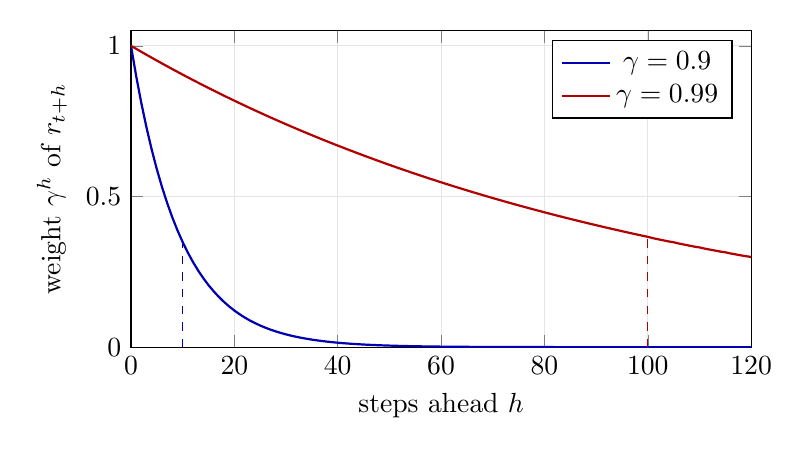
\begin{tikzpicture}
\begin{axis}[width=0.78\linewidth, height=5.6cm, xmin=0, xmax=120, ymin=0, ymax=1.05, xlabel={steps ahead $h$}, ylabel={weight $\gamma^h$ of $r_{t+h}$},
  legend pos=north east, grid=both, grid style={gray!20}]
\addplot[blue!70!black, thick, domain=0:120, samples=121] {0.9^x};
\addplot[red!70!black, thick, domain=0:120, samples=121] {0.99^x};
\addplot[blue!70!black, dashed] coordinates {(10,0)(10,0.349)};
\addplot[red!70!black, dashed] coordinates {(100,0)(100,0.366)};
\legend{$\gamma=0.9$, $\gamma=0.99$}
\end{axis}
\end{tikzpicture}
\caption{Weight of the reward received $h$ steps ahead (original figure; slide 7 only describes this in prose). Dashed lines mark the effective horizon $1/(1-\gamma)$, where the weight has dropped to about $e^{-1}\approx0.37$.}
\label{fig:discount}
\end{figure}

\begin{intuition}
Think of $\gamma$ as a ``patience'' dial. With $\gamma=0.9$ rewards more than $\sim10$ steps away barely matter; with $\gamma=0.99$ the agent looks $\sim100$ steps ahead. The same number $1/(1-\gamma)$ reappears in this lecture as (i) the largest possible value, (ii) the initialisation range for the iterations, and (iii) the factor that inflates the error of the greedy policy. Larger $\gamma$ means a longer horizon and harder computation.
\end{intuition}

\subsection{Bellman Expectation Equation \slide{8}}
The value of a state is expanded in terms of the current reward and the value of the next states, according to the policy:
\begin{align*}
V^\pi(s)&=r(s,\pi(s))+\gamma\,\E_{s'\sim p(\cdot\mid s,\pi(s))}\big[V^\pi(s')\big],\\
Q^\pi(s,a)&=r(s,a)+\gamma\,\E_{s'\sim p(\cdot\mid s,a)}\big[V^\pi(s')\big],\qquad V^\pi(s)=Q^\pi(s,\pi(s)).
\end{align*}
In the first line the reward is a function of $s$ and $\pi(s)$; in the second, of $s$ and $a$.

\begin{fact}[L03-1, Theorem 6 --- Bellman expectation equation]\label{fact:bexp}
For every policy $\pi$ and every state $s$, the display above holds. In operator language (Definition~\ref{def:bellman}): $\Bpi V^\pi=V^\pi$.
\end{fact}

\begin{intuition}
A one-step lookahead: \emph{what you get now} plus \emph{the discounted value of wherever you land}, averaged over the randomness of the transition. It turns an infinite sum into a \emph{local} consistency condition that must hold in all states simultaneously, and that is exactly what we will exploit to compute $V^\pi$.
\end{intuition}

\subsection{Bellman Optimality \slides{9--12}}
\textbf{Example (slide 9).} Suppose we already know $V^*$ at the successor states $s'$ and $s''$. From $s$ we try each action: taking $a'$ gives reward $r(s,a')$ and leads to $s'$, so $Q^*(s,a')=r(s,a')+\gamma V^*(s')$; likewise $Q^*(s,a'')=r(s,a'')+\gamma V^*(s'')$. Then $V^*(s)=\max\{Q^*(s,a'),Q^*(s,a'')\}$ (\figref{fig:tree}; the slide draws deterministic transitions, with stochastic ones $V^*(s')$ becomes an expectation).

\begin{figure}[htbp]
\centering
\begin{tikzpicture}
  \node[st] (s) at (0,0) {$s$};
  \node[st] (s1) at (-2.2,-2.2) {$s'$};
  \node[st] (s2) at (2.2,-2.2) {$s''$};
  \draw[->, thick] (s) -- node[left, pos=0.45] {$a'$} (s1);
  \draw[->, thick] (s) -- node[right, pos=0.45] {$a''$} (s2);
  \node[align=left, anchor=west] at (3.6,-0.6) {$Q^*(s,a')=r(s,a')+\gamma V^*(s')$\\[3pt] $Q^*(s,a'')=r(s,a'')+\gamma V^*(s'')$};
  \node at (0,-3.4) {$V^*(s)=\max\{\,Q^*(s,a'),\,Q^*(s,a'')\,\}$};
\end{tikzpicture}
\caption{Bellman optimality backup in one picture (redrawn from slide 9): try every action, evaluate it with the (assumed known) values of the successors, keep the best.}
\label{fig:tree}
\end{figure}

In general,
\[
V^*(s)=\max_a\Big[r(s,a)+\gamma\,\E_{s'\sim p(\cdot\mid s,a)}V^*(s')\Big],\qquad
Q^*(s,a)=r(s,a)+\gamma\,\E_{s'\sim p(\cdot\mid s,a)}\Big[\max_{a'}Q^*(s',a')\Big].
\]
Two results from L03 are quoted on the slides:

\begin{fact}[Slide 10 ``Theorem 1'', L03-1 Theorem 8 --- Bellman optimality]\label{fact:bopt}
$V^*$ and $Q^*$ satisfy the two equations above, and the greedy policy $\hat\pi(s)\in\argmax_aQ^*(s,a)$ satisfies $V^{\hat\pi}=V^*$. Hence $\pi^*(s)=\argmax_aQ^*(s,a)$ is an optimal policy.
\end{fact}

\begin{fact}[Slide 11 ``Theorem 2'', L03-1 Theorem 10 --- uniqueness]\label{fact:uniq}
For any $V$, if $V(s)=\max_a\big[r(s,a)+\gamma\E_{s'\sim p(\cdot\mid s,a)}V(s')\big]$ for all $s$, then $V=V^*$.
\end{fact}

\begin{intuition}
The optimality equation lets us \emph{focus on one step at a time}: we only choose the best first action and leave the rest of the problem to $V(s')$. Fact~\ref{fact:uniq} says that any function that is locally self-consistent in this sense \emph{is} $V^*$: there is nothing else to look for. Fact~\ref{fact:bopt} converts $Q^*$ into a policy by a plain $\argmax$. Together they say: \emph{find the unique solution of the Bellman optimality equation and you are done}. How to find it is the subject of the rest of the lecture. (The proof of uniqueness in L03 was a long unrolling argument; Corollary~\ref{cor:fixed} below re-proves it in one line.) \slide{12} closes the recap.
\end{intuition}
%=====================================================================
\section{Policy Evaluation \slides{13--15}}
%=====================================================================
\textbf{Question.} Given an MDP $(\cS,\cA,p,r,\gamma)$ and a policy $\pi$, how can we compute the goodness of $\pi$, i.e.\ $V^\pi$?

\textbf{Why is this interesting?} There are $|\cA|^{|\cS|}$ possible deterministic policies, and we want to find the optimal one. To find it, we need to be able to \emph{evaluate} candidates.

\begin{intuition}
Policy evaluation is the ``scoring function'' of reinforcement learning: before you can say that one policy is better than another you need a number (really, a vector with one entry per state) that says how well each one does. Everything in this lecture is about computing such numbers cheaply: first for a \emph{given} policy, then for the \emph{best} policy at once.
\end{intuition}

%=====================================================================
\section{Exact Policy Evaluation \slides{16--22}}\label{sec:exact}
%=====================================================================
\emph{Note: the companion note marks this block as ``on the slides only'': it is not proved there, so prepare it from the slides.}

Given $(\cS,\cA,p,r,\gamma)$ and $\pi$, what is $V^\pi$? We know that the Bellman expectation equation holds for \emph{all} states:
\[
V^\pi(s)=r(s,\pi(s))+\gamma\sum_{s'\in\cS}p(s'\mid s,\pi(s))\,V^\pi(s').
\]
\emph{How many linear constraints do we have?} $|\cS|$, one per state, in the $|\cS|$ unknowns $V^\pi(s)$. We can combine all the constraints (slide credit: Wen Sun). Define the reward vector and the transition matrix induced by $\pi$:
\[
r^\pi\in\R^{|\cS|},\ (r^\pi)_s=r(s,\pi(s));\qquad
P^\pi\in\R^{|\cS|\times|\cS|},\ (P^\pi)_{s,s'}=p(s'\mid s,\pi(s)).
\]
Then the $|\cS|$ equations read $V^\pi=r^\pi+\gamma P^\pi V^\pi$ (\figref{fig:matrix}), which we can solve for $V^\pi$.

\begin{figure}[htbp]
\centering
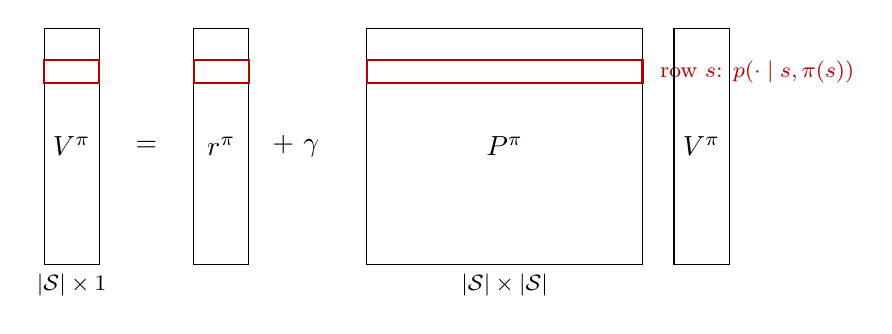
\begin{tikzpicture}[x=1cm,y=1cm]
  % V
  \draw (0,0) rectangle (0.7,3); \node at (0.35,1.5) {$V^\pi$};
  \node at (1.3,1.5) {$=$};
  \draw (1.9,0) rectangle (2.6,3); \node at (2.25,1.5) {$r^\pi$};
  \node at (3.2,1.5) {$+\ \gamma$};
  \draw (4.1,0) rectangle (7.6,3); \node at (5.85,1.5) {$P^\pi$};
  \draw[red!70!black, thick] (4.1,2.3) rectangle (7.6,2.6);
  \node[red!70!black, font=\footnotesize, anchor=west] at (7.7,2.45) {row $s$: $p(\cdot\mid s,\pi(s))$};
  \draw (8.0,0) rectangle (8.7,3); \node at (8.35,1.5) {$V^\pi$};
  \draw[red!70!black, thick] (0,2.3) rectangle (0.7,2.6);
  \draw[red!70!black, thick] (1.9,2.3) rectangle (2.6,2.6);
  \node[font=\footnotesize, below] at (0.35,0) {$|\cS|\times1$};
  \node[font=\footnotesize, below] at (5.85,0) {$|\cS|\times|\cS|$};
\end{tikzpicture}
\caption{The $|\cS|$ Bellman expectation equations stacked in matrix form (redrawn from slides 20--22). The highlighted row is the equation for one state $s$: $V^\pi(s)=r(s,\pi(s))+\gamma\,\langle p(\cdot\mid s,\pi(s)),V^\pi\rangle$.}
\label{fig:matrix}
\end{figure}

\begin{proposition}[Exact policy evaluation, slides 21--22]\label{prop:exact}
For $\gamma<1$, the matrix $I-\gamma P^\pi$ is invertible and
\[
V^\pi=(I-\gamma P^\pi)^{-1}r^\pi=\sum_{k\ge0}\gamma^k(P^\pi)^kr^\pi .
\]
Computing it by matrix inversion costs $O(|\cS|^3)$.
\end{proposition}
\begin{proof}
$P^\pi$ is row-stochastic (entries $\ge0$, each row sums to $1$), so its induced $\infty$-norm is $1$ and $\norm{\gamma P^\pi x}\le\gamma\norm{x}$. If $(I-\gamma P^\pi)x=0$ then $x=\gamma P^\pi x$, so $\norm{x}\le\gamma\norm{x}$, forcing $x=0$ since $\gamma<1$; hence the matrix is invertible. The Neumann series $\sum_k(\gamma P^\pi)^k$ converges (its terms have norm $\le\gamma^k$) and equals the inverse. Rearranging $V^\pi=r^\pi+\gamma P^\pi V^\pi$ gives $(I-\gamma P^\pi)V^\pi=r^\pi$. Inverting an $|\cS|\times|\cS|$ matrix takes $O(|\cS|^3)$ operations.
\end{proof}

\begin{intuition}
The Neumann series is the Bellman equation unrolled: $(P^\pi)^kr^\pi$ is the expected reward $k$ steps ahead, and $\gamma^k$ discounts it, so $V^\pi$ is literally the \emph{expected discounted sum of rewards}. The closed form is ``nice but computationally expensive'' (the slide's own verdict): cubic in the number of states is fine for dozens of states but hopeless for millions. This motivates an approach that only needs matrix--vector products.
\end{intuition}

\begin{example}[A two-state MDP, used throughout]\label{ex:toy}
Take $\cS=\{s_1,s_2\}$, $\cA=\{a,b\}$, $\gamma=0.9$, with
\begin{center}
\begin{tabular}{@{}lccc@{}}
\toprule
$(s,\text{action})$ & $r$ & $p(s_1\mid\cdot)$ & $p(s_2\mid\cdot)$\\
\midrule
$(s_1,a)$ & $0$ & $0.5$ & $0.5$\\
$(s_1,b)$ & $0.5$ & $1$ & $0$\\
$(s_2,a)$ & $1$ & $0.1$ & $0.9$\\
$(s_2,b)$ & $0.2$ & $1$ & $0$\\
\bottomrule
\end{tabular}
\end{center}
\begin{center}
\begin{tikzpicture}[scale=0.95]
  \node[font=\footnotesize, gray] at (0,3.5) {state};
  \node[font=\footnotesize, gray] at (4.2,3.5) {action};
  \node[font=\footnotesize, gray] at (8.4,3.5) {next state};
  \node[st] (s1) at (0,1.6) {$s_1$};
  \node[st] (s2) at (0,-1.6) {$s_2$};
  \node[act] (a1) at (4.2,2.5) {};
  \node[act] (b1) at (4.2,0.9) {};
  \node[act] (a2) at (4.2,-0.9) {};
  \node[act] (b2) at (4.2,-2.5) {};
  \node[st] (t1) at (8.4,1.6) {$s_1$};
  \node[st] (t2) at (8.4,-1.6) {$s_2$};
  \draw (s1) -- node[above, sloped, font=\scriptsize, pos=0.5] {$a,\ r{=}0$} (a1);
  \draw (s1) -- node[below, sloped, font=\scriptsize, pos=0.5] {$b,\ r{=}0.5$} (b1);
  \draw (s2) -- node[above, sloped, font=\scriptsize, pos=0.5] {$a,\ r{=}1$} (a2);
  \draw (s2) -- node[below, sloped, font=\scriptsize, pos=0.5] {$b,\ r{=}0.2$} (b2);
  \draw[->] (a1) -- node[fill=white, inner sep=1pt, font=\scriptsize, pos=0.6] {$0.5$} (t1);
  \draw[->] (a1) -- node[fill=white, inner sep=1pt, font=\scriptsize, pos=0.25] {$0.5$} (t2);
  \draw[->] (b1) -- node[fill=white, inner sep=1pt, font=\scriptsize, pos=0.6] {$1$} (t1);
  \draw[->] (a2) -- node[fill=white, inner sep=1pt, font=\scriptsize, pos=0.25] {$0.1$} (t1);
  \draw[->] (a2) -- node[fill=white, inner sep=1pt, font=\scriptsize, pos=0.6] {$0.9$} (t2);
  \draw[->] (b2) -- node[fill=white, inner sep=1pt, font=\scriptsize, pos=0.15] {$1$} (t1);
\end{tikzpicture}
\end{center}
Filled dots are state-action pairs; the arrows leaving a dot are the stochastic transitions, labelled with their probabilities. For the policy $\pi=(a,a)$ (always play $a$):
\[
P^\pi=\begin{pmatrix}0.5&0.5\\0.1&0.9\end{pmatrix},\quad r^\pi=\begin{pmatrix}0\\1\end{pmatrix},\quad
I-\gamma P^\pi=\begin{pmatrix}0.55&-0.45\\-0.09&0.19\end{pmatrix},\quad \det=0.064,
\]
\[
V^\pi=(I-\gamma P^\pi)^{-1}r^\pi=\frac1{0.064}\begin{pmatrix}0.19&0.45\\0.09&0.55\end{pmatrix}\begin{pmatrix}0\\1\end{pmatrix}
=\begin{pmatrix}7.03125\\8.59375\end{pmatrix}.
\]
It will turn out that this policy is in fact optimal for this MDP: $V^*=(7.03125,\,8.59375)$.
\end{example}

%=====================================================================
\section{Fixed-Point Iteration \slides{23--24}}
%=====================================================================
What is a \textbf{fixed point}? A point $x$ such that $x=f(x)$. How can we find such points?
\begin{enumerate}[label=\arabic*.]
  \item Initialise $x_0$.
  \item Repeat $x_{i+1}=f(x_i)$.
  \item Stop at convergence, when $x$ does not change any more.
\end{enumerate}
Geometrically (slide 24), fixed points are the intersections of $y=f(x)$ with the line $y=x$. The iteration is a ``cobweb'': from $(x_i,x_i)$ on the diagonal go vertically to the curve at $(x_i,x_{i+1})$, then horizontally back to the diagonal at $(x_{i+1},x_{i+1})$. The slide's example is $f(x)=\cos x$, with fixed point $x^*\approx0.739085$.

\begin{figure}[htbp]
\centering
\begin{minipage}{0.52\linewidth}
\centering
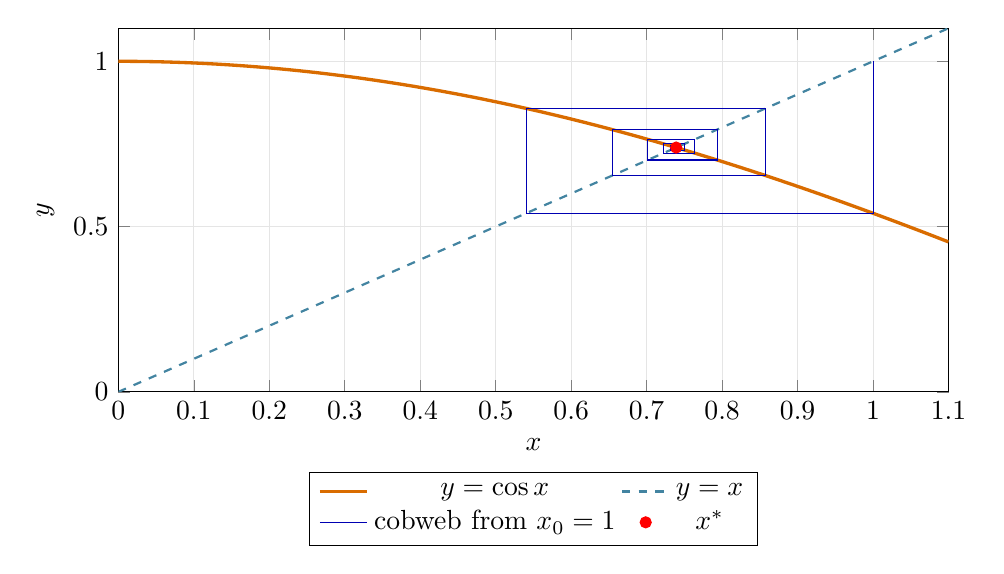
\begin{tikzpicture}
\begin{axis}[width=\linewidth, height=6.2cm, xmin=0, xmax=1.1, ymin=0, ymax=1.1, xlabel={$x$}, ylabel={$y$}, legend style={at={(0.5,-0.22)}, anchor=north, legend columns=2}, grid=both, grid style={gray!20}]
\addplot[orange!85!black, very thick, domain=0:1.1, samples=60] {cos(deg(x))};
\addplot[cyan!60!black, dashed, thick, domain=0:1.1] {x};
\addplot[blue!70!black, thin] coordinates {(1.000000,1.000000) (1.000000,0.540302) (0.540302,0.540302) (0.540302,0.540302) (0.540302,0.857553) (0.857553,0.857553) (0.857553,0.857553) (0.857553,0.654290) (0.654290,0.654290) (0.654290,0.654290) (0.654290,0.793480) (0.793480,0.793480) (0.793480,0.793480) (0.793480,0.701369) (0.701369,0.701369) (0.701369,0.701369) (0.701369,0.763960) (0.763960,0.763960) (0.763960,0.763960) (0.763960,0.722102) (0.722102,0.722102) (0.722102,0.722102) (0.722102,0.750418) (0.750418,0.750418) (0.750418,0.750418) (0.750418,0.731404) (0.731404,0.731404) (0.731404,0.731404) (0.731404,0.744237) (0.744237,0.744237) (0.744237,0.744237) (0.744237,0.735605) (0.735605,0.735605) (0.735605,0.735605) (0.735605,0.741425) (0.741425,0.741425) (0.741425,0.741425) (0.741425,0.737507) (0.737507,0.737507) (0.737507,0.737507) (0.737507,0.740147) (0.740147,0.740147) (0.740147,0.740147) (0.740147,0.738369) (0.738369,0.738369)};
\addplot[only marks, mark=*, red, mark size=2pt] coordinates {(0.739085,0.739085)};
\legend{$y=\cos x$, $y=x$, cobweb from $x_0=1$, $x^*$}
\end{axis}
\end{tikzpicture}
\end{minipage}\hfill
\begin{minipage}{0.45\linewidth}
\centering
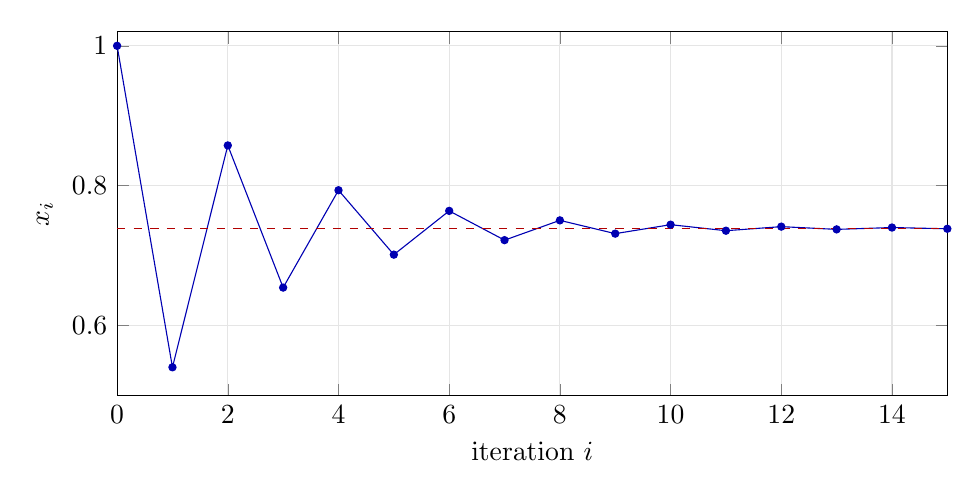
\begin{tikzpicture}
\begin{axis}[width=\linewidth, height=6.2cm, xmin=0, xmax=15, ymin=0.5, ymax=1.02, xlabel={iteration $i$}, ylabel={$x_i$}, grid=both, grid style={gray!20}]
\addplot[blue!70!black, mark=*, mark size=1.3pt] coordinates {(0.000000,1.000000) (1.000000,0.540302) (2.000000,0.857553) (3.000000,0.654290) (4.000000,0.793480) (5.000000,0.701369) (6.000000,0.763960) (7.000000,0.722102) (8.000000,0.750418) (9.000000,0.731404) (10.000000,0.744237) (11.000000,0.735605) (12.000000,0.741425) (13.000000,0.737507) (14.000000,0.740147) (15.000000,0.738369)};
\addplot[red!70!black, dashed] coordinates {(0,0.739085)(15,0.739085)};
\end{axis}
\end{tikzpicture}
\end{minipage}
\caption{Fixed-point iteration of $f(x)=\cos x$ from $x_0=1$ (original figure in the style of slide 24; values computed exactly). Left: cobweb diagram. Right: $x_i\to x^*\approx0.739085$.}
\label{fig:cobweb}
\end{figure}

\begin{intuition}
Fixed-point iteration is ``keep applying the rule until it stops changing anything''. Whether this works depends on the rule: with $f(x)=\cos x$ each step lands closer to $x^*$ (the cobweb spirals in), but for $f(x)=2x$ the iterates would run away from the fixed point $0$. The property that guarantees spiralling \emph{in} is that $f$ brings any two points closer together, which is exactly what the next section calls a contraction.
\end{intuition}
%=====================================================================
\section{Contractions \slides{25--28}}\label{sec:contr}
%=====================================================================
Convergence to a fixed point is possible thanks to the existence of \textbf{contraction mappings}.

\pdfnum{1}
\begin{definition}[Contraction]\label{def:contraction}
Let $(M,d)$ be a metric space. An operator $f:M\to M$ is a \emph{$k$-contraction} if there is $k\in[0,1)$ with
\[
d\big(f(x),f(y)\big)\le k\,d(x,y)\qquad\text{for all }x,y\in M .
\]
(On the slides: $\abs{f(x)-f(x')}\le k\abs{x-x'}$ for $k\in[0,1)$.)
\end{definition}

\pdfnum{2}
\begin{theorem}[Banach fixed-point theorem]\label{thm:banach}
A $k$-contraction on a non-empty \emph{complete} metric space has \emph{exactly one} fixed point $x^*$, and for any starting point $x_0$ the iteration $x_{i+1}=f(x_i)$ converges to it, with $d(x_i,x^*)\le k^i\,d(x_0,x^*)$.
\end{theorem}
\begin{proof}[Proof of uniqueness (this is the part on slide 25: ``a contraction mapping has at most one fixed point'')]
If $f(x)=x$ and $f(y)=y$ then $d(x,y)=d(f(x),f(y))\le k\,d(x,y)$, and since $k<1$ this forces $d(x,y)=0$, i.e.\ $x=y$.
\end{proof}
\emph{The existence of a fixed point, the convergence of the iteration and the rate $k^i$ are not proved on the slides; their proof is in Appendix~\ref{app:banach} (supplementary).}

\begin{intuition}
A contraction is a map that \emph{squeezes space}: any two points end up closer together after one application, by a factor of at least $k<1$. Two fixed points would stay at the same distance after applying $f$, which contradicts the squeezing, so there is at most one. Iterating $f$ keeps squeezing the whole space towards a single point, which is the fixed point; completeness just guarantees that this point exists inside the space instead of being a ``hole''. The rate $k^i$ is the geometric decay that all later bounds inherit.
\end{intuition}

\begin{figure}[htbp]
\centering
\begin{minipage}{0.52\linewidth}
\centering
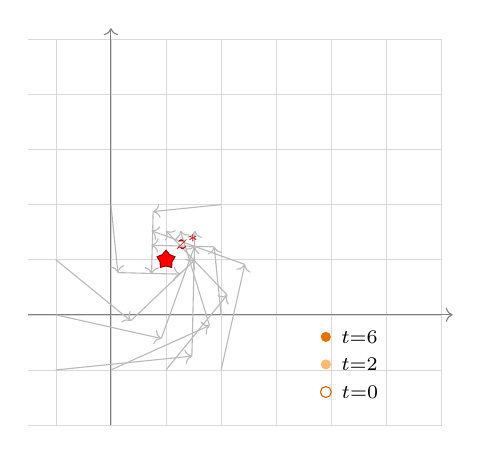
\begin{tikzpicture}[scale=0.7,
  c0/.style={circle, draw=orange!80!black, fill=white, inner sep=1.4pt},
  c2/.style={circle, fill=orange!55, inner sep=1.3pt},
  c6/.style={circle, fill=orange!90!black, inner sep=1.3pt}]
\draw[gray!30, very thin] (-1.5,-2) grid (6,5);
\draw[->, gray] (-1.5,0) -- (6.2,0); \draw[->, gray] (0,-2) -- (0,5.2);
\draw[->, gray!55] (-1.000,-1.000) -- (1.469,-0.749);
\draw[->, gray!55] (0.000,-1.000) -- (1.789,-0.194);
\draw[->, gray!55] (1.000,-1.000) -- (2.109,0.360);
\draw[->, gray!55] (2.000,-1.000) -- (2.429,0.914);
\draw[->, gray!55] (-1.000,0.000) -- (0.914,-0.429);
\draw[->, gray!55] (2.000,0.000) -- (1.874,1.234);
\draw[->, gray!55] (-1.000,1.000) -- (0.360,-0.109);
\draw[->, gray!55] (0.000,2.000) -- (0.126,0.766);
\draw[->, gray!55] (2.000,2.000) -- (0.766,1.874);
\draw[->, gray!55] (1.469,-0.749) -- (1.524,1.524);
\draw[->, gray!55] (1.789,-0.194) -- (1.262,1.524);
\draw[->, gray!55] (2.109,0.360) -- (1.000,1.524);
\draw[->, gray!55] (2.429,0.914) -- (0.738,1.524);
\draw[->, gray!55] (0.914,-0.429) -- (1.524,1.262);
\draw[->, gray!55] (1.874,1.234) -- (0.738,1.262);
\draw[->, gray!55] (0.360,-0.109) -- (1.524,1.000);
\draw[->, gray!55] (0.126,0.766) -- (1.262,0.738);
\draw[->, gray!55] (0.766,1.874) -- (0.738,0.738);
\node[star, star points=5, fill=red, draw=red!60!black, inner sep=1.6pt] at (1,1) {};
\node[red!70!black, font=\footnotesize, above right] at (1,1) {$z^*$};
\node[c0, label={[font=\scriptsize]right:$t{=}0$}] at (3.9,-1.4) {};
\node[c2, label={[font=\scriptsize]right:$t{=}2$}] at (3.9,-0.9) {};
\node[c6, label={[font=\scriptsize]right:$t{=}6$}] at (3.9,-0.4) {};
\end{tikzpicture}
\end{minipage}\hfill
\begin{minipage}{0.45\linewidth}
\centering
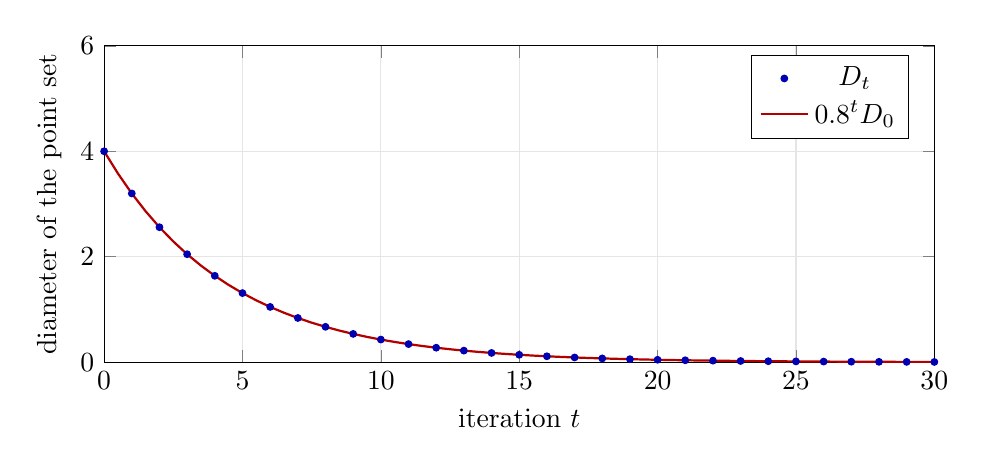
\begin{tikzpicture}
\begin{axis}[width=\linewidth, height=5.6cm, xmin=0, xmax=30, ymin=0, ymax=6, xlabel={iteration $t$}, ylabel={diameter of the point set}, grid=both, grid style={gray!20}, legend pos=north east]
\addplot[only marks, mark=*, mark size=1.2pt, blue!70!black] coordinates {(0.000000,4.000000) (1.000000,3.200000) (2.000000,2.560000) (3.000000,2.048000) (4.000000,1.638400) (5.000000,1.310720) (6.000000,1.048576) (7.000000,0.838861) (8.000000,0.671089) (9.000000,0.536871) (10.000000,0.429497) (11.000000,0.343597) (12.000000,0.274878) (13.000000,0.219902) (14.000000,0.175922) (15.000000,0.140737) (16.000000,0.112590) (17.000000,0.090072) (18.000000,0.072058) (19.000000,0.057646) (20.000000,0.046117) (21.000000,0.036893) (22.000000,0.029515) (23.000000,0.023612) (24.000000,0.018889) (25.000000,0.015112) (26.000000,0.012089) (27.000000,0.009671) (28.000000,0.007737) (29.000000,0.006190) (30.000000,0.004952)};
\addplot[red!70!black, thick, domain=0:30, samples=61] {4*0.8^x};
\legend{$D_t$, $0.8^t D_0$}
\end{axis}
\end{tikzpicture}
\end{minipage}
\caption{A contraction in $\R^2$ (original figure in the style of slide 26): $f(z)=0.8\,R_{30^\circ}z+c$ with unique fixed point $z^*$. Left: nine starting points and their images after $2$ and $6$ steps all collapse onto $z^*$. Right: the diameter of the point set decays exactly like $k^tD_0$ (here $f$ is a similarity, so the contraction inequality is tight).}
\label{fig:contraction}
\end{figure}

\begin{example}[{Why $\cos$ is a contraction on $[0,1]$}]\label{ex:cos}
\emph{(Added example connecting the cobweb of slide 24 to Banach's theorem; not on the slides.)} On $M=[0,1]$ (complete) $\cos$ maps into $[\cos1,1]\approx[0.540,1]\subset M$, and by the mean value theorem $\abs{\cos x-\cos y}=\abs{\sin\xi}\,\abs{x-y}\le\sin(1)\,\abs{x-y}$ with $\sin 1\approx0.841$. So $\cos$ is a $0.841$-contraction on $[0,1]$; Theorem~\ref{thm:banach} gives a unique fixed point ($x^*\approx0.739085$) and $\abs{x_i-x^*}\le0.841^i\abs{x_0-x^*}$. In \figref{fig:cobweb}, $x_0=1$ gives $\abs{x_5-x^*}\approx0.038$, comfortably below the bound $0.841^5\cdot0.261\approx0.110$.
\end{example}

\subsection{Contraction Operator \slides{27--28}}
In the simplest case the contraction can be an \emph{operator}, even as simple as a matrix $O$ acting on value vectors:
\[
\abs{OV-OV'}\le\gamma\abs{V-V'}
\]
(we can write $\gamma$ instead of $k$, since both lie in $[0,1)$). The slide's demo takes $O=\gamma I$, ``pure shrink'': every vector is scaled by $\gamma$, so the distance between $OV$ and $OV'$ is exactly $\gamma$ times the distance between $V$ and $V'$ (\figref{fig:operator}).

\begin{figure}[htbp]
\centering
\begin{minipage}{0.55\linewidth}
\centering
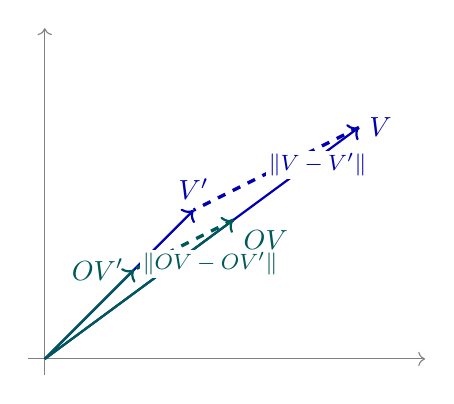
\begin{tikzpicture}[scale=1.05]
\draw[->, gray] (-0.2,0) -- (4.6,0); \draw[->, gray] (0,-0.2) -- (0,4.0);
\coordinate (V) at (3.8,2.8); \coordinate (W) at (1.8,1.8);
\coordinate (OV) at (2.28,1.68); \coordinate (OW) at (1.08,1.08);
\draw[->, thick, blue!70!black] (0,0) -- (V) node[right] {$V$};
\draw[->, thick, blue!70!black] (0,0) -- (W) node[above] {$V'$};
\draw[->, thick, teal!70!black] (0,0) -- (OV) node[below right] {$OV$};
\draw[->, thick, teal!70!black] (0,0) -- (OW) node[left] {$OV'$};
\draw[dashed, blue!70!black, very thick] (V) -- (W);
\draw[dashed, teal!70!black, very thick] (OV) -- (OW);
\node[blue!70!black, font=\footnotesize, fill=white, inner sep=1pt] at (3.3,2.35) {$\lVert V-V'\rVert$};
\node[teal!70!black, font=\footnotesize, fill=white, inner sep=1pt] at (2.0,1.15) {$\lVert OV-OV'\rVert$};
\end{tikzpicture}
\end{minipage}\hfill
\begin{minipage}{0.4\linewidth}
\centering
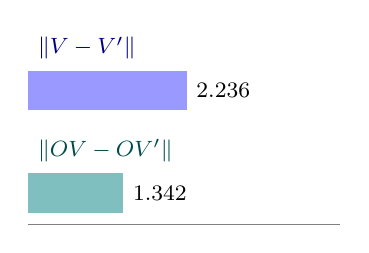
\begin{tikzpicture}[x=0.9cm]
  \fill[blue!40] (0,1.6) rectangle (2.236,2.1);
  \fill[teal!50] (0,0.3) rectangle (1.342,0.8);
  \node[anchor=west, font=\footnotesize] at (2.236,1.85) {2.236};
  \node[anchor=west, font=\footnotesize] at (1.342,0.55) {1.342};
  \node[anchor=south west, font=\footnotesize, blue!50!black] at (0,2.12) {$\lVert V-V'\rVert$};
  \node[anchor=south west, font=\footnotesize, teal!60!black] at (0,0.82) {$\lVert OV-OV'\rVert$};
  \draw[gray] (0,0.15) -- (4.4,0.15);
\end{tikzpicture}
\end{minipage}
\caption{Contraction operator $O=\gamma I$ with $\gamma=0.6$ (original figure in the style of slide 28; Euclidean norm). Applying $O$ shrinks the distance between any two value vectors from $2.236$ to $1.342=0.6\times2.236$.}
\label{fig:operator}
\end{figure}

\begin{intuition}
The point of this slide is the \emph{reading} of ``contraction'' for value functions: think of each value function as a point in $\R^{|\cS|}$ (one coordinate per state); an operator is a contraction when it makes two different value functions \emph{more similar}. The Bellman backups we are about to study are not as trivial as $\gamma I$, but they shrink distances in the same way, by at least a factor $\gamma$ in sup-norm.
\end{intuition}

%=====================================================================
\section{Iterative Policy Evaluation \slides{29--32}}\label{sec:itpe}
%=====================================================================
Instead of inverting a matrix, we exploit the fixed-point structure $V^\pi=r^\pi+\gamma P^\pi V^\pi$ and \emph{iterate} it. We assume rewards are in $[0,1]$.

\begin{algorithm}[Iterative policy evaluation]\label{alg:pe}
\emph{Input:} an MDP $(\cS,\cA,p,r,\gamma)$ and a policy $\pi$.\par
\begin{enumerate}[label=\arabic*.,leftmargin=*]
  \item Initialise $V_0\in[0,1/(1-\gamma)]^{|\cS|}$ (typically $V_0=0$).
  \item Until convergence: $V_{i+1}=r^\pi+\gamma P^\pi V_i$ \quad (matrix form: all states are updated at once).
\end{enumerate}
In operator notation, $V_{i+1}=\Bpi V_i$: this is the \emph{Bellman expectation backup}.
\end{algorithm}
(In the companion note: ``repeat $V_{i+1}=\Bpi V_i$ until $\norm{V_{i+1}-V_i}$ is small.'')

\textbf{Why initialise in $[0,1/(1-\gamma)]$?} Under the assumption $r(s,a)\in[0,1]$, the maximum possible value is $1+\gamma+\gamma^2+\dots=1/(1-\gamma)$ (Fact~\ref{fact:range}). There is no reason to initialise higher than that, since no true value lives there.

\pdfnum{3}
\begin{definition}[Bellman operators]\label{def:bellman}
For a policy $\pi$, a value function $V$ and a state-action function $Q$:
\begin{align*}
(\Bpi V)(s)&=r(s,\pi(s))+\gamma\,\E_{s'\sim p(\cdot\mid s,\pi(s))}\big[V(s')\big] &&\text{(expectation backup, slide 32)},\\
(\Bell V)(s)&=\max_a\Big[r(s,a)+\gamma\,\E_{s'\sim p(\cdot\mid s,a)}\big[V(s')\big]\Big] &&\text{(optimality backup, slide 44)},\\
(\Bell Q)(s,a)&=r(s,a)+\gamma\,\E_{s'\sim p(\cdot\mid s,a)}\Big[\max_{a'}Q(s',a')\Big] &&\text{(on $Q$, slide 48)}.
\end{align*}
$\Bpi$ is \emph{affine} ($\Bpi V=r^\pi+\gamma P^\pi V$); $\Bell$ is \emph{not} linear, because of the maximum. (Part of the literature writes $T$ for $\Bell$.)
\end{definition}

\begin{intuition}
A ``backup'' is one round of ``look one step ahead and update''. The expectation backup $\Bpi$ asks: \emph{if I act according to $\pi$ for one step and then trust my current guess $V$, what is the value of each state?} The optimality backup $\Bell$ asks the same but lets me \emph{pick the best action} in the first step. Facts~\ref{fact:bexp} and \ref{fact:bopt} say precisely that $V^\pi$ and $V^*$ are the states of the world these backups leave untouched.
\end{intuition}

\begin{example}[Iterative evaluation on the two-state MDP]\label{ex:pe}
For $\pi=(a,a)$ in Example~\ref{ex:toy} and $V_0=0$ (so $\norm{V_0-V^\pi}=8.594$):
\begin{center}
\begin{tabular}{@{}rcccc@{}}
\toprule
$i$ & $V_i(s_1)$ & $V_i(s_2)$ & $\norm{V_i-V^\pi}$ & $\gamma^i\norm{V_0-V^\pi}$\\
\midrule
0 & 0.000 & 0.000 & 8.594 & 8.594 \\
1 & 0.000 & 1.000 & 7.594 & 7.734 \\
2 & 0.450 & 1.810 & 6.784 & 6.961 \\
3 & 1.017 & 2.507 & 6.087 & 6.265 \\
4 & 1.586 & 3.122 & 5.472 & 5.638 \\
5 & 2.118 & 3.671 & 4.922 & 5.075 \\
6 & 2.605 & 4.165 & 4.429 & 4.567 \\
7 & 3.046 & 4.608 & 3.986 & 4.110 \\
8 & 3.444 & 5.006 & 3.587 & 3.699 \\
9 & 3.803 & 5.365 & 3.229 & 3.329 \\
10 & 4.126 & 5.688 & 2.906 & 2.996 \\
11 & 4.416 & 5.979 & 2.615 & 2.697 \\
12 & 4.678 & 6.240 & 2.354 & 2.427 \\
13 & 4.913 & 6.476 & 2.118 & 2.184 \\
14 & 5.125 & 6.687 & 1.906 & 1.966 \\
15 & 5.315 & 6.878 & 1.716 & 1.769 \\
\bottomrule
\end{tabular}
\end{center}
The first sweep gives $V_1=r^\pi=(0,1)$; each later sweep propagates reward information one step further. The true error always stays below the geometric bound (last column), as proved next.
\end{example}

%=====================================================================
\section{Iterative Policy Evaluation Theorem \slides{33--37}}\label{sec:thm4}
%=====================================================================
The slides' claim is that, for any two value functions $U$ and $V$ and for all $s\in\cS$,
\[
\abs{(\Bpi U)(s)-(\Bpi V)(s)}\le\gamma\norm{U-V},\qquad\norm{V}=\max_s\abs{V(s)}
\]
(``the largest difference between state values'', worst case scenario to infinity). The companion note packages this together with the analogous claim for $\Bell$ (proved later, slides 44--47):

\pdfnum{4}
\begin{theorem}[Both operators are $\gamma$-contractions in the sup-norm]\label{thm:contraction}
For all value functions $U,V$:
\[
\text{(i)}\ \ \norm{\Bpi U-\Bpi V}\le\gamma\norm{U-V},\qquad
\text{(ii)}\ \ \norm{\Bell U-\Bell V}\le\gamma\norm{U-V}.
\]
The same holds for $\Bell$ acting on state-action functions $Q$.
\end{theorem}
\begin{proof}[Proof of (i), as on slides 33--37]
For $\Bpi$ the rewards cancel. For every state $s$,
\begin{align*}
\abs{(\Bpi U)(s)-(\Bpi V)(s)}
&=\gamma\,\Big|\E_{s'}\big[U(s')-V(s')\big]\Big|\\
&\le\gamma\,\E_{s'}\abs{U(s')-V(s')} &&\text{(Jensen: $\abs{\cdot}$ is convex)}\\
&\le\gamma\,\norm{U-V} &&\text{(an average is at most the maximum).}
\end{align*}
The inequality holds for every $s$, so also for the state where the left-hand side is largest; taking the maximum over $s$ gives (i). The proof of (ii) is in Section~\ref{sec:optcontr}.
\end{proof}

\begin{intuition}
Two things happen in the proof. First, both backups use the \emph{same} rewards, so these cancel: the only thing that differs is the next-state values, scaled by $\gamma$. Second, the next-state values are \emph{averaged} by probabilities that sum to one, and an average of numbers each at most $\norm{U-V}$ in size cannot exceed $\norm{U-V}$. So no state can end up further apart than $\gamma$ times the worst gap before. As the slide remarks, we are not secretly using the sup-norm on the left-hand side: the bound holds \emph{for each state}, including the one with the largest difference.
\end{intuition}

Slide 34 draws the conclusion: \emph{hence the Bellman expectation backup is a contraction mapping and $V^\pi$ is its fixed point}. This follows from Theorem~\ref{thm:banach} applied to $\Bpi$ on $(\R^{|\cS|},\norm{\cdot})$, which is complete (a finite-dimensional normed space): by Fact~\ref{fact:bexp}, $\Bpi V^\pi=V^\pi$, so $V^\pi$ is a fixed point, and by Banach's uniqueness it is the only one. (This is part (a) of Corollary~\ref{cor:fixed}, stated in full in the Value Iteration section.)

%=====================================================================
\section{Iterative Policy Evaluation: Iterations \slide{38}}\label{sec:peiters}
%=====================================================================
\pdfnum{6}
\begin{corollary}[Convergence and cost of iterative policy evaluation]\label{cor:pe}
$\norm{V_i-V^\pi}\le\gamma^i\norm{V_0-V^\pi}$, so $\norm{V_i-V^\pi}\le\epsilon$ after
\[
i\;\ge\;\frac{\ln\!\big(\norm{V_0-V^\pi}/\epsilon\big)}{\ln(1/\gamma)}
\]
iterations, each costing $O(|\cS|^2)$ arithmetic operations. Hence an $\epsilon$-accurate value function costs $O\big(|\cS|^2\ln(1/\epsilon)\big)$ (treating $\gamma$ and $\norm{V_0-V^\pi}$ as constants).
\end{corollary}
\begin{proof}
The rate is Theorem~\ref{thm:banach} with $k=\gamma$, applied to $\Bpi$ whose unique fixed point is $V^\pi$. Solving $\gamma^i\norm{V_0-V^\pi}\le\epsilon$ for $i$ (take logarithms; $\ln\gamma=-\ln(1/\gamma)<0$ flips the inequality) gives the count. Each sweep updates $|\cS|$ states and each update averages over $|\cS|$ successors, i.e.\ one matrix--vector product $P^\pi V_i$.
\end{proof}

\begin{figure}[htbp]
\centering
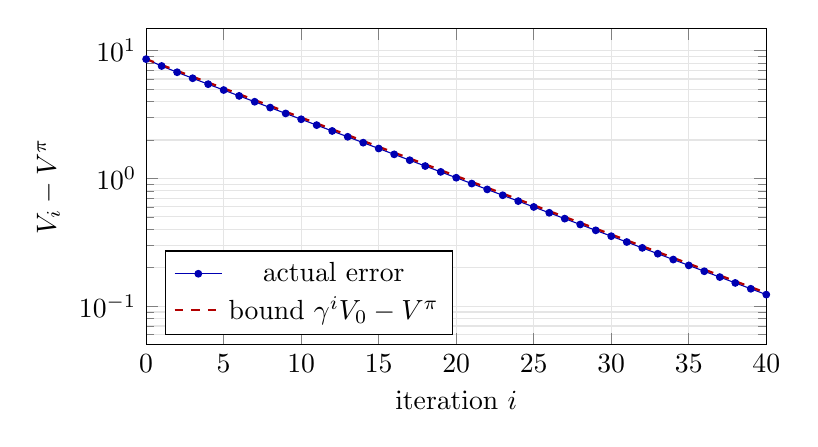
\begin{tikzpicture}
\begin{axis}[width=0.78\linewidth, height=5.6cm, xmin=0, xmax=40, ymode=log, ymin=0.05, ymax=15, xlabel={iteration $i$}, ylabel={$\norm{V_i-V^\pi}$}, grid=both, grid style={gray!20}, legend pos=south west]
\addplot[blue!70!black, mark=*, mark size=1.2pt] coordinates {(0.000000,8.593750) (1.000000,7.593750) (2.000000,6.783750) (3.000000,6.087150) (4.000000,5.471874) (5.000000,4.922325) (6.000000,4.429242) (7.000000,3.986012) (8.000000,3.587300) (9.000000,3.228531) (10.000000,2.905663) (11.000000,2.615092) (12.000000,2.353581) (13.000000,2.118222) (14.000000,1.906400) (15.000000,1.715759) (16.000000,1.544184) (17.000000,1.389765) (18.000000,1.250789) (19.000000,1.125710) (20.000000,1.013139) (21.000000,0.911825) (22.000000,0.820642) (23.000000,0.738578) (24.000000,0.664720) (25.000000,0.598248) (26.000000,0.538423) (27.000000,0.484581) (28.000000,0.436123) (29.000000,0.392511) (30.000000,0.353260) (31.000000,0.317934) (32.000000,0.286140) (33.000000,0.257526) (34.000000,0.231774) (35.000000,0.208596) (36.000000,0.187737) (37.000000,0.168963) (38.000000,0.152067) (39.000000,0.136860) (40.000000,0.123174)};
\addplot[red!70!black, dashed, thick, domain=0:40, samples=41] {8.59375*0.9^x};
\legend{actual error, bound $\gamma^i\norm{V_0-V^\pi}$}
\end{axis}
\end{tikzpicture}
\caption{Iterative policy evaluation on Example~\ref{ex:toy} with $\pi=(a,a)$, $\gamma=0.9$, $V_0=0$. On a log scale the error is a straight line: geometric convergence. The error decays geometrically and remains below the contraction bound.}
\label{fig:pe_err}
\end{figure}

\begin{intuition}
\emph{Worked numbers.} With $\gamma=0.9$, $\epsilon=0.01$ and $\norm{V_0-V^\pi}=8.594$: $i\ge\ln(859.4)/\ln(1/0.9)=6.756/0.1054=64.1$, so $65$ sweeps (indeed $0.9^{65}\cdot8.594\approx0.009$). Each sweep is only $|\cS|^2=4$ multiplications here. The \emph{accuracy} costs only a logarithm ($10\times$ smaller $\epsilon$ adds $\ln 10/\ln(1/\gamma)\approx22$ sweeps), while the \emph{horizon} $\ln(1/\gamma)\approx1-\gamma$ drives the cost. Compared with $O(|\cS|^3)$ for exact evaluation, iteration wins when $|\cS|$ is large and $\epsilon$ is moderate.
\end{intuition}
%=====================================================================
\section{How to Find the Optimal Policy? \slides{39--43}}
%=====================================================================
Now what we are really interested in is finding the optimal policy $\pi^*$.

\textbf{Naive approach} (slides 40--42): we know how to do policy evaluation, so
\begin{itemize}
  \item for each possible policy, for all states,
  \item do policy evaluation and compute $V^\pi(s)$,
  \item choose $\pi'$ such that $V^{\pi'}(s)\ge V^\pi(s)$ (keep the best).
\end{itemize}
If we use exact policy evaluation the cost is $O\big(|\cA|^{|\cS|}\,|\cS|^3\big)$: $|\cA|^{|\cS|}$ policies, each needing a cubic solve.

\begin{intuition}
The slide's horrified emoji is justified. The number of deterministic policies grows \emph{exponentially} in the number of states: for $|\cA|=2$, $|\cS|=10$ there are $1024$ policies (about $10^6$ operations in total), but for $|\cS|=30$ there are $2^{30}\approx10^9$ policies and about $2.9\times10^{13}$ operations. Enumeration treats the policies as unrelated black boxes. The better idea (slide 43): \textbf{let's use the Bellman optimality equation!} Rather than searching over policies, search for the one function $V^*$ (or $Q^*$) that satisfies it, and read the policy off with an $\argmax$ (Fact~\ref{fact:bopt}).
\end{intuition}

%=====================================================================
\section{The Bellman Optimality Backup is a Contraction \slides{44--47}}\label{sec:optcontr}
%=====================================================================
Set $\gamma<1$ and use the sup-norm $\norm{V}=\max_s\abs{V(s)}$. Define the (non-linear) operator $\Bell V$ as the Bellman optimality equation applied to $V$ (Definition~\ref{def:bellman}):
\[
(\Bell V)(s)=\max_a\Big[r(s,a)+\gamma\sum_{s'\in\cS}p(s'\mid s,a)\,V(s')\Big].
\]
We need one elementary fact about maxima, used implicitly on the slides:

\begin{lemma}[The maximum is 1-Lipschitz]\label{lem:max}
For any two functions $f,g$ on a finite set of actions, $\big|\max_af(a)-\max_ag(a)\big|\le\max_a\abs{f(a)-g(a)}$.
\end{lemma}
\begin{proof}
Let $a_f$ attain $\max_af$. Then $\max_af-\max_ag\le f(a_f)-g(a_f)\le\max_a\abs{f(a)-g(a)}$. Exchanging the roles of $f$ and $g$ gives the other sign.
\end{proof}

\begin{proof}[Proof of Theorem~\ref{thm:contraction}\,(ii), following slides 45--47]
Fix two value functions $V_k,V_j$ and a state $s$. Using Lemma~\ref{lem:max} with $f(a)=r(s,a)+\gamma\sum_{s'}p(s'\mid s,a)V_k(s')$ and $g$ the same with $V_j$, the reward terms cancel:
\begin{align*}
\big|(\Bell V_k)(s)-(\Bell V_j)(s)\big|
&\le\max_a\Big|\gamma\sum_{s'}p(s'\mid s,a)\big(V_k(s')-V_j(s')\big)\Big|\\
&\le\max_a\gamma\sum_{s'}p(s'\mid s,a)\,\norm{V_k-V_j}\\
&=\gamma\norm{V_k-V_j},
\end{align*}
where the second step bounds each $\abs{V_k(s')-V_j(s')}$ by the sup-norm, and the last equality uses $\sum_{s'}p(s'\mid s,a)=1$. Taking the maximum over $s$ gives $\norm{\Bell V_k-\Bell V_j}\le\gamma\norm{V_k-V_j}$.
\end{proof}

\begin{intuition}
If you apply $\Bell$ to two different value functions, \emph{the distance between them shrinks} (slide 46): $\Bell$ makes value functions closer by at least a factor $\gamma$ (slide 47). The new ingredient compared with the expectation backup is the $\max$, and Lemma~\ref{lem:max} says it cannot amplify differences: changing a few action values by at most $\delta$ changes the best of them by at most $\delta$. So even though $\Bell$ is non-linear, it inherits the same squeezing property as $\Bpi$.
\end{intuition}

%=====================================================================
\section{Bellman Operator for $Q$ \slide{48}}
%=====================================================================
Since $Q:\cS\times\cA\to\R$, also $\Bell Q:\cS\times\cA\to\R$:
\[
(\Bell Q)(s,a)=r(s,a)+\gamma\,\E_{s'\sim p(\cdot\mid s,a)}\Big[\max_{a'}Q(s',a')\Big],
\]
and the norm is now $\norm{Q}=\max_{s,a}\abs{Q(s,a)}$.

\begin{proof}[Proof of the last claim of Theorem~\ref{thm:contraction} (the $Q$-version)]
Rewards cancel, and the maximum now sits \emph{inside} the expectation. For every $(s,a)$,
\[
\abs{(\Bell Q)(s,a)-(\Bell Q')(s,a)}
=\gamma\Big|\E_{s'}\big[\max_{a'}Q(s',a')-\max_{a'}Q'(s',a')\big]\Big|
\le\gamma\,\E_{s'}\max_{a'}\abs{Q(s',a')-Q'(s',a')}
\le\gamma\norm{Q-Q'},
\]
using $\abs{\E X}\le\E\abs{X}$, Lemma~\ref{lem:max}, and that an average is at most the maximum. Taking the maximum over $(s,a)$ finishes the proof.
\end{proof}

\begin{intuition}
Nothing new happens: the $Q$-table has $|\cS||\cA|$ entries instead of $|\cS|$, and the same ``rewards cancel, averages cannot exceed the worst case'' argument applies. Working with $Q$ is convenient because a policy can be read off from $Q$ without a model: $\argmax_aQ(s,a)$.
\end{intuition}

%=====================================================================
\section{Value Iteration \slides{49--53}}\label{sec:vi}
%=====================================================================
We can obtain $Q^*=\Bell Q^*$, since $Q^*$ is a fixed point of $Q=\Bell Q$ (and all of this also holds for $V^*$).

\pdfnum{5}
\begin{corollary}[What the fixed points are]\label{cor:fixed}
\emph{(a)} $V^\pi$ is the unique fixed point of $\Bpi$; \emph{(b)} $V^*$ is the unique fixed point of $\Bell$ on value functions; \emph{(c)} $Q^*$ is the unique fixed point of $\Bell$ on state-action functions.
\end{corollary}
\begin{proof}
Fact~\ref{fact:bexp} says $\Bpi V^\pi=V^\pi$ and Fact~\ref{fact:bopt} says $\Bell V^*=V^*$ and $\Bell Q^*=Q^*$, so each is a fixed point. The spaces $(\R^{|\cS|},\norm{\cdot})$ and $(\R^{|\cS||\cA|},\norm{\cdot})$ are complete, and Theorem~\ref{thm:contraction} says the operators are $\gamma$-contractions, so Theorem~\ref{thm:banach} says each has only one fixed point.
\end{proof}
\emph{(This also re-proves Fact~\ref{fact:uniq}, slide 11, in one line: any $V$ with $\Bell V=V$ is the fixed point of $\Bell$, hence equals $V^*$; this is what the long unrolling argument in L03 did by hand.)}

\begin{algorithm}[Value iteration]\label{alg:vi}
\emph{Input:} an MDP $(\cS,\cA,p,r,\gamma)$.\par
\begin{enumerate}[label=\arabic*.,leftmargin=*]
  \item Initialise $Q_0$ with entries in $[0,1/(1-\gamma)]$ (typically $Q_0=0$).
  \item Until convergence, for all states and actions:
  \[
  Q_{i+1}(s,a)=(\Bell Q_i)(s,a)=r(s,a)+\gamma\sum_{s'}p(s'\mid s,a)\max_{a'}Q_i(s',a').
  \]
  \item Return the greedy policy $\pi_i(s)\in\argmax_aQ_i(s,a)$ (slide 54).
\end{enumerate}
\end{algorithm}

\pdfnum{7}
\begin{theorem}[Value iteration converges geometrically]\label{thm:vi}
$\norm{Q_i-Q^*}\le\gamma^i\norm{Q_0-Q^*}$, and each iteration costs $O(|\cS|^2|\cA|)$.
\end{theorem}
\begin{proof}
By Theorem~\ref{thm:contraction} and Corollary~\ref{cor:fixed}(c), $\norm{Q_{i+1}-Q^*}=\norm{\Bell Q_i-\Bell Q^*}\le\gamma\norm{Q_i-Q^*}$, and induction gives $\norm{Q_i-Q^*}\le\gamma^i\norm{Q_0-Q^*}$ (slide 51). For the cost (slide 53): compute $m_i(s')=\max_{a'}Q_i(s',a')$ once per state ($|\cS||\cA|$ operations); then each of the $|\cS||\cA|$ entries needs a sum over $|\cS|$ successors, using the shared $m_i$. Total $O(|\cS|^2|\cA|)$.
\end{proof}

\begin{intuition}
Value iteration is the same fixed-point iteration as in the cobweb picture, run on the \emph{vector} $Q$ with the operator $\Bell$: start from any guess, repeatedly ``look one step ahead and take the best action'', and the guess is pulled towards $Q^*$ at geometric speed. No search over policies is needed: compare $O(|\cS|^2|\cA|)$ per iteration, for about $\ln(1/\epsilon)/(1-\gamma)$ iterations, with the $|\cA|^{|\cS|}$ of the naive approach. A useful way to see how it works: after $i$ iterations, $Q_i(s,a)$ is the best total discounted reward you can collect in the first $i$ steps (from a terminal value of $Q_0$), so reward information spreads one step per iteration.
\end{intuition}

\begin{figure}[htbp]
\centering
\begin{minipage}{0.49\linewidth}
\centering
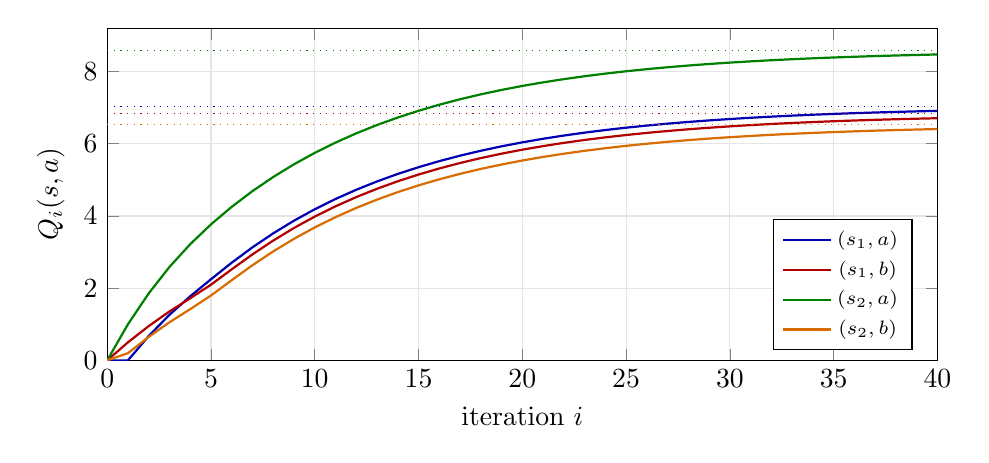
\begin{tikzpicture}
\begin{axis}[width=\linewidth, height=5.8cm, xmin=0, xmax=40, ymin=0, ymax=9.2, xlabel={iteration $i$}, ylabel={$Q_i(s,a)$}, grid=both, grid style={gray!20}, legend style={at={(0.97,0.03)}, anchor=south east, font=\scriptsize}]
\addplot[blue!70!black, thick] coordinates {(0.000000,0.000000) (1.000000,0.000000) (2.000000,0.675000) (3.000000,1.262250) (4.000000,1.774372) (5.000000,2.246689) (6.000000,2.705932) (7.000000,3.131547) (8.000000,3.519027) (9.000000,3.869353) (10.000000,4.185220) (11.000000,4.469707) (12.000000,4.725819) (13.000000,4.956347) (14.000000,5.163832) (15.000000,5.350572) (16.000000,5.518639) (17.000000,5.669900) (18.000000,5.806035) (19.000000,5.928556) (20.000000,6.038826) (21.000000,6.138068) (22.000000,6.227386) (23.000000,6.307773) (24.000000,6.380120) (25.000000,6.445233) (26.000000,6.503835) (27.000000,6.556577) (28.000000,6.604044) (29.000000,6.646764) (30.000000,6.685213) (31.000000,6.719817) (32.000000,6.750960) (33.000000,6.778989) (34.000000,6.804215) (35.000000,6.826919) (36.000000,6.847352) (37.000000,6.865742) (38.000000,6.882292) (39.000000,6.897188) (40.000000,6.910594)};
\addplot[red!70!black, thick] coordinates {(0.000000,0.000000) (1.000000,0.500000) (2.000000,0.950000) (3.000000,1.355000) (4.000000,1.719500) (5.000000,2.096935) (6.000000,2.522020) (7.000000,2.935339) (8.000000,3.318392) (9.000000,3.667124) (10.000000,3.982418) (11.000000,4.266698) (12.000000,4.522736) (13.000000,4.753237) (14.000000,4.960713) (15.000000,5.147449) (16.000000,5.315515) (17.000000,5.466775) (18.000000,5.602910) (19.000000,5.725431) (20.000000,5.835701) (21.000000,5.934943) (22.000000,6.024261) (23.000000,6.104648) (24.000000,6.176995) (25.000000,6.242108) (26.000000,6.300710) (27.000000,6.353452) (28.000000,6.400919) (29.000000,6.443639) (30.000000,6.482088) (31.000000,6.516692) (32.000000,6.547835) (33.000000,6.575864) (34.000000,6.601090) (35.000000,6.623794) (36.000000,6.644227) (37.000000,6.662617) (38.000000,6.679167) (39.000000,6.694063) (40.000000,6.707469)};
\addplot[green!50!black, thick] coordinates {(0.000000,0.000000) (1.000000,1.000000) (2.000000,1.855000) (3.000000,2.588050) (4.000000,3.218271) (5.000000,3.766493) (6.000000,4.253061) (7.000000,4.688513) (8.000000,5.079535) (9.000000,5.431136) (10.000000,5.747462) (11.000000,6.032114) (12.000000,6.288286) (13.000000,6.518835) (14.000000,6.726328) (15.000000,6.913070) (16.000000,7.081139) (17.000000,7.232400) (18.000000,7.368535) (19.000000,7.491056) (20.000000,7.601326) (21.000000,7.700568) (22.000000,7.789886) (23.000000,7.870273) (24.000000,7.942620) (25.000000,8.007733) (26.000000,8.066335) (27.000000,8.119077) (28.000000,8.166544) (29.000000,8.209264) (30.000000,8.247713) (31.000000,8.282317) (32.000000,8.313460) (33.000000,8.341489) (34.000000,8.366715) (35.000000,8.389419) (36.000000,8.409852) (37.000000,8.428242) (38.000000,8.444792) (39.000000,8.459688) (40.000000,8.473094)};
\addplot[orange!85!black, thick] coordinates {(0.000000,0.000000) (1.000000,0.200000) (2.000000,0.650000) (3.000000,1.055000) (4.000000,1.419500) (5.000000,1.796935) (6.000000,2.222020) (7.000000,2.635339) (8.000000,3.018392) (9.000000,3.367124) (10.000000,3.682418) (11.000000,3.966698) (12.000000,4.222736) (13.000000,4.453237) (14.000000,4.660713) (15.000000,4.847449) (16.000000,5.015515) (17.000000,5.166775) (18.000000,5.302910) (19.000000,5.425431) (20.000000,5.535701) (21.000000,5.634943) (22.000000,5.724261) (23.000000,5.804648) (24.000000,5.876995) (25.000000,5.942108) (26.000000,6.000710) (27.000000,6.053452) (28.000000,6.100919) (29.000000,6.143639) (30.000000,6.182088) (31.000000,6.216692) (32.000000,6.247835) (33.000000,6.275864) (34.000000,6.301090) (35.000000,6.323794) (36.000000,6.344227) (37.000000,6.362617) (38.000000,6.379167) (39.000000,6.394063) (40.000000,6.407469)};
\addplot[blue!70!black, dotted] coordinates {(0,7.03125)(40,7.03125)};
\addplot[red!70!black, dotted] coordinates {(0,6.828125)(40,6.828125)};
\addplot[green!50!black, dotted] coordinates {(0,8.59375)(40,8.59375)};
\addplot[orange!85!black, dotted] coordinates {(0,6.528125)(40,6.528125)};
\legend{{$(s_1,a)$},{$(s_1,b)$},{$(s_2,a)$},{$(s_2,b)$}}
\end{axis}
\end{tikzpicture}
\end{minipage}\hfill
\begin{minipage}{0.49\linewidth}
\centering
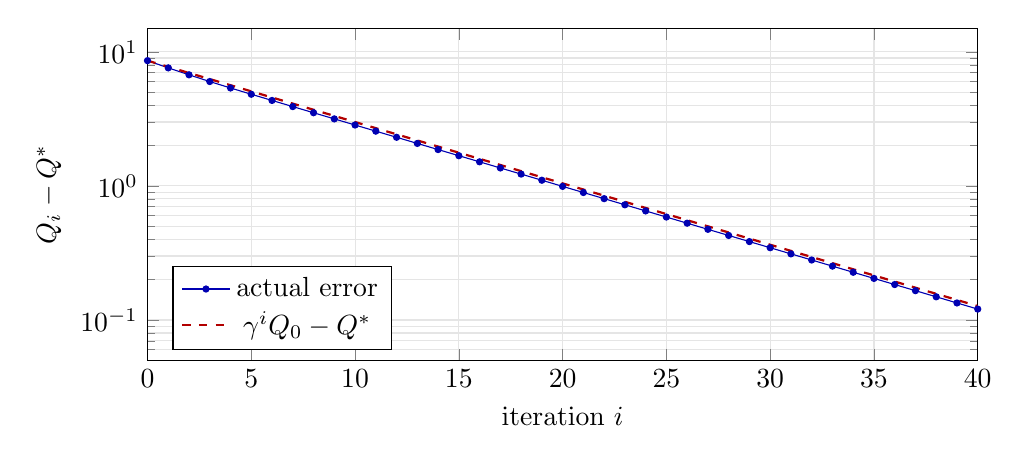
\begin{tikzpicture}
\begin{axis}[width=\linewidth, height=5.8cm, xmin=0, xmax=40, ymode=log, ymin=0.05, ymax=15, xlabel={iteration $i$}, ylabel={$\norm{Q_i-Q^*}$}, grid=both, grid style={gray!20}, legend pos=south west]
\addplot[blue!70!black, mark=*, mark size=1.1pt] coordinates {(0.000000,8.593750) (1.000000,7.593750) (2.000000,6.738750) (3.000000,6.005700) (4.000000,5.375479) (5.000000,4.827257) (6.000000,4.340689) (7.000000,3.905237) (8.000000,3.514215) (9.000000,3.162614) (10.000000,2.846288) (11.000000,2.561636) (12.000000,2.305464) (13.000000,2.074915) (14.000000,1.867422) (15.000000,1.680680) (16.000000,1.512611) (17.000000,1.361350) (18.000000,1.225215) (19.000000,1.102694) (20.000000,0.992424) (21.000000,0.893182) (22.000000,0.803864) (23.000000,0.723477) (24.000000,0.651130) (25.000000,0.586017) (26.000000,0.527415) (27.000000,0.474673) (28.000000,0.427206) (29.000000,0.384486) (30.000000,0.346037) (31.000000,0.311433) (32.000000,0.280290) (33.000000,0.252261) (34.000000,0.227035) (35.000000,0.204331) (36.000000,0.183898) (37.000000,0.165508) (38.000000,0.148958) (39.000000,0.134062) (40.000000,0.120656)};
\addplot[red!70!black, dashed, thick, domain=0:40, samples=41] {8.59375*0.9^x};
\legend{actual error, $\gamma^i\norm{Q_0-Q^*}$}
\end{axis}
\end{tikzpicture}
\end{minipage}
\caption{Value iteration on Example~\ref{ex:toy} ($\gamma=0.9$, $Q_0=0$), in the spirit of the demo on slide 52. Left: the four Q-values converge to $Q^*$ (dotted lines). Right: the error stays below the geometric bound of Theorem~\ref{thm:vi}.}
\label{fig:vi}
\end{figure}

\begin{example}[First iterations of value iteration]\label{ex:vi}
$Q_1=r$ (from $Q_0=0$). Then, e.g., $Q_2(s_1,a)=0+0.9\,(0.5\cdot\max Q_1(s_1,\cdot)+0.5\cdot\max Q_1(s_2,\cdot))=0.9(0.5\cdot0.5+0.5\cdot1)=0.675$, matching the table in Example~\ref{ex:greedy}. The fixed point is $Q^*=\begin{pmatrix}7.03125&6.828125\\8.59375&6.528125\end{pmatrix}$ (rows $s_1,s_2$; columns $a,b$), so $V^*=(7.03125,\,8.59375)$ and $\pi^*=(a,a)$.
\end{example}

%=====================================================================
\section{Policy from Value Iteration \slides{54--65}}\label{sec:greedy}
%=====================================================================
We know that $\pi^*(s)=\argmax_aQ^*(s,a)$, and since $Q_i(s,a)\approx Q^*(s,a)$ we can choose
\[
\pi_i(s)=\argmax_aQ_i(s,a).
\]
\textbf{What is the quality of such a policy?} For all states,

\pdfnum{8}
\begin{theorem}[Quality of the greedy policy]\label{thm:greedy}
Let $\pi_i(s)\in\argmax_aQ_i(s,a)$. Then for every state $s$,
\[
V^{\pi_i}(s)\;\ge\;V^*(s)-\frac{2\norm{Q_i-Q^*}}{1-\gamma}\;\ge\;V^*(s)-\frac{2\gamma^i\norm{Q_0-Q^*}}{1-\gamma}.
\]
\end{theorem}
\begin{proof}
Write $\varepsilon=\norm{Q_i-Q^*}$ and fix $s$. Using $V^{\pi_i}(s)=Q^{\pi_i}(s,\pi_i(s))$ and $V^*(s)=Q^*(s,\pi^*(s))$ (slide 56), add and subtract $Q^*(s,\pi_i(s))$ (slide 57):
\[
V^{\pi_i}(s)-V^*(s)=\underbrace{\big[Q^{\pi_i}(s,\pi_i(s))-Q^*(s,\pi_i(s))\big]}_{\text{(I)}}+\underbrace{\big[Q^*(s,\pi_i(s))-Q^*(s,\pi^*(s))\big]}_{\text{(II)}}.
\]
\emph{Term (I).} The two $Q$'s share the same reward term, which cancels (slide 58), so
\[
\text{(I)}=\gamma\,\E_{s'\sim p(\cdot\mid s,\pi_i(s))}\big[V^{\pi_i}(s')-V^*(s')\big].
\]
\emph{Term (II).} Insert $Q_i$ twice (slides 59--62):
\[
\text{(II)}=\underbrace{\big[Q^*(s,\pi_i(s))-Q_i(s,\pi_i(s))\big]}_{\ge-\varepsilon}+\underbrace{\big[Q_i(s,\pi_i(s))-Q_i(s,\pi^*(s))\big]}_{\ge0}+\underbrace{\big[Q_i(s,\pi^*(s))-Q^*(s,\pi^*(s))\big]}_{\ge-\varepsilon}\ \ge\ -2\varepsilon.
\]
The middle bracket is non-negative because $\pi_i$ maximises $Q_i$; the outer two are each at least $-\varepsilon$ by definition of $\varepsilon$.

\emph{Putting it together.} Let $\delta=\min_s\big[V^{\pi_i}(s)-V^*(s)\big]\le0$ (no policy beats $V^*$). Taking the state attaining the minimum, and bounding the expectation in (I) below by $\delta$,
\[
\delta\ge\gamma\delta-2\varepsilon\ \Longrightarrow\ \delta(1-\gamma)\ge-2\varepsilon\ \Longrightarrow\ \delta\ge-\frac{2\varepsilon}{1-\gamma}.
\]
This is the first inequality (it holds for every $s$ since $\delta$ is the minimum over $s$). The second inequality is Theorem~\ref{thm:vi}.
\end{proof}

\begin{remark}[The slides' ``repeat'' version, slides 63--65]
The slides stop at $V^{\pi_i}(s)-V^*(s)\ge\gamma\,\E_{s'}[V^{\pi_i}(s')-V^*(s')]-2\gamma^i\norm{Q_0-Q^*}$, using $\norm{Q_i-Q^*}\le\gamma^i\norm{Q_0-Q^*}$ twice, and then say ``repeat and get $1/(1-\gamma)$'': plugging the same bound into the expectation on the right again and again produces the geometric series $2\gamma^i\norm{Q_0-Q^*}\,(1+\gamma+\gamma^2+\cdots)=2\gamma^i\norm{Q_0-Q^*}/(1-\gamma)$. The $\delta$-trick above is the same argument written in one line.
\end{remark}

\begin{intuition}
\emph{Why a factor 2?} The greedy choice compares actions using $Q_i$ instead of $Q^*$; each of the two actions being compared (the one we pick and the true best) can be mis-valued by up to $\varepsilon$, in opposite directions, so the \emph{one-step} regret is up to $2\varepsilon$. \emph{Why $1/(1-\gamma)$?} A one-step mistake is not a one-time cost: the policy keeps following the same imperfect scores in all later states, so mistakes accumulate over the whole effective horizon. Note the guarantee is about the \emph{policy actually executed}, $V^{\pi_i}$, not about $Q_i$.
\end{intuition}

\begin{example}[The greedy policy on the two-state MDP]\label{ex:greedy}
Greedy policies $\pi_i=(\pi_i(s_1),\pi_i(s_2))$ from value iteration, with $\norm{Q_0-Q^*}=8.594$, so the bound of Theorem~\ref{thm:greedy} is $\tfrac{2\gamma^i}{1-\gamma}\cdot8.594=171.9\,\gamma^i$:
\begin{center}
\small
\begin{tabular}{@{}rcccccccc@{}}
\toprule
$i$ & $Q_i(s_1,a)$ & $Q_i(s_1,b)$ & $Q_i(s_2,a)$ & $Q_i(s_2,b)$ & $\norm{Q_i-Q^*}$ & $\pi_i$ & $\max_s(V^*-V^{\pi_i})$ & bound\\
\midrule
0 & 0.000 & 0.000 & 0.000 & 0.000 & 8.594 & (a,a) & 0.000 & 171.875 \\
1 & 0.000 & 0.500 & 1.000 & 0.200 & 7.594 & (b,a) & 2.031 & 154.688 \\
2 & 0.675 & 0.950 & 1.855 & 0.650 & 6.739 & (b,a) & 2.031 & 139.219 \\
3 & 1.262 & 1.355 & 2.588 & 1.055 & 6.006 & (b,a) & 2.031 & 125.297 \\
4 & 1.774 & 1.720 & 3.218 & 1.419 & 5.375 & (a,a) & 0.000 & 112.767 \\
5 & 2.247 & 2.097 & 3.766 & 1.797 & 4.827 & (a,a) & 0.000 & 101.490 \\
6 & 2.706 & 2.522 & 4.253 & 2.222 & 4.341 & (a,a) & 0.000 & 91.341 \\
8 & 3.519 & 3.318 & 5.080 & 3.018 & 3.514 & (a,a) & 0.000 & 73.987 \\
10 & 4.185 & 3.982 & 5.747 & 3.682 & 2.846 & (a,a) & 0.000 & 59.929 \\
15 & 5.351 & 5.147 & 6.913 & 4.847 & 1.681 & (a,a) & 0.000 & 35.388 \\
20 & 6.039 & 5.836 & 7.601 & 5.536 & 0.992 & (a,a) & 0.000 & 20.896 \\
30 & 6.685 & 6.482 & 8.248 & 6.182 & 0.346 & (a,a) & 0.000 & 7.286 \\
40 & 6.911 & 6.707 & 8.473 & 6.407 & 0.121 & (a,a) & 0.000 & 2.540 \\
\bottomrule
\end{tabular}
\end{center}
At $i=0$ all Q-values tie. For $i=1,2,3$ the greedy policy is $(b,a)$ and loses $2.031$ in $s_1$ (it takes the immediate reward $0.5$ of $b$ instead of the long-run better $a$); from $i=4$ on, it is $(a,a)=\pi^*$ with zero loss.
\end{example}

\begin{figure}[htbp]
\centering
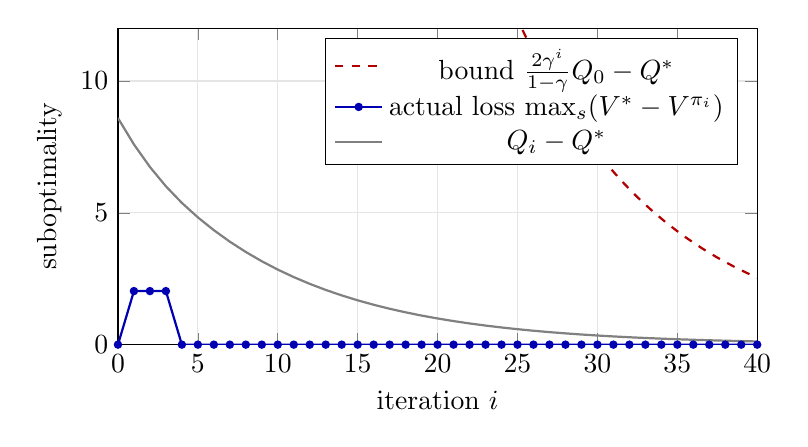
\begin{tikzpicture}
\begin{axis}[width=0.8\linewidth, height=5.6cm, xmin=0, xmax=40, ymin=0, ymax=12, xlabel={iteration $i$}, ylabel={suboptimality}, grid=both, grid style={gray!20}, legend pos=north east, clip=true]
\addplot[red!70!black, dashed, thick, domain=0:40, samples=81] {171.875*0.9^x};
\addplot[blue!70!black, thick, mark=*, mark size=1.1pt] coordinates {(0.000000,0.000000) (1.000000,2.031250) (2.000000,2.031250) (3.000000,2.031250) (4.000000,0.000000) (5.000000,0.000000) (6.000000,0.000000) (7.000000,0.000000) (8.000000,0.000000) (9.000000,0.000000) (10.000000,0.000000) (11.000000,0.000000) (12.000000,0.000000) (13.000000,0.000000) (14.000000,0.000000) (15.000000,0.000000) (16.000000,0.000000) (17.000000,0.000000) (18.000000,0.000000) (19.000000,0.000000) (20.000000,0.000000) (21.000000,0.000000) (22.000000,0.000000) (23.000000,0.000000) (24.000000,0.000000) (25.000000,0.000000) (26.000000,0.000000) (27.000000,0.000000) (28.000000,0.000000) (29.000000,0.000000) (30.000000,0.000000) (31.000000,0.000000) (32.000000,0.000000) (33.000000,0.000000) (34.000000,0.000000) (35.000000,0.000000) (36.000000,0.000000) (37.000000,0.000000) (38.000000,0.000000) (39.000000,0.000000) (40.000000,0.000000)};
\addplot[gray, thick] coordinates {(0.000000,8.593750) (1.000000,7.593750) (2.000000,6.738750) (3.000000,6.005700) (4.000000,5.375479) (5.000000,4.827257) (6.000000,4.340689) (7.000000,3.905237) (8.000000,3.514215) (9.000000,3.162614) (10.000000,2.846288) (11.000000,2.561636) (12.000000,2.305464) (13.000000,2.074915) (14.000000,1.867422) (15.000000,1.680680) (16.000000,1.512611) (17.000000,1.361350) (18.000000,1.225215) (19.000000,1.102694) (20.000000,0.992424) (21.000000,0.893182) (22.000000,0.803864) (23.000000,0.723477) (24.000000,0.651130) (25.000000,0.586017) (26.000000,0.527415) (27.000000,0.474673) (28.000000,0.427206) (29.000000,0.384486) (30.000000,0.346037) (31.000000,0.311433) (32.000000,0.280290) (33.000000,0.252261) (34.000000,0.227035) (35.000000,0.204331) (36.000000,0.183898) (37.000000,0.165508) (38.000000,0.148958) (39.000000,0.134062) (40.000000,0.120656)};
\legend{bound $\tfrac{2\gamma^i}{1-\gamma}\norm{Q_0-Q^*}$, actual loss $\max_s(V^*-V^{\pi_i})$, $\norm{Q_i-Q^*}$}
\end{axis}
\end{tikzpicture}
\caption{Guaranteed versus actual loss of the greedy policy (Example~\ref{ex:greedy}; original figure). The bound is vacuous (above the plotted range) until $i\approx26$, yet the greedy policy is already optimal from $i=4$. The theorem is a worst-case guarantee, not a prediction.}
\label{fig:greedy}
\end{figure}

%=====================================================================
\section{Number of Iterations of Value Iteration \slides{66--74}}\label{sec:iters}
%=====================================================================
\emph{Note: as with exact policy evaluation, the companion note lists this derivation as ``on the slides only''.}

If we want an $\epsilon$ error on the quality of the policy, we can determine the number of iterations $i$ by solving for it in
\[
\frac{2\gamma^i}{1-\gamma}\norm{Q_0-Q^*}\le\epsilon .
\]

\begin{proposition}[Number of iterations for an $\epsilon$-optimal greedy policy]\label{prop:iters}
Let $Q_0\in[0,1/(1-\gamma)]^{|\cS||\cA|}$ (e.g.\ $Q_0=0$) and rewards in $[0,1]$. If
\[
i\;\ge\;\frac{1}{1-\gamma}\,\ln\!\Big(\frac{2}{\epsilon(1-\gamma)^2}\Big),
\]
then $V^{\pi_i}(s)\ge V^*(s)-\epsilon$ for every state $s$.
\end{proposition}
\begin{proof}
\emph{Step 1 (slides 67--69).} $Q^*$ also lies in $[0,1/(1-\gamma)]$ (Fact~\ref{fact:range}), so by the infinity norm $\norm{Q_0-Q^*}\le1/(1-\gamma)$ (for $Q_0=0$ it is just $\norm{Q^*}\le1/(1-\gamma)$). Hence by Theorem~\ref{thm:greedy} it suffices that $\dfrac{2\gamma^i}{(1-\gamma)^2}\le\epsilon$.

\emph{Step 2 (slides 70--71).} Write $\gamma=1-(1-\gamma)$ (``add and subtract~1'') and use $1+x\le e^x$ for all real $x$ with $x=-(1-\gamma)$:
\[
\gamma^i=\big(1-(1-\gamma)\big)^i\le e^{-(1-\gamma)i}.
\]
So it suffices that $\dfrac{2e^{-(1-\gamma)i}}{(1-\gamma)^2}\le\epsilon$, i.e.\ $e^{-(1-\gamma)i}\le\dfrac{\epsilon(1-\gamma)^2}{2}$.

\emph{Step 3 (slides 72--74).} Take logarithms and use $\ln(1/x)=-\ln x$: $-(1-\gamma)i\le-\ln\!\big(\tfrac{2}{\epsilon(1-\gamma)^2}\big)$. Isolating $i$ gives the claimed condition.
\end{proof}

\begin{intuition}
\emph{Worked numbers} ($\epsilon=0.01$): for $\gamma=0.9$ the condition is $i\ge10\ln(20\,000)=99.03$, so \textbf{100 iterations}; for $\gamma=0.99$ it is $i\ge100\ln(2\cdot10^6)=1450.9$, so \textbf{1451 iterations}. Making $\gamma$ closer to one multiplies the work by about $10\times$ per extra ``nine'', while making $\epsilon$ ten times smaller adds only $\ln10/(1-\gamma)\approx23$ iterations at $\gamma=0.9$. In words: accuracy is cheap (logarithmic in $1/\epsilon$), the planning horizon $1/(1-\gamma)$ is what costs. Multiplying by the per-iteration cost, an $\epsilon$-optimal policy takes $O\big(|\cS|^2|\cA|\cdot\tfrac{1}{1-\gamma}\ln\tfrac1{\epsilon(1-\gamma)^2}\big)$ arithmetic operations. (Replacing $\ln(1/\gamma)$ by its lower bound $1-\gamma$ is a safe simplification: it can only make the required $i$ larger, e.g.\ $99.0$ instead of $94.0$ for $\gamma=0.9$.)
\end{intuition}

\begin{figure}[htbp]
\centering
\begin{tikzpicture}
\begin{axis}[width=0.8\linewidth, height=5.8cm, xmin=0.5, xmax=0.995, ymode=log, ymin=2, ymax=20000, xlabel={discount factor $\gamma$}, ylabel={iterations required}, grid=both, grid style={gray!20}, legend pos=north west]
\addplot[blue!70!black, thick, domain=0.5:0.995, samples=100] {ln(2/(0.1*(1-x)^2))/(1-x)};
\addplot[red!70!black, thick, domain=0.5:0.995, samples=100] {ln(2/(0.01*(1-x)^2))/(1-x)};
\addplot[gray, dashed, domain=0.5:0.995, samples=100] {1/(1-x)};
\legend{$\epsilon=0.1$, $\epsilon=0.01$, horizon $\tfrac{1}{1-\gamma}$}
\end{axis}
\end{tikzpicture}
\caption{Iterations sufficient for an $\epsilon$-optimal greedy policy (Proposition~\ref{prop:iters}; original figure, slides 66--74 only give the formula). The curves track the horizon $1/(1-\gamma)$ up to a logarithmic factor.}
\label{fig:iters}
\end{figure}

%=====================================================================
\section{Another Note on Value Iteration \slide{75}}
%=====================================================================
$Q_t$ is approximating $Q^*$, and from $Q_t$ we compute a policy $\pi_t$. \emph{However}, $Q_t$ is generally different from $Q^{\pi_t}$ until we converge to (approximately) $Q^*$. For example, $Q_0$ is just a random initial guess, which may not correspond to any policy's Q-value.

\begin{figure}[htbp]
\centering
\begin{tikzpicture}
\begin{axis}[width=0.8\linewidth, height=5.6cm, xmin=0, xmax=40, ymin=0, ymax=9, xlabel={iteration $i$}, ylabel={max-norm distance}, grid=both, grid style={gray!20}, legend pos=north east]
\addplot[gray, thick] coordinates {(0.000000,8.593750) (1.000000,7.593750) (2.000000,6.738750) (3.000000,6.005700) (4.000000,5.375479) (5.000000,4.827257) (6.000000,4.340689) (7.000000,3.905237) (8.000000,3.514215) (9.000000,3.162614) (10.000000,2.846288) (11.000000,2.561636) (12.000000,2.305464) (13.000000,2.074915) (14.000000,1.867422) (15.000000,1.680680) (16.000000,1.512611) (17.000000,1.361350) (18.000000,1.225215) (19.000000,1.102694) (20.000000,0.992424) (21.000000,0.893182) (22.000000,0.803864) (23.000000,0.723477) (24.000000,0.651130) (25.000000,0.586017) (26.000000,0.527415) (27.000000,0.474673) (28.000000,0.427206) (29.000000,0.384486) (30.000000,0.346037) (31.000000,0.311433) (32.000000,0.280290) (33.000000,0.252261) (34.000000,0.227035) (35.000000,0.204331) (36.000000,0.183898) (37.000000,0.165508) (38.000000,0.148958) (39.000000,0.134062) (40.000000,0.120656)};
\addplot[blue!70!black, thick, mark=*, mark size=1pt] coordinates {(0.000000,8.593750) (1.000000,6.631579) (2.000000,5.776579) (3.000000,5.043529) (4.000000,5.375479) (5.000000,4.827257) (6.000000,4.340689) (7.000000,3.905237) (8.000000,3.514215) (9.000000,3.162614) (10.000000,2.846288) (11.000000,2.561636) (12.000000,2.305464) (13.000000,2.074915) (14.000000,1.867422) (15.000000,1.680680) (16.000000,1.512611) (17.000000,1.361350) (18.000000,1.225215) (19.000000,1.102694) (20.000000,0.992424) (21.000000,0.893182) (22.000000,0.803864) (23.000000,0.723477) (24.000000,0.651130) (25.000000,0.586017) (26.000000,0.527415) (27.000000,0.474673) (28.000000,0.427206) (29.000000,0.384486) (30.000000,0.346037) (31.000000,0.311433) (32.000000,0.280290) (33.000000,0.252261) (34.000000,0.227035) (35.000000,0.204331) (36.000000,0.183898) (37.000000,0.165508) (38.000000,0.148958) (39.000000,0.134062) (40.000000,0.120656)};
\addplot[red!70!black, thick, dashed] coordinates {(0,1.828125) (1,1.828125) (2,1.828125) (3,1.828125) (4,0.000000) (5,0.000000) (6,0.000000) (7,0.000000) (8,0.000000) (9,0.000000) (10,0.000000) (11,0.000000) (12,0.000000) (13,0.000000) (14,0.000000) (15,0.000000) (16,0.000000) (17,0.000000) (18,0.000000) (19,0.000000) (20,0.000000) (21,0.000000) (22,0.000000) (23,0.000000) (24,0.000000) (25,0.000000) (26,0.000000) (27,0.000000) (28,0.000000) (29,0.000000) (30,0.000000) (31,0.000000) (32,0.000000) (33,0.000000) (34,0.000000) (35,0.000000) (36,0.000000) (37,0.000000) (38,0.000000) (39,0.000000) (40,0.000000)};
\legend{$\norm{Q_i-Q^*}$, $\norm{Q_i-Q^{\pi_i}}$, $\norm{Q^{\pi_i}-Q^*}$}
\end{axis}
\end{tikzpicture}
\caption{On Example~\ref{ex:toy}: the iterate $Q_i$ is far from the Q-function $Q^{\pi_i}$ of its own greedy policy for many iterations, even after $\pi_i$ has become optimal ($i\ge4$, where $\norm{Q^{\pi_i}-Q^*}=0$). Ties at $i=0$ are broken towards $a$. (Original figure; slide 75 is text only.)}
\label{fig:qpi}
\end{figure}

\begin{intuition}
Value iteration is \emph{not} ``evaluate a policy, then improve it''. The intermediate tables $Q_i$ are only approximations of $Q^*$; there may not exist any policy whose Q-function equals $Q_i$. In the two-state MDP, $Q_1=r$, but every policy has strictly positive values, so $Q^\pi(s,a)=r(s,a)+\gamma\E V^\pi(s')>r(s,a)$ for all $\pi$: $Q_1$ is the Q-function of \emph{no} policy. Only in the limit does $Q_i$ become $Q^*=Q^{\pi^*}$. This is why Theorem~\ref{thm:greedy} is needed at all: it tells us what the greedy policy of an imperfect $Q_i$ is worth.
\end{intuition}
%=====================================================================
\section{Summary}
%=====================================================================
\subsection{Comparison of the methods and results}
\begin{center}
\small
\renewcommand{\arraystretch}{1.25}
\begin{tabular}{@{}>{\raggedright\arraybackslash}p{2.5cm}>{\raggedright\arraybackslash}p{2.9cm}>{\raggedright\arraybackslash}p{3.7cm}>{\raggedright\arraybackslash}p{4.9cm}c@{}}
\toprule
\textbf{Method} & \textbf{Computes / operator} & \textbf{Cost} & \textbf{Guarantee} & \textbf{Slides}\\
\midrule
Exact policy evaluation & $V^\pi$; solve $(I-\gamma P^\pi)V=r^\pi$ & $O(|\cS|^3)$ & exact (Prop.~\ref{prop:exact}) & 16--22\\
Iterative policy evaluation & $V^\pi$; $\Bpi$ (affine, $\gamma$-contraction) & $O(|\cS|^2)$ per sweep; $O(|\cS|^2\ln\frac1\epsilon)$ in total & $\norm{V_i-V^\pi}\le\gamma^i\norm{V_0-V^\pi}$ (Cor.~\ref{cor:pe}) & 29--38\\
Naive policy search & $\pi^*$; evaluate every policy & $O(|\cA|^{|\cS|}|\cS|^3)$ & exact, but exponential & 39--42\\
Value iteration & $Q^*$; $\Bell$ (non-linear, $\gamma$-contraction) & $O(|\cS|^2|\cA|)$ per iteration & $\norm{Q_i-Q^*}\le\gamma^i\norm{Q_0-Q^*}$ (Thm.~\ref{thm:vi}) & 49--53\\
Greedy policy from VI & $\pi_i=\argmax_aQ_i$ & free (an $\argmax$) & $V^{\pi_i}\ge V^*-\frac{2\gamma^i}{1-\gamma}\norm{Q_0-Q^*}$ (Thm.~\ref{thm:greedy}) & 54--65\\
$\epsilon$-optimal policy & number of iterations & $i\ge\frac1{1-\gamma}\ln\frac{2}{\epsilon(1-\gamma)^2}$ & $V^{\pi_i}\ge V^*-\epsilon$ (Prop.~\ref{prop:iters}) & 66--74\\
\bottomrule
\end{tabular}
\end{center}

\subsection{Cost scaling}
\begin{figure}[htbp]
\centering
\begin{tikzpicture}
\begin{axis}[width=0.85\linewidth, height=6.2cm, xmin=2, xmax=30, ymode=log, ymin=1, ymax=1e15, xlabel={number of states $|\cS|$ (with $|\cA|=2$)}, ylabel={arithmetic operations (order of magnitude)}, grid=both, grid style={gray!20}, legend style={at={(0.03,0.97)}, anchor=north west, font=\scriptsize}]
\addplot[red!70!black, very thick, domain=2:30, samples=60] {2^x*x^3};
\addplot[black!60, thick, dashed, domain=2:30, samples=60] {x^3};
\addplot[blue!70!black, thick, domain=2:30, samples=60] {65*x^2};
\addplot[green!50!black, very thick, domain=2:30, samples=60] {200*x^2};
\legend{{naive policy search $|\cA|^{|\cS|}|\cS|^3$},{one exact evaluation $|\cS|^3$},{iterative evaluation ($\epsilon{=}0.01$, $\gamma{=}0.9$)},{value iteration for $\epsilon$-optimal policy}}
\end{axis}
\end{tikzpicture}
\caption{Qualitative cost comparison (original figure; constants dropped, iteration counts from the worked examples: $65$ sweeps for evaluation, $100$ iterations $\times\,|\cA|=2$ for value iteration, $\gamma=0.9$, $\epsilon=0.01$). Enumerating policies explodes exponentially; value iteration stays polynomial.}
\label{fig:costs}
\end{figure}

\subsection{Key take-aways}
\begin{itemize}
  \item \textbf{Policy evaluation is a linear problem.} $V^\pi=(I-\gamma P^\pi)^{-1}r^\pi$ exactly in $O(|\cS|^3)$, or approximately by iterating $V_{i+1}=r^\pi+\gamma P^\pi V_i$ at $O(|\cS|^2)$ per sweep and $O(\ln\frac1\epsilon)$ sweeps.
  \item \textbf{Contractions are the engine.} A $k$-contraction on a complete metric space has a unique fixed point and fixed-point iteration converges to it at rate $k^i$ (Banach). Both $\Bpi$ and $\Bell$ are $\gamma$-contractions in the sup-norm, because rewards cancel and averages cannot exceed maxima; hence $V^\pi$, $V^*$ and $Q^*$ are their unique fixed points.
  \item \textbf{Value iteration} $Q_{i+1}=\Bell Q_i$ converges geometrically, $\norm{Q_i-Q^*}\le\gamma^i\norm{Q_0-Q^*}$, at $O(|\cS|^2|\cA|)$ per iteration, avoiding the $|\cA|^{|\cS|}$ policy enumeration.
  \item \textbf{The greedy policy is near-optimal, with a $\frac{2}{1-\gamma}$ penalty:} $V^{\pi_i}\ge V^*-\frac{2\gamma^i}{1-\gamma}\norm{Q_0-Q^*}$, so $i\ge\frac1{1-\gamma}\ln\frac2{\epsilon(1-\gamma)^2}$ iterations give an $\epsilon$-optimal policy: accuracy is logarithmic, the horizon $\frac1{1-\gamma}$ is what costs.
  \item \textbf{The intermediate $Q_i$ are not policy values.} Value iteration does not alternate evaluation and improvement; $Q_i$ is generally different from $Q^{\pi_i}$ until convergence, and the bound in Theorem~\ref{thm:greedy} is a worst-case guarantee that is often very pessimistic (\figref{fig:greedy}).
\end{itemize}

%=====================================================================
\appendix
\section{Supplementary: Banach's Theorem, Existence and Rate}\label{app:banach}
%=====================================================================
\emph{This appendix is \textbf{not covered on the slides}; it comes from the companion note only. The slides state the uniqueness half of Theorem~\ref{thm:banach} (slide 25) and then use convergence of fixed-point iteration (slides 23--24, 29--38, 49--53) without proving it.}

\begin{proof}[Proof of Theorem~\ref{thm:banach}: existence and rate]
\emph{Existence.} From $x_{i+1}=f(x_i)$ we get $d(x_{i+1},x_i)=d(f(x_i),f(x_{i-1}))\le k\,d(x_i,x_{i-1})$, hence $d(x_{i+1},x_i)\le k^i\,d(x_1,x_0)$ by induction. For $j>i$ the triangle inequality gives
\[
d(x_j,x_i)\le\sum_{l=i}^{j-1}d(x_{l+1},x_l)\le\sum_{l=i}^{j-1}k^l\,d(x_1,x_0)\le\frac{k^i}{1-k}\,d(x_1,x_0),
\]
which tends to $0$ as $i\to\infty$: the sequence is Cauchy, and by completeness it has a limit $x^*$. A contraction is continuous (it is Lipschitz), so $f(x^*)=f(\lim x_i)=\lim f(x_i)=\lim x_{i+1}=x^*$.

\emph{Rate.} Since $f(x^*)=x^*$, $d(x_i,x^*)=d(f(x_{i-1}),f(x^*))\le k\,d(x_{i-1},x^*)$, and induction gives $d(x_i,x^*)\le k^i\,d(x_0,x^*)$.
\end{proof}

\begin{intuition}
The sequence of iterates is a walk whose steps shrink geometrically ($d(x_{i+1},x_i)\le k^id(x_1,x_0)$), so the \emph{total remaining path length} is a convergent geometric series. A walk with summable steps cannot wander forever: it settles somewhere (completeness says that ``somewhere'' is a point of the space), and by continuity that limit must be unmoved by $f$. The rate is then just the contraction inequality applied to the pair $(x_{i-1},x^*)$.
\end{intuition}

%=====================================================================
\section{Supplementary: Self-Check List from the Companion Note}\label{app:selfcheck}
%=====================================================================
\emph{Study aid reproduced from the companion note (not a slide topic). ``State'' means: write the statement with assumptions and say in one sentence what it claims (for an algorithm: write its steps). ``Prove'' means: write the proof without looking. The last column gives the proof video of the same lecture on Classroom and where the item lives in these notes.}

\begin{center}
\small
\renewcommand{\arraystretch}{1.2}
\begin{tabular}{@{}>{\raggedright\arraybackslash}p{6.0cm}cc>{\raggedright\arraybackslash}p{4.9cm}@{}}
\toprule
\textbf{Item} & \textbf{state} & \textbf{prove} & \textbf{Video / location here}\\
\midrule
On the slides only: exact policy evaluation (slides 16--22) & $\square$ & $\square$ & Prop.~\ref{prop:exact}, \S\ref{sec:exact}\\
Definition 1 (contraction) & $\square$ & & \S\ref{sec:contr}\\
Theorem 2 (Banach) & $\square$ & $\square$ & \texttt{ch05-banach.mp4}; \S\ref{sec:contr}, App.~\ref{app:banach}\\
Definition 3 (Bellman operators) & $\square$ & & \S\ref{sec:itpe}\\
Theorem 4 (both $\gamma$-contractions) & $\square$ & $\square$ & \texttt{ch05-contraction.mp4}; \S\ref{sec:thm4}, \S\ref{sec:optcontr}\\
Corollary 5 (what the fixed points are) & $\square$ & $\square$ & \texttt{ch05-vi.mp4}; \S\ref{sec:vi}\\
Algorithm A (iterative policy evaluation) & $\square$ & & \S\ref{sec:itpe}\\
Corollary 6 (convergence and cost) & $\square$ & $\square$ & \texttt{ch05-vi.mp4}; \S\ref{sec:peiters}\\
Algorithm B (value iteration) & $\square$ & & \S\ref{sec:vi}\\
Theorem 7 (VI converges geometrically) & $\square$ & $\square$ & \texttt{ch05-vi.mp4}; \S\ref{sec:vi}\\
Theorem 8 (quality of the greedy policy) & $\square$ & $\square$ & \texttt{ch05-greedyquality.mp4}; \S\ref{sec:greedy}\\
On the slides only: iterations of VI for an $\epsilon$-optimal policy (slides 66--74) & $\square$ & $\square$ & Prop.~\ref{prop:iters}, \S\ref{sec:iters}\\
\bottomrule
\end{tabular}
\end{center}

\newpage

% ======================================================================
% Lecture 3 -- Part 2
% ======================================================================
\part{Lecture 3 -- Part 2}

\section*{Setting, notation and imported results}
\addcontentsline{toc}{section}{Setting, notation and imported results}

Throughout, $(\Sset,\Aset,p,r,\gamma)$ is a finite discounted MDP with $\gamma\in[0,1)$, transition kernel $p(s'\mid s,a)$ and rewards $r(s,a)\in[0,1]$. A policy $\pi(a\mid s)$ may be stochastic; deterministic stationary policies are the special case in which $\pi(\cdot\mid s)$ is a point mass, written $\pi(s)$. The value functions are
\[
V^\pi(s)=\E^\pi\Big[\sum_{t\ge 0}\gamma^t r(s_t,a_t)\,\Big|\,s_0=s\Big],\qquad
Q^\pi(s,a)=r(s,a)+\gamma\,\E_{s'\sim p(\cdot\mid s,a)}\big[V^\pi(s')\big],
\]
so that $V^\pi(s)=\E_{a\sim\pi(\cdot|s)}Q^\pi(s,a)$ and, because $r\in[0,1]$, $0\le Q^\pi,V^\pi\le 1/(1-\gamma)$. In vector form (functions on $\Sset$ are vectors in $\R^{|\Sset|}$) let
\[
r^\pi(s)=\sum_a\pi(a\mid s)\,r(s,a),\qquad P^\pi(s,s')=\sum_a\pi(a\mid s)\,p(s'\mid s,a),
\]
so $P^\pi$ is a row-stochastic matrix. Two operators on value functions will be used:
\[
(B^\pi V)=r^\pi+\gamma P^\pi V,\qquad (\B V)(s)=\max_a\Big\{r(s,a)+\gamma\,\E_{s'\sim p(\cdot|s,a)}V(s')\Big\}.
\]
The sup-norm is $\norm{\cdot}$. Inequalities between functions hold pointwise.

\paragraph{Results imported from earlier lectures} (used, not re-proved here).
\begin{center}\small
\begin{tabular}{@{}lp{0.74\textwidth}@{}}
\toprule
\textbf{Label} & \textbf{Content as used below}\\
\midrule
L03, Lemma 3 & Value functions and discounted sums are bounded (by $1/(1-\gamma)$ here), so all series below converge absolutely.\\
L03, Lemma 5 & A discounted sum along trajectories equals $\frac1{1-\gamma}$ times an expectation under the discounted occupancy measure (defined in Section~\ref{sec:pdl}).\\
L03, Theorem 6 & Bellman expectation equations: $Q^\pi(s,a)=r(s,a)+\gamma\E_{s'}V^\pi(s')$ and $V^\pi=B^\pi V^\pi$.\\
L03, Theorem 8 & The optimal value function satisfies $\B V^*=V^*$.\\
L03, Theorem 10 & Any fixed point of $\B$ is $V^*$.\\
L04, Theorem 2 & Value iteration converges: $\B^kV\to V^*$ for every bounded $V$.\\
L04, Theorem 4 & $\B$ is a $\gamma$-contraction in sup-norm: $\norm{\B U-\B V}\le\gamma\norm{U-V}$.\\
\bottomrule
\end{tabular}
\end{center}

%=====================================================================
\section{Recap\sltag{2--11}}
%=====================================================================
Policy iteration is built from two ingredients seen earlier: \emph{evaluating} a fixed policy and \emph{improving} it. This section collects exactly what is needed.

%---------------------------------------------------------------------
\subsection{Bellman Equation\sltag{3}}
The value of a state is the current reward plus the discounted value of where we land next, with the next state drawn according to the policy.

\begin{theorem}[Bellman expectation equations]\label{thm:bellman-exp}
For every policy $\pi$,
\[
V^\pi(s)=r(s,\pi(s))+\gamma\,\E_{s'\sim p(\cdot\mid s,\pi(s))}\big[V^\pi(s')\big],\qquad
Q^\pi(s,a)=r(s,a)+\gamma\,\E_{s'\sim p(\cdot\mid s,a)}\big[V^\pi(s')\big],
\]
and consequently $V^\pi(s)=Q^\pi(s,\pi(s))$ (for deterministic $\pi$; in general $V^\pi(s)=\E_{a\sim\pi}Q^\pi(s,a)$).
\end{theorem}

\begin{intuition}
In $V^\pi(s)$ the action is dictated by $\pi$; in $Q^\pi(s,a)$ the \emph{first} action $a$ is forced and only afterwards does $\pi$ take over. Both share the same one-step structure: ``reward now + $\gamma\times$ value of the next state''. The only difference is who picks the first action. This one-step view is what lets us compare policies by changing a single decision.
\end{intuition}

%---------------------------------------------------------------------
\subsection{Bellman Optimality Example\sltag{4}}
Take a state $s$ with two actions $a'$ and $a''$ leading to $s'$ and $s''$, and assume $V^*$ is known at the successors. Trying each action gives $Q^*(s,a')=r(s,a')+\gamma V^*(s')$ and $Q^*(s,a'')=r(s,a'')+\gamma V^*(s'')$, and
\[
V^*(s)=\max_a\Big[r(s,a)+\gamma\,\E_{s'\sim p(\cdot|s,a)}V^*(s')\Big]=\max\big\{Q^*(s,a'),\,Q^*(s,a'')\big\}.
\]

\begin{figure}[h]
\centering
\begin{tikzpicture}[st/.style={circle,draw,fill=green!25,minimum size=9mm,inner sep=0pt}]
\node[st] (s) at (0,1.9) {$s$};
\node[st] (s1) at (-2.2,0) {$s'$};
\node[st] (s2) at (2.2,0) {$s''$};
\draw[-{Latex}] (s)--node[left=3pt]{$a'$}(s1);
\draw[-{Latex}] (s)--node[right=3pt]{$a''$}(s2);
\node[below=1pt of s1,font=\small] {$V^*(s')$ known};
\node[below=1pt of s2,font=\small] {$V^*(s'')$ known};
\node[right=10pt of s,font=\small,align=left,text width=5.2cm] {$Q^*(s,a')=r(s,a')+\gamma V^*(s')$\\[2pt]$Q^*(s,a'')=r(s,a'')+\gamma V^*(s'')$\\[2pt]$V^*(s)=\max\{Q^*(s,a'),Q^*(s,a'')\}$};
\end{tikzpicture}
\caption{One-step lookahead behind the Bellman optimality equation (redrawn).}
\end{figure}

\begin{intuition}
\emph{Worked numbers} ($\gamma=0.9$, deterministic moves): if $r(s,a')=1$ and $V^*(s')=10$, then $Q^*(s,a')=1+9=10$; if $r(s,a'')=0$ and $V^*(s'')=12$, then $Q^*(s,a'')=10.8$. So $V^*(s)=10.8$ and the best action is $a''$ even though its immediate reward is smaller: a good destination can outweigh a good first reward.
\end{intuition}

%---------------------------------------------------------------------
\subsection{Exact Policy Evaluation\sltag{5}}
The Bellman equation holds for \emph{all} states at once, so the $|\Sset|$ scalar equations stack into one linear system
\[
V^\pi=r^\pi+\gamma P^\pi V^\pi\quad\Longleftrightarrow\quad (I-\gamma P^\pi)V^\pi=r^\pi\quad\Longleftrightarrow\quad V^\pi=(I-\gamma P^\pi)^{-1}r^\pi .
\]

\begin{lemma}\label{lem:inv}
$I-\gamma P^\pi$ is invertible and $(I-\gamma P^\pi)^{-1}=\sum_{k\ge0}\gamma^k(P^\pi)^k$.
\end{lemma}
\begin{proof}
$P^\pi$ is row-stochastic, so $\norm{P^\pi}=1$ in the induced norm and $\norm{\gamma P^\pi}=\gamma<1$. The Neumann series converges, and multiplying it by $I-\gamma P^\pi$ telescopes to $I$.
\end{proof}

\begin{figure}[h]
\centering
\begin{tikzpicture}[x=1cm,y=1cm,every node/.style={font=\small}]
\def\rowsfor#1#2#3{\foreach \i in {1,...,5}{\draw[gray!60] (#1,\i*0.5) -- (#2,\i*0.5);}}
% V
\draw (0,0) rectangle (0.6,3); \node at (0.3,3.35) {$V^\pi$};
\rowsfor{0}{0.6}{}
\fill[red!25] (0,1.5) rectangle (0.6,2); \node at (0.3,1.75) {\scriptsize $s$};
\node at (1.05,1.5) {$=$};
% r
\draw (1.5,0) rectangle (3.3,3); \node at (2.4,3.35) {$r^\pi$};
\rowsfor{1.5}{3.3}{}
\fill[red!25] (1.5,1.5) rectangle (3.3,2); \node at (2.4,1.75) {\scriptsize $r(s,\pi(s))$};
\node at (3.85,1.5) {$+\ \gamma$};
% P
\draw (4.5,0) rectangle (7.5,3); \node at (6.0,3.35) {$P^\pi$};
\rowsfor{4.5}{7.5}{}
\fill[red!25] (4.5,1.5) rectangle (7.5,2); \node at (6.0,1.75) {\scriptsize $p(s'\mid s,\pi(s))$};
% V
\draw (7.9,0) rectangle (8.5,3); \node at (8.2,3.35) {$V^\pi$};
\rowsfor{7.9}{8.5}{}
\end{tikzpicture}
\caption{Stacking the Bellman equations: row $s$ of the matrix product is exactly the scalar equation for state $s$.}
\end{figure}

\begin{intuition}
It is a ``nice but expensive'' fix: one linear solve gives the exact value of a policy, but inverting (or factorising) a $|\Sset|\times|\Sset|$ matrix costs $O(|\Sset|^3)$. This is the price paid for exactness, and it dominates the cost of each policy iteration step later on.
\end{intuition}

%---------------------------------------------------------------------
\subsection{Fixed-Point Iteration \& Contractions\sltag{6}}
A \emph{fixed point} of $f$ is a point with $x=f(x)$. To find one: initialise $x_0$, repeat $x_{k+1}=f(x_k)$, and stop when $x$ no longer changes.

\begin{definition}[Contraction mapping]
A map $f:M\to M$ on a metric space $(M,d)$ is a contraction if $d(f(x),f(x'))\le \kappa\, d(x,x')$ for some $\kappa\in[0,1)$ and all $x,x'$.
\end{definition}

\begin{theorem}[Banach fixed-point theorem (standard)]\label{thm:banach}
If $(M,d)$ is complete and $f$ is a $\kappa$-contraction, then $f$ has a unique fixed point $x^\star$ and, for every $x_0$, $d(x_k,x^\star)\le\kappa^k d(x_0,x^\star)$.
\end{theorem}
\begin{proof}
Uniqueness: two fixed points $x,x'$ satisfy $d(x,x')=d(fx,fx')\le\kappa d(x,x')$, forcing $d(x,x')=0$. Existence: $d(x_{k+1},x_k)\le\kappa^k d(x_1,x_0)$, so $(x_k)$ is Cauchy (geometric tails), and its limit $x^\star$ is a fixed point by continuity of $f$. Finally $d(x_k,x^\star)=d(fx_{k-1},fx^\star)\le\kappa\,d(x_{k-1},x^\star)$; iterate.
\end{proof}

\begin{figure}[h]
\centering
\begin{tikzpicture}
\begin{axis}[width=0.62\textwidth,height=6cm,xmin=0,xmax=8,ymin=0,ymax=8,axis lines=left,
 xlabel={$x$},ylabel={},legend pos=south east,legend style={font=\small},xtick={1,5},xticklabels={$x_0$,$x^\star$},ytick=\empty,clip=false]
\addplot[domain=0:8,thick,blue!70!black]{0.6*x+2};
\addplot[domain=0:8,dashed,gray]{x};
\addplot[red!70!black,thick,-{Latex}] coordinates {(1.0000,0.0000) (1.0000,2.6000) (2.6000,2.6000) (2.6000,3.5600) (3.5600,3.5600) (3.5600,4.1360) (4.1360,4.1360) (4.1360,4.4816) (4.4816,4.4816) (4.4816,4.6890) (4.6890,4.6890) (4.6890,4.8134) (4.8134,4.8134) (4.8134,4.8880) (4.8880,4.8880)};
\legend{$y=f(x)$,$y=x$,iterates}
\end{axis}
\end{tikzpicture}
\caption{Cobweb view of fixed-point iteration for the contraction $f(x)=0.6x+2$ (original illustration): each step jumps vertically to the graph, then horizontally to the diagonal, and spirals into $x^\star=5$.}
\end{figure}

\begin{intuition}
A contraction pulls any two points closer by a constant factor at every application, so repeated application squeezes everything onto a single point, no matter where we start. Every method below (iterative policy evaluation, value iteration) is ``apply a contraction until it stops moving''.
\end{intuition}

%---------------------------------------------------------------------
\subsection{Iterative Policy Evaluation\sltag{7}}
To avoid the cubic cost, initialise $V_0\in[0,1/(1-\gamma)]$ (typically $0$) and iterate, in matrix form because all states are updated at once,
\[
V_{i+1}=r^\pi+\gamma P^\pi V_i\qquad\text{until convergence.}
\]
\begin{lemma}\label{lem:Bpi}
$B^\pi$ is a $\gamma$-contraction in sup-norm with fixed point $V^\pi$; hence $\norm{V_{i+1}-V^\pi}\le\gamma\norm{V_i-V^\pi}\le\gamma^{i+1}\norm{V_0-V^\pi}$.
\end{lemma}
\begin{proof}
$B^\pi U-B^\pi V=\gamma P^\pi(U-V)$ and each row of $P^\pi$ is a probability vector, so $\norm{P^\pi(U-V)}\le\norm{U-V}$. Theorem~\ref{thm:banach} gives the rate, and $V^\pi=B^\pi V^\pi$ by Theorem~\ref{thm:bellman-exp}.
\end{proof}

\begin{intuition}
Each sweep costs only $O(|\Sset|^2)$ (one matrix--vector product) and the error shrinks by $\gamma$ per sweep. With $\gamma=0.9$ the error falls below $1\%$ of its start after about $44$ sweeps. A discount close to $1$ makes the future matter more and the iteration slower.
\end{intuition}

%---------------------------------------------------------------------
\subsection{How to Find the Optimal Policy?\sltag{8}}
What we really want is $\pi^*$. For that use Bellman \emph{optimality} and its operator, which acts on action-value functions $Q:\Sset\times\Aset\to\R$ and returns another such function:
\[
\B Q(s,a)=r(s,a)+\gamma\,\E_{s'\sim p(\cdot\mid s,a)}\Big[\max_{a'}Q(s',a')\Big].
\]
This operator is a $\gamma$-contraction in sup-norm (L04, Theorem 4), with $Q^*$ as unique fixed point.

%---------------------------------------------------------------------
\subsection{Value Iteration \& Optimal Policy\sltag{9}}
Since $Q^*=\B Q^*$, initialise $\norm{Q_0}\le1/(1-\gamma)$ (typically $Q_0=0$) and iterate, for all states and actions, $Q_{i+1}=\B Q_i$. Then
\[
\norm{Q_{i+1}-Q^*}=\norm{\B Q_i-\B Q^*}\le\gamma\norm{Q_i-Q^*}\le\gamma^{i+1}\norm{Q_0-Q^*}.
\]
Because $\pi^*(s)=\argmax_aQ^*(s,a)$ and $Q_i\approx Q^*$, we read off the policy $\pi_i(s)=\argmax_aQ_i(s,a)$.

%---------------------------------------------------------------------
\subsection{Another Note on Value Iteration\sltag{10}}
$Q_t$ approximates $Q^*$ and the policy $\pi_t$ is computed from $Q_t$. However, $Q_t$ is in general \emph{different from} $Q^{\pi_t}$ until we are close to $Q^*$: for instance $Q_0$ is just an initial guess, which may correspond to no policy at all.

\begin{intuition}
Value iteration outputs numbers that need not be the value of anything real. Concretely, since $Q^\pi(s,a)\ge r(s,a)$ for every $\pi$, the all-zero guess $Q_0\equiv0$ is the $Q$-function of no policy as soon as one reward is positive. Policy iteration, introduced next, fixes this: its intermediate objects \emph{are} values of actual policies.
\end{intuition}

%=====================================================================
\section{Policy Iteration\sltag{12--20}}
%=====================================================================
Policy iteration (PI) outputs a \emph{policy} at every iteration, $\{\pi_0,\pi_1,\dots,\pi_T\}$, whereas value iteration outputs value estimates. We start from an arbitrary guess $\pi_0$ (deterministic or stochastic) and alternate two steps. For simplicity, and to forget about approximation errors, the evaluation is assumed exact.

\begin{algo}[Policy iteration]\label{alg:pi}
Start from any policy $\pi_0$. For $t=0,1,2,\dots$:
\begin{enumerate}[leftmargin=2.2em,itemsep=2pt]
\item \textbf{Policy evaluation.} Compute $Q^{\pi_t}(s,a)$ for all $s,a$, e.g. $V^{\pi_t}=(I-\gamma P^{\pi_t})^{-1}r^{\pi_t}$ and then $Q^{\pi_t}(s,a)=r(s,a)+\gamma\E_{s'}[V^{\pi_t}(s')]$.
\item \textbf{Policy improvement.} $\pi_{t+1}(s)\in\argmax_aQ^{\pi_t}(s,a)$ for every $s$, \emph{keeping $\pi_t(s)$ whenever it is among the maximisers}.
\end{enumerate}
Stop when $\pi_{t+1}=\pi_t$.
\end{algo}

The slides' reminder $Q^\pi(s_t,a)=r_t+\gamma\E_{s'\sim p(\cdot|s,a)}[V^\pi(s')]$ explains the remark in step 1: it is convenient to compute $V$ first and obtain $Q$ from it. Unlike value iteration, the quantity produced is the $Q$-function of an actual policy.

\begin{intuition}
The tie-breaking clause in step 2 is not an implementation detail. If two actions have equal value, an arbitrary choice may swap them back and forth forever, producing policies that are worth the same (take one state with two actions, both with the same reward and a self-loop: every swap is allowed, none helps). Keeping the current action whenever it is a maximiser guarantees that any change of policy is a \emph{strict} improvement somewhere, which is what termination (Section~\ref{sec:terminate}) relies on.
\end{intuition}

\begin{example}[A two-state MDP, solved by hand]\label{ex:two}
States $A,B$ with actions \emph{stay} and \emph{go}, deterministic moves, $\gamma=0.9$. Staying in $A$ gives reward $0.5$, staying in $B$ gives reward $1$; \emph{go} gives reward $0$ and switches state.
\begin{center}\small
\begin{tabular}{@{}lcccc@{}}\toprule
 & $V^{\pi_t}(A)$ & $V^{\pi_t}(B)$ & $Q^{\pi_t}$ at $A$ (stay, go) & $Q^{\pi_t}$ at $B$ (stay, go)\\\midrule
$\pi_0=(\text{stay},\text{stay})$ & $5$ & $10$ & $(5,\ \mathbf{9})$ & $(\mathbf{10},\ 4.5)$\\
$\pi_1=(\text{go},\text{stay})$ & $9$ & $10$ & $(8.6,\ \mathbf{9})$ & $(\mathbf{10},\ 8.1)$\\\bottomrule
\end{tabular}
\end{center}
For $\pi_0$: $V(A)=0.5/(1-0.9)=5$, $V(B)=1/(1-0.9)=10$. Improvement switches $A$ to \emph{go} ($9>5$) and keeps $B$ on \emph{stay} ($10=V(B)$). For $\pi_1$: $V(B)=10$, $V(A)=0+0.9\cdot10=9$, and no action beats the current one, so PI stops with $\pi^*=(\text{go},\text{stay})$ and $V^*=(9,10)$ after a single improvement.
\end{example}

\begin{intuition}
Read the table as ``what would I get if I deviated once and then behaved as before?''. At $A$ under $\pi_0$, deviating to \emph{go} is worth $9$ against the current $5$, so we take it; the new policy then makes $B$'s stay even more attractive than before. The algorithm only ever moves to better policies, which is the content of the next section.
\end{intuition}

%=====================================================================
\section{Properties of Policy Iteration\sltag{21--35}}
%=====================================================================
Two properties are claimed: \emph{monotonic improvement}, $Q^{\pi_{t+1}}\ge Q^{\pi_t}$ for all $s,a$, and \emph{convergence}, $\norm{V^{\pi_t}-V^*}\le\gamma^t\norm{V^{\pi_0}-V^*}$. (A third, finite termination, appears in Section~\ref{sec:maxit}.)

\begin{figure}[h]
\centering
\begin{tikzpicture}
% left: loop
\begin{scope}
\node[font=\Large] (pi) at (0,0) {$\pi$};
\node[font=\Large] (v) at (4.2,0) {$V$};
\draw[-{Latex},thick] (pi.north east) to[bend left=50] node[above,font=\small]{evaluation: $V\to V^\pi$} (v.north west);
\draw[-{Latex},thick] (v.south west) to[bend left=50] node[below,font=\small]{improvement: $\pi\to\mathrm{greedy}(V)$} (pi.south east);
\end{scope}
% right: funnel
\begin{scope}[xshift=7.5cm]
\coordinate (T) at (4.6,0.9);
\draw[thick,blue!70!black] (0,2.4)--(T) node[pos=0.28,above,sloped,font=\scriptsize]{$V=V^\pi$};
\draw[thick,red!70!black] (0,-0.6)--(T) node[pos=0.28,below,sloped,font=\scriptsize]{$\pi=\mathrm{greedy}(V)$};
\node[right=2pt of T,font=\small] {$V^*,\pi^*$};
\fill (T) circle (1.5pt);
\draw[-{Latex},gray!70!black] (0.3,0.05)--(0.6,2.17)--(1.55,0.18)--(1.85,1.95)--(2.7,0.62)--(2.95,1.7)--(3.6,0.95)--(3.75,1.5)--(T);
\end{scope}
\end{tikzpicture}
\caption{Evaluation and improvement alternate; the pair of iterates zig-zags between ``$V$ is the value of $\pi$'' and ``$\pi$ is greedy for $V$'' and meets only at $(V^*,\pi^*)$ (original redrawing of the standard picture).}
\end{figure}

\begin{intuition}
Two requirements pull against each other: a value function should be consistent with the policy, and the policy should be consistent with the value function. Evaluation enforces the first, greedy improvement the second. They are satisfied simultaneously only at the optimum, and each alternation moves closer.
\end{intuition}

%---------------------------------------------------------------------
\subsection{Monotonic Improvement\sltag{23--30}}
\begin{theorem}[Monotonic improvement]\label{thm:mono}
Let $\pi_{t+1}(s)\in\argmax_aQ^{\pi_t}(s,a)$. Then $Q^{\pi_{t+1}}(s,a)\ge Q^{\pi_t}(s,a)$ for all $s,a$, and hence $V^{\pi_{t+1}}\ge V^{\pi_t}$ pointwise.
\end{theorem}

\begin{figure}[h]
\centering
\begin{tikzpicture}[st/.style={circle,draw,fill=blue!12,minimum size=7mm,inner sep=0pt,font=\small},every node/.style={font=\small}]
\node[st] (s) at (0,0) {$s$};
\node[st] (s1) at (2,0) {$s'$};
\draw[-{Latex}] (s)--node[above]{$a$}(s1);
% three continuations
\draw[thick] (s1) to[out=40,in=180] (4.2,1.5) .. controls (5,2.2) and (5.8,0.9) .. (6.8,1.6);
\node[right,align=left] at (6.9,1.6) {$Q^{\pi_{t+1}}(s',\pi_{t+1}(s'))$};
\draw[thick] (s1) to[out=0,in=180] (4.2,0) .. controls (5,0.6) and (5.8,-0.6) .. (6.8,0);
\node[right,align=left] at (6.9,0) {$Q^{\pi_{t}}(s',\pi_{t+1}(s'))$};
\draw[thick] (s1) to[out=-40,in=180] (4.2,-1.5) .. controls (5,-0.9) and (5.8,-2.1) .. (6.8,-1.4);
\node[right,align=left] at (6.9,-1.4) {$Q^{\pi_{t}}(s',\pi_{t}(s'))$};
\node[above,blue!60!black] at (3.4,1.65) {$\pi_{t+1}$};
\node[below,blue!60!black] at (3.4,-1.65) {$\pi_{t}$};
\node[above,blue!60!black,font=\scriptsize] at (5.4,0.12) {$\pi_{t+1}$ first action, then $\pi_t$};
% braces
\draw[decorate,decoration={brace,amplitude=4pt,mirror},red!70!black] (10.3,1.2)--(10.3,0.2) node[midway,right=5pt,align=left,font=\scriptsize]{same kind of quantity,\\one state later (recurse)};
\draw[decorate,decoration={brace,amplitude=4pt,mirror},green!40!black] (10.3,-0.2)--(10.3,-1.2) node[midway,right=5pt,align=left,font=\scriptsize]{$\ge0$ since $\pi_{t+1}$\\is greedy for $Q^{\pi_t}$};
\end{tikzpicture}
\caption{The proof of Theorem~\ref{thm:mono} inserts an intermediate policy that plays the new action once and then reverts to the old policy.}
\end{figure}

\begin{proof}
Both $Q$-functions share the same immediate reward, so by Theorem~\ref{thm:bellman-exp} the difference $D:=Q^{\pi_{t+1}}-Q^{\pi_t}$ satisfies
\[
D(s,a)=\gamma\,\E_{s'\sim p(\cdot|s,a)}\Big[Q^{\pi_{t+1}}\big(s',\pi_{t+1}(s')\big)-Q^{\pi_t}\big(s',\pi_t(s')\big)\Big].
\]
Inside the bracket the two terms differ in two ways at once (which policy is valued, which action is taken). Add and subtract the value of the new action under the old policy, $Q^{\pi_t}(s',\pi_{t+1}(s'))$:
\[
\underbrace{Q^{\pi_{t+1}}(s',\pi_{t+1}(s'))-Q^{\pi_t}(s',\pi_{t+1}(s'))}_{\text{same action, new policy}\;=\;D(s',\pi_{t+1}(s'))}
+\underbrace{Q^{\pi_t}(s',\pi_{t+1}(s'))-Q^{\pi_t}(s',\pi_t(s'))}_{\text{same policy, new action}\;\ge\;0}.
\]
The second term is non-negative because $\pi_{t+1}$ maximises $Q^{\pi_t}$. Therefore $D(s,a)\ge\gamma\E_{s'}[D(s',\pi_{t+1}(s'))]$. This is the same inequality one state later, so we may recurse: since expectations preserve inequalities and $\gamma\ge0$, after $k$ unrollings
\[
D(s,a)\ \ge\ \gamma^k\,\E\big[D(s_k,\pi_{t+1}(s_k))\big]\ \ge\ -\gamma^k\norm{D}\ \ge\ -\frac{\gamma^k}{1-\gamma},
\]
where the last step uses boundedness of $Q$ (L03, Lemma 3: $|D|\le1/(1-\gamma)$). Letting $k\to\infty$ gives $D\ge0$. For the values, use greediness once more:
\[
V^{\pi_{t+1}}(s)=Q^{\pi_{t+1}}(s,\pi_{t+1}(s))\ \ge\ Q^{\pi_t}(s,\pi_{t+1}(s))\ \ge\ Q^{\pi_t}(s,\pi_t(s))=V^{\pi_t}(s).\qedhere
\]
\end{proof}

\begin{intuition}
Greedy improvement says: ``if I deviate \emph{once} to the new action and then go back to the old behaviour, I do at least as well.'' The theorem upgrades this to: ``if I deviate \emph{every time}, I still do at least as well.'' The bridge is the recursion: the gap between the new and old policy after the first step has the same shape as the gap we started with, only discounted by $\gamma$, and after many steps the discount makes the leftover negligible. Hence PI ``only makes progress'': no iteration can make any state worse.
\end{intuition}

\begin{figure}[h]
\centering
\begin{tikzpicture}
\begin{axis}[width=0.52\textwidth,height=5.4cm,view={0}{90},
 xlabel={state $s$},ylabel={iteration $t$},y dir=reverse,
 xmin=-0.5,xmax=39.5,ymin=-0.5,ymax=4.5,ytick={0,1,2,3,4},xtick={0,10,20,30,39},
 colormap={bin}{color(0)=(white) color(1)=(red!70!black)},point meta min=0,point meta max=1,
 title={\small $\mathbf 1[\pi_t(s)\ne\pi^*(s)]$},title style={yshift=-2pt}]
\addplot[matrix plot*,point meta=explicit,mesh/cols=40,mesh/rows=5] table[meta=m,row sep=\\] {x y m\\ 0 0 1\\ 1 0 1\\ 2 0 1\\ 3 0 1\\ 4 0 0\\ 5 0 1\\ 6 0 1\\ 7 0 1\\ 8 0 1\\ 9 0 1\\ 10 0 0\\ 11 0 0\\ 12 0 1\\ 13 0 0\\ 14 0 1\\ 15 0 1\\ 16 0 1\\ 17 0 0\\ 18 0 1\\ 19 0 1\\ 20 0 1\\ 21 0 1\\ 22 0 0\\ 23 0 0\\ 24 0 0\\ 25 0 1\\ 26 0 0\\ 27 0 1\\ 28 0 0\\ 29 0 0\\ 30 0 1\\ 31 0 1\\ 32 0 0\\ 33 0 1\\ 34 0 1\\ 35 0 1\\ 36 0 1\\ 37 0 1\\ 38 0 0\\ 39 0 1\\ 0 1 1\\ 1 1 0\\ 2 1 1\\ 3 1 0\\ 4 1 0\\ 5 1 0\\ 6 1 1\\ 7 1 0\\ 8 1 1\\ 9 1 1\\ 10 1 0\\ 11 1 1\\ 12 1 0\\ 13 1 0\\ 14 1 0\\ 15 1 1\\ 16 1 1\\ 17 1 1\\ 18 1 0\\ 19 1 0\\ 20 1 0\\ 21 1 0\\ 22 1 0\\ 23 1 0\\ 24 1 1\\ 25 1 0\\ 26 1 1\\ 27 1 1\\ 28 1 1\\ 29 1 0\\ 30 1 1\\ 31 1 1\\ 32 1 1\\ 33 1 0\\ 34 1 0\\ 35 1 0\\ 36 1 0\\ 37 1 1\\ 38 1 0\\ 39 1 0\\ 0 2 0\\ 1 2 0\\ 2 2 0\\ 3 2 0\\ 4 2 0\\ 5 2 0\\ 6 2 0\\ 7 2 0\\ 8 2 0\\ 9 2 1\\ 10 2 0\\ 11 2 0\\ 12 2 0\\ 13 2 0\\ 14 2 1\\ 15 2 0\\ 16 2 0\\ 17 2 1\\ 18 2 0\\ 19 2 0\\ 20 2 0\\ 21 2 0\\ 22 2 0\\ 23 2 0\\ 24 2 0\\ 25 2 0\\ 26 2 0\\ 27 2 0\\ 28 2 0\\ 29 2 0\\ 30 2 0\\ 31 2 0\\ 32 2 0\\ 33 2 1\\ 34 2 0\\ 35 2 0\\ 36 2 0\\ 37 2 0\\ 38 2 0\\ 39 2 0\\ 0 3 0\\ 1 3 0\\ 2 3 0\\ 3 3 0\\ 4 3 0\\ 5 3 0\\ 6 3 0\\ 7 3 0\\ 8 3 0\\ 9 3 0\\ 10 3 0\\ 11 3 0\\ 12 3 0\\ 13 3 0\\ 14 3 0\\ 15 3 0\\ 16 3 0\\ 17 3 0\\ 18 3 0\\ 19 3 0\\ 20 3 0\\ 21 3 0\\ 22 3 0\\ 23 3 0\\ 24 3 0\\ 25 3 0\\ 26 3 0\\ 27 3 0\\ 28 3 0\\ 29 3 0\\ 30 3 0\\ 31 3 0\\ 32 3 0\\ 33 3 1\\ 34 3 0\\ 35 3 0\\ 36 3 0\\ 37 3 0\\ 38 3 0\\ 39 3 0\\ 0 4 0\\ 1 4 0\\ 2 4 0\\ 3 4 0\\ 4 4 0\\ 5 4 0\\ 6 4 0\\ 7 4 0\\ 8 4 0\\ 9 4 0\\ 10 4 0\\ 11 4 0\\ 12 4 0\\ 13 4 0\\ 14 4 0\\ 15 4 0\\ 16 4 0\\ 17 4 0\\ 18 4 0\\ 19 4 0\\ 20 4 0\\ 21 4 0\\ 22 4 0\\ 23 4 0\\ 24 4 0\\ 25 4 0\\ 26 4 0\\ 27 4 0\\ 28 4 0\\ 29 4 0\\ 30 4 0\\ 31 4 0\\ 32 4 0\\ 33 4 0\\ 34 4 0\\ 35 4 0\\ 36 4 0\\ 37 4 0\\ 38 4 0\\ 39 4 0\\ };
\end{axis}
\end{tikzpicture}\hfill
\begin{tikzpicture}
\begin{semilogyaxis}[width=0.44\textwidth,height=5.4cm,xlabel={iteration $t$},ylabel={$\norm{V^{\pi_t}-V^*}$},
 xmin=0,xmax=4,ymin=1e-13,ymax=1e3,legend style={font=\scriptsize,at={(0.03,0.03)},anchor=south west},xtick={0,1,2,3,4}]
\addplot[blue!70!black,mark=*,thick] coordinates {(0,33.8532) (1,9.96215) (2,0.989434) (3,0.00391383) (4,8.61178e-12)};
\addplot[gray,dashed,thick] coordinates {(0,33.8532) (1,33.5147) (2,33.1795) (3,32.8478) (4,32.5193)};
\legend{policy iteration,$\gamma^t\norm{V^{\pi_0}-V^*}$}
\end{semilogyaxis}
\end{tikzpicture}
\caption{Policy iteration on a randomly generated MDP with $|\Sset|=40$, $|\Aset|=3$, $\gamma=0.99$ (original run, exact evaluation, keep-current tie-breaking). Left: states whose action still differs from $\pi^*$ (27, 17, 4, 1, 0 of 40 over $t=0,\dots,4$). Right: the sup-norm error falls far faster than the guaranteed rate; the last value ($\approx10^{-11}$) is numerical zero.}\label{fig:run}
\end{figure}

%---------------------------------------------------------------------
\subsection{Convergence\sltag{31}}
\begin{corollary}[Convergence, termination, optimality]\label{cor:conv}
\begin{enumerate}[label=(\alph*),leftmargin=2em,itemsep=1pt]
\item $\norm{V^{\pi_t}-V^*}\le\gamma^t\norm{V^{\pi_0}-V^*}$;
\item with finite $\Sset,\Aset$ and the tie-breaking rule of Algorithm~\ref{alg:pi}, PI terminates after at most $|\Aset|^{|\Sset|}$ iterations;
\item when it stops, the policy is optimal.
\end{enumerate}
\end{corollary}

\begin{proof}[Proof of (a)]
Since $\pi_{t+1}$ is greedy with respect to $V^{\pi_t}$, applying the optimality operator to $V^{\pi_t}$ is the same as applying the expectation operator of $\pi_{t+1}$: $\B V^{\pi_t}=B^{\pi_{t+1}}V^{\pi_t}$. Using $\B V^*=V^*$ and $B^{\pi_{t+1}}V^{\pi_{t+1}}=V^{\pi_{t+1}}$,
\[
0\le V^*-V^{\pi_{t+1}}=\big(\B V^*-\B V^{\pi_t}\big)+\big(B^{\pi_{t+1}}V^{\pi_t}-B^{\pi_{t+1}}V^{\pi_{t+1}}\big).
\]
The first difference is at most $\gamma\norm{V^*-V^{\pi_t}}$ by the contraction property of $\B$ (L04, Theorem 4). The second equals $\gamma P^{\pi_{t+1}}(V^{\pi_t}-V^{\pi_{t+1}})\le0$ componentwise, because $V^{\pi_{t+1}}\ge V^{\pi_t}$ (Theorem~\ref{thm:mono}) and $P^{\pi_{t+1}}$ has non-negative entries. Hence $\norm{V^*-V^{\pi_{t+1}}}\le\gamma\norm{V^*-V^{\pi_t}}$; iterate. Parts (b) and (c) are proved in Sections~\ref{sec:maxit} and~\ref{sec:terminate}.
\end{proof}

\begin{intuition}
Each PI step contracts the distance to $V^*$ at least as strongly as one value-iteration step. Two facts make this work: greedy improvement means that the policy's own Bellman operator coincides with the optimality operator at $V^{\pi_t}$, and monotonicity tells us the new policy's value sits \emph{above} the old one, so the leftover term has a favourable sign. The bound is a worst case; Figure~\ref{fig:cmp} in the summary shows that in practice PI is much faster in iterations.
\end{intuition}

%---------------------------------------------------------------------
\subsection{Complexity\sltag{32}}
One iteration costs $O(|\Sset|^3+|\Sset|^2|\Aset|)$.

\begin{intuition}
Evaluation is a linear solve, $O(|\Sset|^3)$. Improvement needs $Q^{\pi_t}(s,a)$ for all $|\Sset||\Aset|$ pairs, each a sum over $|\Sset|$ successor states, hence $O(|\Sset|^2|\Aset|)$, followed by an $O(|\Sset||\Aset|)$ argmax. PI therefore trades expensive iterations for very few of them.
\end{intuition}

%---------------------------------------------------------------------
\subsection{Is there a max number of iterations of policy iteration?\sltag{33--34}}\label{sec:maxit}
Yes: $|\Aset|^{|\Sset|}$, since that is the number of deterministic stationary policies and no policy can appear twice, provided ties in the argmax are broken in favour of the action currently taken.

\begin{proof}[Proof of Corollary~\ref{cor:conv}(b)]
Suppose $\pi_{t+1}\ne\pi_t$, so $\pi_{t+1}(s)\ne\pi_t(s)$ at some state $s$. The tie-breaking rule kept $\pi_t(s)$ whenever it was a maximiser, so at that $s$ it was not one:
\[
Q^{\pi_t}(s,\pi_{t+1}(s))>Q^{\pi_t}(s,\pi_t(s))=V^{\pi_t}(s).
\]
By the first chain of inequalities in the proof of Theorem~\ref{thm:mono}, $V^{\pi_{t+1}}(s)\ge Q^{\pi_t}(s,\pi_{t+1}(s))$, hence $V^{\pi_{t+1}}(s)>V^{\pi_t}(s)$, while $V^{\pi_{t+1}}\ge V^{\pi_t}$ everywhere. So every change of policy raises the value \emph{strictly} at some state and never lowers it anywhere: no policy can reappear. There are at most $|\Aset|^{|\Sset|}$ deterministic stationary policies, so the loop stops.
\end{proof}

\begin{intuition}
Think of the vector $V^{\pi_t}$ as a staircase that never goes down and, whenever the policy changes, goes strictly up somewhere. A staircase over a finite set of policies cannot be climbed forever. The tie-breaking rule is what rules out ``flat'' changes. The count $|\Aset|^{|\Sset|}$ is astronomically pessimistic; Figure~\ref{fig:run} (40 states, 3 actions, $3^{40}$ policies) shows termination after four improvements.
\end{intuition}

%---------------------------------------------------------------------
\subsection{When do we stop?\sltag{35}}\label{sec:terminate}
When the policy does not change anymore for any state.

\begin{proof}[Proof of Corollary~\ref{cor:conv}(c)]
$\pi_{t+1}=\pi_t$ means the improvement step leaves the policy unchanged, so $\pi_t$ is greedy for $V^{\pi_t}$ and $\B V^{\pi_t}=B^{\pi_t}V^{\pi_t}=V^{\pi_t}$. Thus $V^{\pi_t}$ is a fixed point of $\B$, and by L03, Theorem 10, $V^{\pi_t}=V^*$.
\end{proof}

\begin{intuition}
The stopping rule is a certificate: ``no single-state deviation helps'' is the same as the Bellman optimality equation, and that equation has only one solution. So a policy that is a fixed point of the evaluate--improve loop cannot be merely locally good; it is globally optimal.
\end{intuition}

%=====================================================================
\section{Advantage Function\sltag{36--38}}
%=====================================================================
\begin{definition}[Advantage]\label{def:adv}
$A^\pi(s,a)=Q^\pi(s,a)-V^\pi(s)$: the value of taking $a$ in $s$ minus the average value of the state under $\pi$. It satisfies $\E_{a\sim\pi(\cdot|s)}[A^\pi(s,a)]=0$.
\end{definition}

\begin{figure}[h]
\centering
\begin{tikzpicture}
\begin{axis}[width=0.7\textwidth,height=5.6cm,ybar,bar width=22pt,symbolic x coords={$a_1$,$a_2$,$a_3$,$a_4$},xtick=data,
 ymin=0,ymax=1.9,ylabel={value},enlarge x limits=0.15,nodes near coords,nodes near coords style={font=\scriptsize},clip=false]
\addplot[fill=blue!30,draw=blue!60!black] coordinates {($a_1$,1.2) ($a_2$,0.6) ($a_3$,1.5) ($a_4$,0.9)};
\draw[red!70!black,dashed,thick] (axis cs:$a_1$,1.05) -- (axis cs:$a_4$,1.05) node[right,font=\scriptsize,xshift=14pt]{$V^\pi(s)=1.05$};
\node[font=\scriptsize,red!70!black,align=center] at (axis cs:$a_3$,1.72) {$A^\pi=+0.45$};
\end{axis}
\end{tikzpicture}
\caption{Bars are $Q^\pi(s,a)$ at a fixed state for a uniform policy over four actions; the dashed line is $V^\pi(s)$, the average. The advantage is the signed height above the line (here $+0.15,-0.45,+0.45,-0.15$, summing to zero). Numbers are an original illustration.}
\end{figure}

\begin{intuition}
The advantage is a ``better or worse than usual'' score. $Q^\pi(s,a)$ alone mixes how good the state is with how good the action is; subtracting $V^\pi(s)$, the average of the actions $\pi$ actually takes, leaves only the part due to the action. In the picture $a_3$ and $a_1$ beat the average, $a_2$ and $a_4$ do not, and by construction the advantages average to $0$ under $\pi$: a policy cannot be better than itself on average.
\end{intuition}

%---------------------------------------------------------------------
\subsection{Policy Iteration with Advantage Function\sltag{38}}
The improvement step can be written as $\pi_{t+1}(s)\in\argmax_aA^{\pi_t}(s,a)$. It selects the same actions as $\argmax_aQ^{\pi_t}(s,a)$ because $V^{\pi_t}(s)$ does not depend on $a$.

\begin{intuition}
Subtracting a constant that does not depend on the action never changes which action is largest. The advantage form is useful because it makes the sign of the improvement visible: a state can be improved exactly when some action has strictly positive advantage, and a policy is optimal when all advantages are $\le0$. The next section uses it to \emph{quantify} the improvement.
\end{intuition}

%=====================================================================
\section{Performance Difference Lemma\sltag{39--59}}\label{sec:pdl}
%=====================================================================
We know the new policy from PI is better than the old one, but by how much? Write $V^\pi(s_0)-V^{\pi'}(s_0)=\;??$ for a start state $s_0$ and two policies.

\paragraph{Occupancy measure.} For a start state $s_0$ and policy $\pi$ let $\occ{\pi}{s_0}(s,a)=(1-\gamma)\sum_{t\ge0}\gamma^t\Pr^\pi(s_t=s,a_t=a\mid s_0)$ and $\occ{\pi}{s_0}(s)=\sum_a\occ{\pi}{s_0}(s,a)$: the discounted fraction of time spent in each state (and state--action pair). It is a probability distribution. By L03, Lemma 5, $\E^\pi\big[\sum_t\gamma^tf(s_t,a_t)\big]=\frac1{1-\gamma}\E_{(s,a)\sim\occ{\pi}{s_0}}[f(s,a)]$.

\begin{theorem}[Performance difference lemma]\label{thm:pdl}
For any two policies $\pi,\pi'$ and any start state $s_0$,
\[
V^{\pi}(s_0)-V^{\pi'}(s_0)=\frac{1}{1-\gamma}\,\E_{s\sim\occ{\pi}{s_0}}\Big[\E_{a\sim\pi(\cdot|s)}\big[Q^{\pi'}(s,a)-V^{\pi'}(s)\big]\Big]=\frac{1}{1-\gamma}\,\E_{(s,a)\sim\occ{\pi}{s_0}}\big[A^{\pi'}(s,a)\big].
\]
In words: the advantage against the \emph{old} policy $\pi'$, averaged over the distribution induced by the \emph{new} policy $\pi$.
\end{theorem}

\begin{remark}
The statement holds for \emph{any} ordered pair, so $\pi$ is just the name of the policy whose value comes first. The slides call $\pi$ the new and $\pi'$ the old policy; the book chapter writes the same identity with the two names exchanged. Appendix~\ref{app:box} applies it with the roles reversed.
\end{remark}

\begin{figure}[h]
\centering
\begin{tikzpicture}[st/.style={circle,draw,fill=blue!12,minimum size=7mm,inner sep=0pt,font=\small},every node/.style={font=\scriptsize}]
% panel (a)
\begin{scope}
\node[st] (s) at (0,0) {$s_0$};
\draw[thick] (s) to[out=45,in=180] (1.2,0.9) .. controls (1.8,1.4) and (2.4,0.5) .. (3.0,0.9);
\node[right] at (3.05,0.9) {$\pi,\ V^{\pi}(s_0)$};
\draw[thick] (s) to[out=-45,in=180] (1.2,-0.9) .. controls (1.8,-0.4) and (2.4,-1.3) .. (3.0,-0.9);
\node[right] at (3.05,-0.9) {$\pi',\ V^{\pi'}(s_0)$};
\node at (1.5,-1.9) {(a) the two values};
\end{scope}
% panel (b)
\begin{scope}[xshift=5.9cm]
\node[st] (s) at (0,0) {$s_0$};
\draw[thick] (s) to[out=45,in=180] (1.2,0.9) .. controls (1.8,1.4) and (2.4,0.5) .. (3.0,0.9);
\node[right] at (3.05,0.9) {$\pi,\ V^{\pi}(s_0)$};
\draw[thick,red!70!black] (s) to[out=0,in=180] (1.2,0) .. controls (1.8,0.5) and (2.4,-0.4) .. (3.0,0);
\node[font=\tiny,red!70!black] at (1.25,0.3) {$a_0\!\sim\!\pi$};
\node[right,red!70!black] at (3.05,0) {$\pi',\ Q^{\pi'}(s_0,a_0)$};
\draw[thick] (s) to[out=-45,in=180] (1.2,-0.9) .. controls (1.8,-0.4) and (2.4,-1.3) .. (3.0,-0.9);
\node[right] at (3.05,-0.9) {$\pi',\ V^{\pi'}(s_0)$};
\draw[decorate,decoration={brace,amplitude=3pt,mirror},green!40!black] (5.4,0.15)--(5.4,-1.0) node[midway,right=3pt,align=left]{advantage\\$A^{\pi'}(s_0,a_0)$};
\node at (1.5,-1.9) {(b) one deviation};
\end{scope}
\end{tikzpicture}
\\[6pt]
\begin{tikzpicture}[st/.style={circle,draw,fill=blue!12,minimum size=7mm,inner sep=0pt,font=\small},every node/.style={font=\scriptsize}]
% panel (c)
\begin{scope}
\node[st] (s) at (0,0) {$s_0$};
\draw[thick] (s) to[out=45,in=180] (1.2,0.9) .. controls (1.8,1.4) and (2.4,0.5) .. (3.0,0.9);
\node[right] at (3.05,0.9) {$\pi,\ V^{\pi}(s_0)$};
\draw[thick,red!70!black] (s) to[out=0,in=180] (1.2,0) .. controls (1.8,0.5) and (2.4,-0.4) .. (3.0,0);
\node[right,red!70!black] at (3.05,0) {$\pi',\ \E V^{\pi'}(s_1)$};
\draw[decorate,decoration={brace,amplitude=3pt,mirror},red!60!black] (5.0,1.0)--(5.0,0.0) node[midway,right=3pt,align=left]{$\gamma\E[V^\pi(s_1)\!-\!V^{\pi'}(s_1)]$\\same gap, one step later};
\node at (1.5,-1.9) {(c) recursion};
\end{scope}
\end{tikzpicture}\caption{The structure of the proof: the total gap splits into a one-step advantage term and the same gap one step later.}
\end{figure}

\begin{proof}[Proof (recursive, as in the slides)]
Write $\Delta(s)=V^\pi(s)-V^{\pi'}(s)$. Add and subtract the value of ``play $\pi$'s first action, then continue with $\pi'$'':
\begin{align*}
\Delta(s_0)&=\Big(V^\pi(s_0)-\E_{a_0\sim\pi}\big[r(s_0,a_0)+\gamma\E_{s_1}V^{\pi'}(s_1)\big]\Big)\\
&\quad+\Big(\E_{a_0\sim\pi}\big[r(s_0,a_0)+\gamma\E_{s_1}V^{\pi'}(s_1)\big]-V^{\pi'}(s_0)\Big).
\end{align*}
Expanding $V^\pi(s_0)=\E_{a_0\sim\pi}[r(s_0,a_0)+\gamma\E_{s_1}V^\pi(s_1)]$, the rewards cancel in the first bracket, leaving $\gamma\E_{a_0\sim\pi}\E_{s_1}[V^\pi(s_1)-V^{\pi'}(s_1)]=\gamma\E[\Delta(s_1)]$. In the second bracket, $r(s_0,a_0)+\gamma\E_{s_1}V^{\pi'}(s_1)=Q^{\pi'}(s_0,a_0)$ by definition, so it equals $\E_{a_0\sim\pi}[Q^{\pi'}(s_0,a_0)-V^{\pi'}(s_0)]=\E_{a_0\sim\pi}[A^{\pi'}(s_0,a_0)]$. Hence
\[
\Delta(s_0)=\E_{a_0\sim\pi}\big[A^{\pi'}(s_0,a_0)\big]+\gamma\,\E_{a_0\sim\pi,\,s_1}\big[\Delta(s_1)\big].
\]
This is the same relation one state later, so recursing $T$ times gives $\Delta(s_0)=\E^\pi\big[\sum_{t<T}\gamma^tA^{\pi'}(s_t,a_t)\big]+\gamma^T\E[\Delta(s_T)]$. The remainder is at most $\gamma^T/(1-\gamma)\to0$ (boundedness, L03, Lemma 3), and by the occupancy identity the infinite discounted sum equals $\frac1{1-\gamma}\E_{(s,a)\sim\occ{\pi}{s_0}}[A^{\pi'}(s,a)]$.
\end{proof}

\begin{proof}[Second proof (telescoping)]
For any bounded $V$ and any trajectory, $\sum_{t\ge0}\gamma^t\big(\gamma V(s_{t+1})-V(s_t)\big)=-V(s_0)$ pathwise: consecutive terms cancel and the tail vanishes. Apply it with $V=V^{\pi'}$ along trajectories of $\pi$:
\[
V^\pi(s_0)-V^{\pi'}(s_0)=\E^\pi\Big[\sum_{t\ge0}\gamma^t\big(r(s_t,a_t)+\gamma V^{\pi'}(s_{t+1})-V^{\pi'}(s_t)\big)\Big].
\]
Conditioning each term on $(s_t,a_t)$, $\E[r+\gamma V^{\pi'}(s_{t+1})\mid s_t,a_t]=Q^{\pi'}(s_t,a_t)$ (Theorem~\ref{thm:bellman-exp}), so the bracket has conditional expectation $A^{\pi'}(s_t,a_t)$; the occupancy identity finishes.
\end{proof}

\begin{intuition}
Imagine $\pi$ and $\pi'$ as two routes and the discounted value as the money collected. Switch from $\pi'$ to $\pi$ one step at a time: at step $t$ you compare ``take $\pi$'s action here, then follow $\pi'$'' with ``just follow $\pi'$''. That difference is exactly the advantage $A^{\pi'}(s_t,a_t)$. Summing these one-step gains, discounted, along the route that $\pi$ really takes gives the total gap. This is why the weighting $\occ{\pi}{s_0}$ belongs to the \emph{new} policy: the gains must be collected where $\pi$ goes, not where $\pi'$ used to go.
\end{intuition}

\begin{figure}[h]
\centering
\begin{tikzpicture}[st/.style={circle,draw,fill=blue!12,minimum size=7mm,inner sep=0pt,font=\small},every node/.style={font=\scriptsize}]
\node[st] (s0) at (0,0) {$s_0$};
\node[st] (s1) at (2.3,0.7) {$s_1$};
\node[st] (s2) at (4.6,-0.1) {$s_2$};
\node[st] (s3) at (6.9,0.7) {$s_3$};
\draw[-{Latex},thick] (s0)--node[above,sloped]{$a_0\!\sim\!\pi$}(s1);
\draw[-{Latex},thick] (s1)--node[below,sloped]{$a_1\!\sim\!\pi$}(s2);
\draw[-{Latex},thick] (s2)--node[above,sloped]{$a_2\!\sim\!\pi$}(s3);
\draw[-{Latex},thick,dotted] (s3)--++(1.2,-0.5) node[right]{$\cdots$};
\foreach \n/\t in {s0/0,s1/1,s2/2,s3/3}{\node[red!70!black,above=9pt of \n,fill=white,inner sep=1pt] {$A^{\pi'}(s_\t,a_\t)$};}
\node[align=center,below=1.1cm of s2,text width=9.5cm] {gaps $\gamma^t A^{\pi'}(s_t,a_t)$ collected along $\pi$'s trajectory; their expectation, rescaled by $1/(1-\gamma)$, is $\E_{(s,a)\sim\occ{\pi}{s_0}}A^{\pi'}(s,a)$};
\end{tikzpicture}
\caption{``Average advantage value'': the lemma weights the old policy's advantage by how often the new policy visits each state--action pair.}
\end{figure}

\begin{remark}[Policy iteration as a special case]\label{rem:pdl-pi}
Take $\pi=\pi_{t+1}$ and $\pi'=\pi_t$. Because $\pi_{t+1}(s)$ maximises $Q^{\pi_t}(s,\cdot)$, $A^{\pi_t}(s,\pi_{t+1}(s))=\max_aA^{\pi_t}(s,a)\ge\E_{a\sim\pi_t}A^{\pi_t}(s,a)=0$ at every $s$. Theorem~\ref{thm:pdl} then gives $V^{\pi_{t+1}}(s_0)-V^{\pi_t}(s_0)=\frac1{1-\gamma}\E_{s\sim\occ{\pi_{t+1}}{s_0}}[\max_aA^{\pi_t}(s,a)]\ge0$: a second proof of $V^{\pi_{t+1}}\ge V^{\pi_t}$ that also says \emph{how much} the value rises, namely by the average best-action advantage under the new policy's own state distribution.
\end{remark}

\begin{figure}[h]
\centering
\begin{tikzpicture}
\begin{axis}[width=0.36\textwidth,height=5cm,ybar,bar width=14pt,symbolic x coords={$x_1$,$x_2$,$x_3$},xtick=data,ymin=0,ymax=0.35,
 title={\small $A^{\pi_{\rm old}}(x,\pi_{\rm new}(x))$},nodes near coords,nodes near coords style={font=\tiny,/pgf/number format/.cd,fixed,precision=3},enlarge x limits=0.3]
\addplot[fill=blue!30,draw=blue!60!black] coordinates {($x_1$,0.155) ($x_2$,0.086) ($x_3$,0.272)};
\end{axis}
\end{tikzpicture}\hfill
\begin{tikzpicture}
\begin{axis}[width=0.55\textwidth,height=5cm,xlabel={horizon $T$},ylabel={},xmin=0,xmax=60,ymin=0,ymax=1.7,
 legend style={font=\scriptsize,at={(0.97,0.05)},anchor=south east},title={\small truncated sum vs.\ exact gap}]
\addplot[blue!70!black,thick] coordinates {(0,0.00000) (1,0.15491) (2,0.25512) (3,0.37826) (4,0.48601) (5,0.58114) (6,0.66731) (7,0.74490) (8,0.81468) (9,0.87749) (10,0.93402) (11,0.98490) (12,1.03069) (13,1.07190) (14,1.10899) (15,1.14237) (16,1.17241) (17,1.19945) (18,1.22378) (19,1.24569) (20,1.26540) (21,1.28314) (22,1.29910) (23,1.31347) (24,1.32640) (25,1.33804) (26,1.34852) (27,1.35795) (28,1.36643) (29,1.37407) (30,1.38094) (31,1.38713) (32,1.39269) (33,1.39770) (34,1.40221) (35,1.40627) (36,1.40992) (37,1.41321) (38,1.41617) (39,1.41883) (40,1.42123) (41,1.42339) (42,1.42533) (43,1.42707) (44,1.42865) (45,1.43006) (46,1.43133) (47,1.43248) (48,1.43351) (49,1.43444) (50,1.43528) (51,1.43603) (52,1.43671) (53,1.43731) (54,1.43786) (55,1.43836) (56,1.43880) (57,1.43920) (58,1.43956) (59,1.43988) (60,1.44017)};
\addplot[red!70!black,dashed,thick] coordinates {(0,1.4428) (60,1.4428)};
\legend{$\E^{\pi_{\rm new}}\big[\sum_{t<T}\gamma^tA^{\pi_{\rm old}}\big]$,$V^{\pi_{\rm new}}(x_1)-V^{\pi_{\rm old}}(x_1)=1.443$}
\end{axis}
\end{tikzpicture}
\caption{Numerical check of Theorem~\ref{thm:pdl} on an original 3-state, 2-action MDP ($\gamma=0.9$; $\pi_{\rm old}$ uniform, $\pi_{\rm new}$ greedy for $Q^{\pi_{\rm old}}$, start $x_1$). Left: the advantage of the new action at each state (all $\ge0$, as in Remark~\ref{rem:pdl-pi}). Right: the discounted sum of these advantages along $\pi_{\rm new}$'s trajectories, computed exactly with powers of $P^{\pi_{\rm new}}$, converges to the true value gap $5.295-3.852=1.443$.}
\end{figure}

%=====================================================================
\section{We Did Dynamic Programming!\sltag{60--62}}
%=====================================================================
Dynamic programming (DP) solves a complex problem by breaking it into subproblems: solve the subproblems, then combine their solutions. It applies when two properties hold:
\begin{itemize}[itemsep=1pt]
\item \emph{Optimal substructure}: optimality exists and the optimal solution decomposes into subproblems;
\item \emph{Overlapping subproblems}: subproblems recur many times, so their solutions can be cached and reused.
\end{itemize}
MDPs satisfy both, thanks to the Bellman equation.

\begin{intuition}
The Bellman equation \emph{is} the decomposition: the value at $s$ is built from the values at the successor states (optimal substructure), and the same successor values are reused by every predecessor and every iteration (overlapping subproblems; the value table is the cache). We applied DP for \textbf{planning}, because we assumed the transition probabilities $p$ are known.
\end{intuition}

\begin{center}
\begin{tabular}{@{}p{2cm}p{6.6cm}p{4.4cm}@{}}\toprule
\textbf{Problem} & \textbf{Bellman equation used} & \textbf{Algorithm}\\\midrule
Prediction & Bellman expectation equation & Iterative policy evaluation\\
Control & Bellman expectation equation $+$ greedy policy improvement & Policy iteration\\
Control & Bellman optimality equation & Value iteration\\\bottomrule
\end{tabular}
\end{center}

%=====================================================================
\section{Primal Linear Program\sltag{63--66}}
%=====================================================================
As an alternative to VI and PI, write the Bellman optimality equation $V(s)=\max_a\{r(s,a)+\gamma\E_{s'}V(s')\}$ as a linear program.

\begin{proposition}[Primal linear program]\label{prop:lp}
$V^*$ is the solution of
\[
\min_V\sum_sV(s)\quad\text{subject to}\quad V(s)\ge r(s,a)+\gamma\sum_{s'}p(s'\mid s,a)V(s')\ \ \text{for all }s,a.
\]
\end{proposition}
\begin{proof}
The constraints say exactly $V\ge\B V$ componentwise. The operator $\B$ is monotone (if $U\ge V$ then $\B U\ge\B V$, since both the expectation and the maximum preserve order), so any feasible $V$ satisfies
\[
V\ \ge\ \B V\ \ge\ \B^2V\ \ge\ \cdots\ \ge\ \lim_k\B^kV=V^*,
\]
the limit being $V^*$ by L04, Theorem 2. Hence every feasible point dominates $V^*$ componentwise. Moreover $V^*$ is itself feasible (L03, Theorem 8: $V^*=\B V^*$). Minimising the sum therefore selects exactly $V^*$.
\end{proof}

\begin{figure}[h]
\centering
\begin{tikzpicture}
\begin{axis}[width=0.62\textwidth,height=6.2cm,xlabel={$V(A)$},ylabel={$V(B)$},xmin=6,xmax=17,ymin=8,ymax=15.5,axis lines=left,
 legend style={font=\scriptsize,at={(0.03,0.97)},anchor=north west}]
\addplot[fill=blue!15,draw=blue!60!black,thick] coordinates {(9,10) (11.111,10) (16.667,15) (13.5,15) (9,10)};
\addplot[red!70!black,dashed,thick] coordinates {(6,13) (11,8)};
\addplot[only marks,mark=*,mark size=2.2pt,black] coordinates {(9,10)};
\node[anchor=north east,font=\small] at (axis cs:8.8,9.9) {$V^*=(9,10)$};
\node[font=\scriptsize,blue!60!black] at (axis cs:13.4,12.2) {feasible set $V\ge\B V$};
\legend{,objective level line $V(A)+V(B)=19$}
\end{axis}
\end{tikzpicture}
\caption{The LP of Proposition~\ref{prop:lp} for the two-state MDP of Example~\ref{ex:two}. Constraints: $V(A)\ge5$, $V(A)\ge0.9V(B)$, $V(B)\ge10$, $V(B)\ge0.9V(A)$. The feasible set is the shaded wedge (unbounded upwards); its lowest corner, $V^*=(9,10)$, is where $V(B)\ge10$ and $V(A)\ge0.9V(B)$ are both tight.}
\end{figure}

\begin{intuition}
The feasible points are exactly the ``over-estimates'' of the optimal value ($V\ge\B V$ forces $V\ge V^*$), and $V^*$ is the \emph{smallest} of them in every coordinate simultaneously. So any objective that rewards smaller values, such as the sum, picks $V^*$. In the example, $V(B)$ cannot be below $10$ (it can always stay for reward $1$ forever), and then $V(A)$ cannot be below $0.9\cdot10=9$ (it can always go to $B$). Using an LP solver we get $V^*$, but this approach is not used a lot in practice.
\end{intuition}

\paragraph{Dual linear program\sltag{66}.} There is also a dual linear program that finds the solution directly in policy space. The slides only announce it; as standard background (not developed in the slides), its variables can be read as discounted state--action occupancy measures, and maximising expected reward over those measures that satisfy the flow constraints recovers an optimal policy.

%=====================================================================
\section{Summary}
%=====================================================================
\subsection*{Comparison of the methods}
\begin{center}\small
\renewcommand{\arraystretch}{1.25}
\newcolumntype{R}[1]{>{\raggedright\arraybackslash}p{#1}}
\begin{tabular}{@{}R{2.4cm}R{3.1cm}R{3.0cm}R{2.4cm}R{3.4cm}@{}}\toprule
\textbf{Method} & \textbf{Equation used} & \textbf{Output} & \textbf{Cost / iteration} & \textbf{Guarantee}\\\midrule
Exact policy evaluation & $V^\pi=(I-\gamma P^\pi)^{-1}r^\pi$ & $V^\pi$ exactly & $O(|\Sset|^3)$ (once) & exact\\
Iterative policy evaluation & $V_{i+1}=r^\pi+\gamma P^\pi V_i$ & $\approx V^\pi$ & $O(|\Sset|^2)$ & error $\le\gamma^i\norm{V_0-V^\pi}$\\
Value iteration & $Q_{i+1}=\B Q_i$ & $Q_i\approx Q^*$, policy read off by argmax (not the $Q$ of a real policy) & $O(|\Sset|^2|\Aset|)$ (derived) & error $\le\gamma^i\norm{Q_0-Q^*}$\\
Policy iteration & evaluate $Q^{\pi_t}$, then greedy improvement & a policy $\pi_t$ and its true $Q^{\pi_t}$ & $O(|\Sset|^3+|\Sset|^2|\Aset|)$ & monotone; error $\le\gamma^t\norm{V^{\pi_0}-V^*}$; stops after $\le|\Aset|^{|\Sset|}$ steps at $\pi^*$\\
Primal LP & $\min\sum_sV(s)$ s.t.\ $V\ge\B V$ & $V^*$ & one LP solve & exact; rarely used in practice\\\bottomrule
\end{tabular}
\end{center}

\begin{figure}[h]
\centering
\begin{tikzpicture}
\begin{semilogyaxis}[width=0.72\textwidth,height=6cm,xlabel={iteration},ylabel={sup-norm error to optimum},xmin=0,xmax=80,ymin=1e-13,ymax=1e3,
 legend style={font=\scriptsize,at={(0.97,0.5)},anchor=east}]
\addplot[red!70!black,thick] coordinates {(0,78.9854) (1,78.1306) (2,77.242) (3,76.4155) (4,75.5975) (5,74.8117) (6,74.0296) (7,73.2825) (8,72.5343) (9,71.806) (10,71.0832) (11,70.3712) (12,69.6658) (13,68.9686) (14,68.2783) (15,67.5952) (16,66.919) (17,66.2497) (18,65.5871) (19,64.9312) (20,64.2818) (21,63.6389) (22,63.0025) (23,62.3725) (24,61.7487) (25,61.1312) (26,60.5199) (27,59.9147) (28,59.3155) (29,58.7224) (30,58.1352) (31,57.5538) (32,56.9783) (33,56.4085) (34,55.8444) (35,55.2859) (36,54.7331) (37,54.1858) (38,53.6439) (39,53.1075) (40,52.5764) (41,52.0506) (42,51.5301) (43,51.0148) (44,50.5047) (45,49.9996) (46,49.4996) (47,49.0046) (48,48.5146) (49,48.0294) (50,47.5491) (51,47.0736) (52,46.6029) (53,46.1369) (54,45.6755) (55,45.2188) (56,44.7666) (57,44.3189) (58,43.8757) (59,43.437) (60,43.0026) (61,42.5726) (62,42.1468) (63,41.7254) (64,41.3081) (65,40.895) (66,40.4861) (67,40.0812) (68,39.6804) (69,39.2836) (70,38.8908) (71,38.5019) (72,38.1168) (73,37.7357) (74,37.3583) (75,36.9847) (76,36.6149) (77,36.2487) (78,35.8863) (79,35.5274) (80,35.1721)};
\addplot[gray,dashed,thick] coordinates {(0,78.9854) (1,78.1956) (2,77.4136) (3,76.6395) (4,75.8731) (5,75.1143) (6,74.3632) (7,73.6196) (8,72.8834) (9,72.1545) (10,71.433) (11,70.7187) (12,70.0115) (13,69.3114) (14,68.6183) (15,67.9321) (16,67.2528) (17,66.5802) (18,65.9144) (19,65.2553) (20,64.6027) (21,63.9567) (22,63.3171) (23,62.684) (24,62.0571) (25,61.4365) (26,60.8222) (27,60.214) (28,59.6118) (29,59.0157) (30,58.4255) (31,57.8413) (32,57.2629) (33,56.6902) (34,56.1233) (35,55.5621) (36,55.0065) (37,54.4564) (38,53.9119) (39,53.3727) (40,52.839) (41,52.3106) (42,51.7875) (43,51.2696) (44,50.7569) (45,50.2494) (46,49.7469) (47,49.2494) (48,48.7569) (49,48.2694) (50,47.7867) (51,47.3088) (52,46.8357) (53,46.3673) (54,45.9037) (55,45.4446) (56,44.9902) (57,44.5403) (58,44.0949) (59,43.6539) (60,43.2174) (61,42.7852) (62,42.3574) (63,41.9338) (64,41.5145) (65,41.0993) (66,40.6883) (67,40.2814) (68,39.8786) (69,39.4798) (70,39.085) (71,38.6942) (72,38.3072) (73,37.9242) (74,37.5449) (75,37.1695) (76,36.7978) (77,36.4298) (78,36.0655) (79,35.7049) (80,35.3478)};
\addplot[blue!70!black,thick,mark=*] coordinates {(0,33.8532) (1,9.96215) (2,0.989434) (3,0.00391383) (4,8.61178e-12)};
\legend{value iteration ($Q_0=0$),$\gamma^k\norm{Q_0-Q^*}$,policy iteration ($\norm{V^{\pi_t}-V^*}$)}
\end{semilogyaxis}
\end{tikzpicture}
\caption{Value iteration versus policy iteration on the same random MDP as before ($|\Sset|=40$, $|\Aset|=3$, $\gamma=0.99$). VI follows the geometric rate $\gamma^k$ (about $80$ iterations only halve the error), whereas PI needs four improvements. Per-iteration costs differ (cubic for PI, quadratic for VI), so iteration counts alone do not decide which is cheaper overall. Original numerical experiment.}\label{fig:cmp}
\end{figure}

\subsection*{Key take-aways}
\begin{enumerate}[itemsep=2pt]
\item \textbf{Policy iteration alternates exact evaluation and greedy improvement}, and unlike value iteration its iterates $Q^{\pi_t}$ are values of real policies.
\item \textbf{Greedy improvement never hurts}: ``deviate once, then revert'' being no worse implies ``deviate always'' is no worse (Theorem~\ref{thm:mono}); the performance difference lemma makes the gain explicit as an average advantage under the new policy's distribution.
\item \textbf{Convergence is both geometric and finite}: $\norm{V^{\pi_t}-V^*}\le\gamma^t\norm{V^{\pi_0}-V^*}$, and with keep-current tie-breaking at most $|\Aset|^{|\Sset|}$ iterations; stopping means $\B V^{\pi}=V^{\pi}$, hence optimality.
\item \textbf{Few but expensive iterations}: $O(|\Sset|^3+|\Sset|^2|\Aset|)$ each, versus cheap but numerous value-iteration sweeps.
\item \textbf{All of this is dynamic programming for planning} (the model is known); the primal LP over $V\ge\B V$ is a valid but rarely used alternative.
\end{enumerate}

%=====================================================================
\appendix
\section{Supplementary material (not on the slides)}\label{app:box}
%=====================================================================
This appendix contains formal material from the book chapter for which there is no corresponding slide.

\begin{proposition}[Optimal in a box]\label{prop:box}
Let $\Sset_0\subset\Sset$ be closed under a set of actions $\Aset_0$, meaning that no action in $\Aset_0$ leads from a state of $\Sset_0$ to a state outside it, and let $\pi^\dagger$ be the policy returned by policy iteration on the restricted MDP $(\Sset_0,\Aset_0,p,r,\gamma)$. Then $\pi^\dagger$ is optimal among policies that use only actions in $\Aset_0$ while in $\Sset_0$, and none of those policies ever leaves $\Sset_0$.

Moreover, $\pi^\dagger$ is a policy on $\Sset_0$ and nothing more: to compare it with a policy that leaves $\Sset_0$ we must first say what it does outside. Extend it by any rule whatever and call the result $\pi^\dagger$ as well. By Theorem~\ref{thm:pdl} (applied with $\pi:=\pi'$ the leaving policy and $\pi':=\pi^\dagger$), its shortfall against a policy $\pi'$ that leaves with positive probability is
\[
V^{\pi'}(s_0)-V^{\pi^\dagger}(s_0)=\frac1{1-\gamma}\,\E_{(s,a)\sim\occ{\pi'}{s_0}}\big[A^{\pi^\dagger}(s,a)\big],
\]
an expectation whose support, for $\gamma>0$, reaches outside $\Sset_0$, where the value of $\pi^\dagger$ is whatever the extension made it and policy iteration chose nothing.
\end{proposition}
\begin{proof}
The restricted problem is an MDP, so Corollary~\ref{cor:conv} applies to it and $\pi^\dagger$ is optimal within it. Since $\Sset_0$ is closed under $\Aset_0$, a trajectory that starts in $\Sset_0$ and follows $\pi^\dagger$ stays there, so the extension changes neither $V^{\pi^\dagger}$ on $\Sset_0$ nor the optimality claim on $\Sset_0$. It does fix $V^{\pi^\dagger}$ and $A^{\pi^\dagger}$ elsewhere, which is what the identity needs. That identity is Theorem~\ref{thm:pdl} applied to the pair $(\pi',\pi^\dagger)$, and for $\gamma>0$ the support of $\occ{\pi'}{s_0}$ includes states outside $\Sset_0$ whenever $\pi'$ leaves with positive probability (a state visited at time $t$ carries weight proportional to $\gamma^t>0$).
\end{proof}

\begin{figure}[h]
\centering
\begin{tikzpicture}[st/.style={circle,draw,fill=blue!12,minimum size=7mm,inner sep=0pt,font=\small},every node/.style={font=\small}]
\draw[rounded corners=12pt,fill=blue!6,draw=blue!60!black,thick] (-0.5,-1.6) rectangle (4.2,1.8);
\node[blue!60!black] at (1.85,2.1) {$\Sset_0$ (closed under $\Aset_0$)};
\node[st] (a) at (0.6,0.5) {$s_0$};
\node[st] (b) at (2.2,1.0) {};
\node[st] (c) at (3.2,-0.4) {};
\node[st] (d) at (1.4,-0.9) {};
\draw[-{Latex},blue!60!black] (a)--(b); \draw[-{Latex},blue!60!black] (b)--(c); \draw[-{Latex},blue!60!black] (c)--(d); \draw[-{Latex},blue!60!black] (d)--(a);
\node[st,fill=red!10] (e) at (6.8,0.3) {};
\draw[-{Latex},red!70!black,thick] (c)--node[above,font=\scriptsize,align=center]{action $\notin\Aset_0$\\(leaves the box)}(e);
\node[align=center,font=\scriptsize,red!70!black] at (6.8,-1.0) {outside: $\pi^\dagger$ is an\\arbitrary extension,\\never optimised};
\end{tikzpicture}
\caption{Optimality inside the box says nothing about policies that leave it: the performance difference lemma weights the advantage of $\pi^\dagger$ by the leaving policy's occupancy, which reaches the outside.}
\end{figure}

\begin{intuition}
Running policy iteration inside a closed region gives the best possible behaviour \emph{for that region's rules}. It would be wrong to read this as ``best overall'': a policy that steps out of the box visits states where $\pi^\dagger$ was never improved, and the performance difference lemma shows precisely that those states contribute to the comparison through $\occ{\pi'}{s_0}$. Restricting the problem restricts the guarantee.
\end{intuition}

\end{document}